\section{基于YOLOv11网络改进的交通小目标检测算法\label{方法B}}

目标检测作为计算机视觉领域的核心任务之一,其算法性能直接决定了智能交通系统对车辆、行人及交通标志等目标的感知能力。在实时性与精度双重约束下,单阶段检测器YOLO\cite{yolov1, yolov2, yolov3, yolov4, yolov6, yolov7, yolov9, yolov10, yolov11}系列凭借其高效的端到端架构持续引领技术潮流。自YOLOv1被提出以来,该系列算法通过迭代式创新实现了检测精度与速度的协同优化。YOLOv3引入多尺度预测机制,YOLOv5优化训练,YOLOv8则进一步扩展至实例分割与姿态估计任务。然而,传统YOLO框架在交通小目标检测中仍面临以下挑战:(1)浅层特征图分辨率不足导致小目标细节丢失;(2)跨尺度特征融合机制对微小目标的空间信息传递效率低下;(3)复杂交通场景下背景噪声对分类置信度的干扰。

YOLOv11作为YOLO系列的最新演进版本,通过异构主干网络设计、动态特征金字塔融合及轻量化注意力机制三大核心创新,显著提升了小目标检测性能。本文基于YOLOv11网络,针对交通场景中因目标尺度小、遮挡频繁及环境干扰导致的漏检与误检问题,提出改进方案。本节将系统性阐述YOLOv11网络的核心架构设计及其在小目标检测中的理论优势。YOLOv11网络结构如图\ref{fig:YOLOv11}所示。

\subsection{YOLOv11网络结构分析}

\begin{figure}[htb]
    \centering
    \subfloat{
        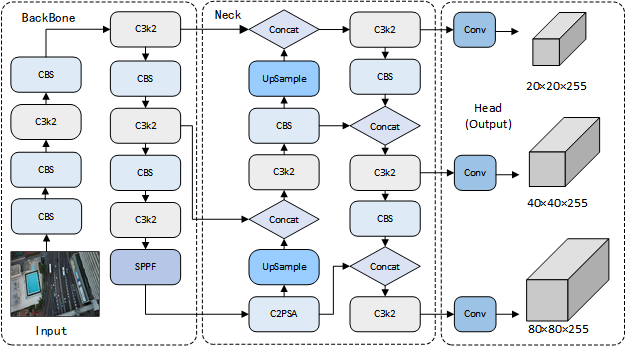
\includegraphics[width=0.8\linewidth]{../figure/yolov11.png}
    }
    \captionsetup{font=footnotesize}
    \bicaption{YOLOv11网络结构}{YOLOv11 network structure diagram.}
    \label{fig:YOLOv11}
\end{figure}

\subsubsection{主干网络}

YOLOv11 的主干网络是其整体架构的核心组成部分,其设计目标是通过改进特征提取能力来提升目标检测的精度,同时在计算效率和模型复杂度之间取得平衡。YOLOv11 的主干网络在继承了 YOLO 系列一贯的高效性和实时性特点的基础上,进一步优化了特征提取的深度和广度,以适应复杂场景下的目标检测需求。

YOLOv11 的主干网络通过多层次的特征金字塔结构(Feature Pyramid Network, FPN),能够提取不同尺度的特征,从而更好地处理不同大小的目标。这种设计特别适用于交通场景中的小目标检测,因为小目标的特征往往分布在较浅的特征层,而大目标则需要更深的特征层来捕捉。
主干网络采用了模块化的设计思路,通过堆叠多个基础模块(如卷积层、池化层和注意力模块)来构建深度网络。这种模块化设计不仅提高了网络的灵活性,还使得网络能够根据具体任务的需求进行调整。
YOLOv11 的主干网络在设计上注重参数的高效利用,通过减少冗余计算和优化网络结构,使得模型在保持高精度的同时,显著降低了参数量和计算复杂度。

YOLOv11 的主干网络基于改进的 CSPDarknet 架构,该架构通过引入跨阶段部分连接(Cross Stage Partial Connections, CSP)技术,显著提高了特征提取的效率和精度。

主干网络首先通过一个输入层接收图像数据,随后经过一系列初始卷积层(Convolutional Layers)进行特征提取。这些卷积层通常采用 $3\times3$ 或 $1\times1$ 的卷积核,用于提取图像的基本特征,如边缘、纹理和颜色信息。初始卷积层的设计旨在快速缩小特征图的尺寸,同时增加特征图的深度,为后续的特征提取奠定基础。
主干网络特征提取过程如图 \ref{fig:YOLOv11_BackBone_input} 所示。
\begin{figure}[htb]
    \centering
    \subfloat{
        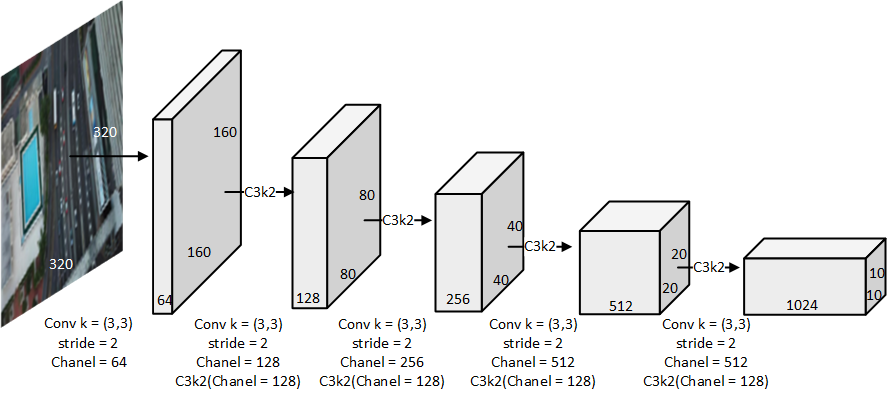
\includegraphics[width=0.8\linewidth]{../figure/yolov11_backbone_input.png}
    }
    \captionsetup{font=footnotesize}
    \bicaption{YOLOv11主干网络输入过程}{YOLOv11 BackBone network structure diagram.}
    \label{fig:YOLOv11_BackBone_input}
\end{figure}

主干网络中包含多个瓶颈模块(Bottleneck Module),这些模块通过 $1\times1$ 卷积层减少特征图的深度,随后通过 $3\times3$ 卷积层进行特征提取,最后再通过 $1\times1$ 卷积层恢复特征图的深度。这种设计在不显著增加计算量的情况下,提高了特征提取的深度和精度。
CBS 模块、BottleNeck 模块如图 \ref{fig:cbs} 、图 \ref{fig:bottleneck} 所示。
\begin{figure}[htb]
    \centering
    \subfloat{
        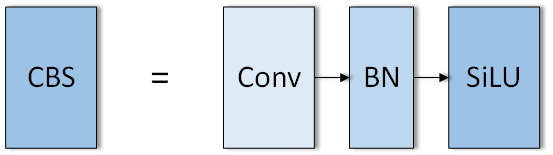
\includegraphics[width=0.5\linewidth]{../figure/cbs.png}
    }
    \captionsetup{font=footnotesize}
    \bicaption{CBS 模块}{YOLOv11 BackBone network structure diagram.}
    \label{fig:cbs}
\end{figure}

\begin{figure}[htb]
    \centering
    \subfloat{
        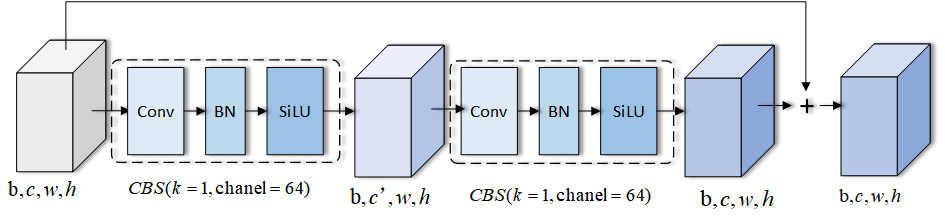
\includegraphics[width=0.9\linewidth]{../figure/bottleneck.png}
    }
    \captionsetup{font=footnotesize}
    \bicaption{BottleNeck模块}{YOLOv11 BackBone network structure diagram.}
    \label{fig:bottleneck}
\end{figure}

CSP 模块是 YOLOv11 主干网络的核心组成部分,其设计灵感来源于残差网络(ResNet)中的残差块。CSP 模块通过将特征图分为两部分,一部分直接传递到下一层,另一部分经过卷积操作后再与前一部分进行拼接,从而减少了计算量并提高了特征提取的效率。CSP 模块的引入不仅增强了网络的特征提取能力,还有效缓解了梯度消失问题,使得网络能够更深层次地学习目标的特征。
C3k2 模块、C2PSA 模块以及 PSA Block 模块如图 \ref{fig:c3k2} 、图 \ref{fig:psablock} 所示。
\begin{figure}[htb]
    \centering
    \subfloat{
        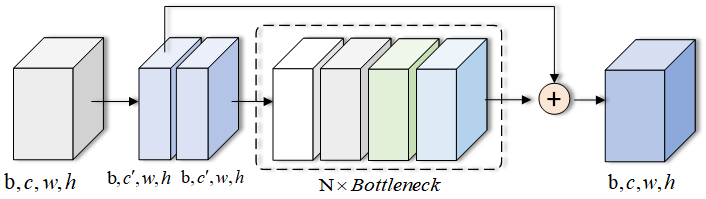
\includegraphics[width=0.8\linewidth]{../figure/c3k2.png}
    }
    \captionsetup{font=footnotesize}
    \bicaption{C3k2 模块}{YOLOv11 BackBone network structure diagram.}
    \label{fig:c3k2}
\end{figure}

\begin{figure}[htb]
    \centering
    \subfloat{
        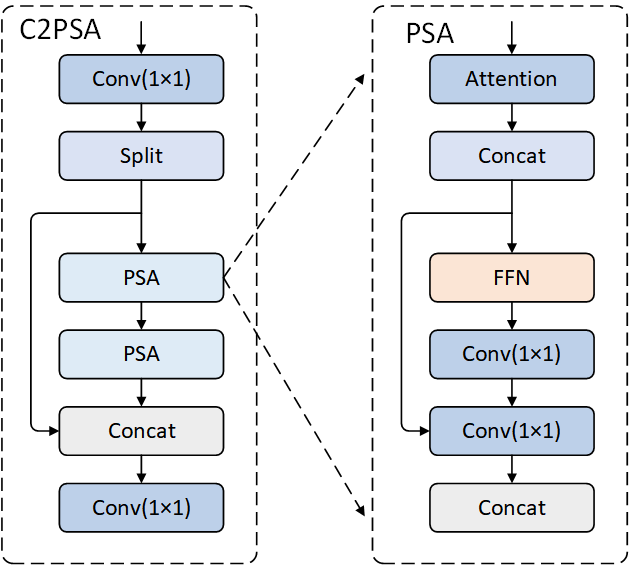
\includegraphics[width=0.6\linewidth]{../figure/pasblock.png}
    }
    \captionsetup{font=footnotesize}
    \bicaption{PSA Block模块}{YOLOv11 BackBone network structure diagram.}
    \label{fig:psablock}
\end{figure}


\subsubsection{特征融合网络}

YOLOv11 的特征融合网络是其整体架构中不可或缺的一部分,其设计目标是通过多尺度特征的融合来提升目标检测的精度和鲁棒性。特征融合网络的设计特点主要体现在以下几个方面:
多尺度特征融合:YOLOv11 的特征融合网络通过整合不同尺度的特征图,使得网络能够同时捕捉到目标的局部细节和全局上下文信息。这种设计特别适用于交通场景中的小目标检测,因为小目标的特征往往分布在较浅的特征层,而大目标则需要更深的特征层来捕捉。
自适应特征加权:YOLOv11 的特征融合网络引入了自适应特征加权机制,通过动态调整不同尺度特征图的权重,使得网络能够更加关注对检测任务更重要的特征。这种机制不仅提高了特征融合的效率,还增强了网络对复杂场景的适应能力。
高效性与实时性:特征融合网络在设计上注重计算效率和实时性,通过优化特征融合的流程和减少冗余计算,使得模型能够在资源受限的设备上高效运行。这对于交通监控系统等实时性要求较高的应用场景具有重要意义。

YOLOv11 的主干网络通过特征金字塔网络(FPN)实现了多尺度特征的融合。FPN 通过自底向上和自顶向下的路径,将不同层次的特征图进行融合,从而生成具有不同尺度的特征金字塔。这种设计使得网络能够同时捕捉到目标的局部细节和全局上下文信息,特别适用于交通场景中大小不一的目标检测。
SPPF 模块如图 \ref{fig:sppf} 所示。
\begin{figure}[htb]
    \centering
    \subfloat{
        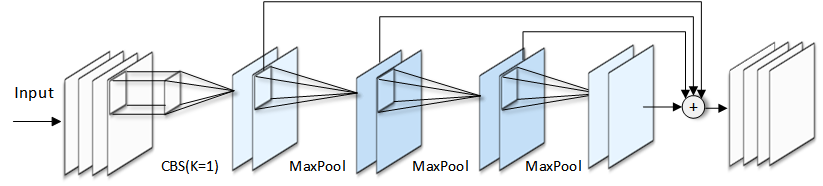
\includegraphics[width=0.85\linewidth]{../figure/sppf.png}
    }
    \captionsetup{font=footnotesize}
    \bicaption{SPPF模块}{YOLOv11 BackBone network structure diagram.}
    \label{fig:sppf}
\end{figure}

PANet 是 YOLOv11 特征融合网络的另一个重要组成部分,其通过在 FPN 的基础上引入横向连接和自底向上的增强路径,进一步优化了特征的融合过程。PANet 的设计使得特征能够在不同尺度之间更高效地流动,从而提高了特征融合的效率和检测的精度。
横向连接:PANet 在 FPN 的基础上增加了横向连接,使得不同尺度的特征图能够直接进行融合,避免了信息的丢失。
自底向上增强路径:PANet 通过自底向上的增强路径,将浅层特征的细节信息传递到深层特征中,从而进一步增强了特征的表达能力。
PANet 网络模型结构如图 \ref{fig:panet} 所示。
\begin{figure}[htb]
    \centering
    \subfloat{
    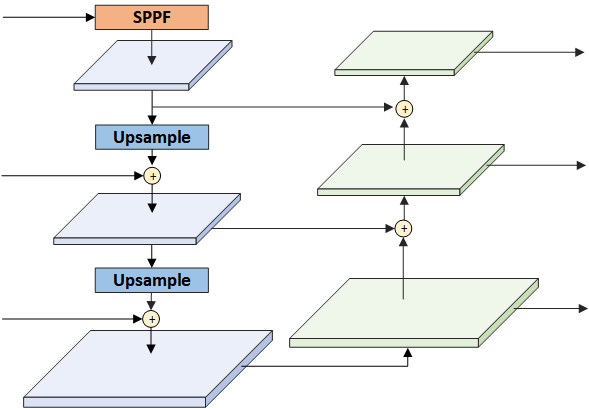
\includegraphics[width=0.6\textwidth]{../figure/panet.png}
    }
    \captionsetup{font=footnotesize}
    \bicaption{PANet网络}{YOLOv11 BackBone network structure diagram.}
    \label{fig:panet}
\end{figure}

YOLOv11 的特征融合网络通过特征融合模块将不同尺度的特征图进行融合,生成具有更高表达能力的特征图。特征融合模块通常采用逐元素加法或拼接操作,结合不同尺度的特征信息,从而提高检测的精度。

\subsection{优化的YOLO网络}

作为一个轻量级目标探测器,YOLOv11以其高效的性能和简单的架构而闻名。 然而,在处理小目标时,YOLOv11存在以下主要问题:(a)特征表征能力不足:YOLOv11采用的特征提取网络没有充分考虑小目标的特征表征,导致小目标的定位精度和检测精度降低。(b)规模感知不足:原始的YOLOv11模型缺乏多尺度目标检测的有效策略,对小目标规模变化的适应性差,容易导致遗漏或误认检查。 这些问题限制了YOLOv11在小目标检测场景中的应用效果。 

为了解决这些问题,本文提出了一系列基于现有方法的改进措施,包括多尺度融合模块SPPC模块、轻量级卷积模块DBSS模块和更高效的损失函数NWD损失函数,以提高检测性能,同时保持模型的轻量级。
用YOLOv11的SPPF模块替换改进的SPPC模块,以提高模型对小目标的检测性能。
使用DBS模块替换YOLOv11中的CBS,并使用DC3k2替换C3k2模块,这可以大大减少计算量,同时保持小目标的检测性能。
使用DBSS注意模块插入到第3层和第5层中,以提高模型对小目标的检测性能 
新方法的模型是EX-YOLO,如图\ref{fig:ex_yolo_detail}所示。

\begin{figure}[htbp]
    \centering
    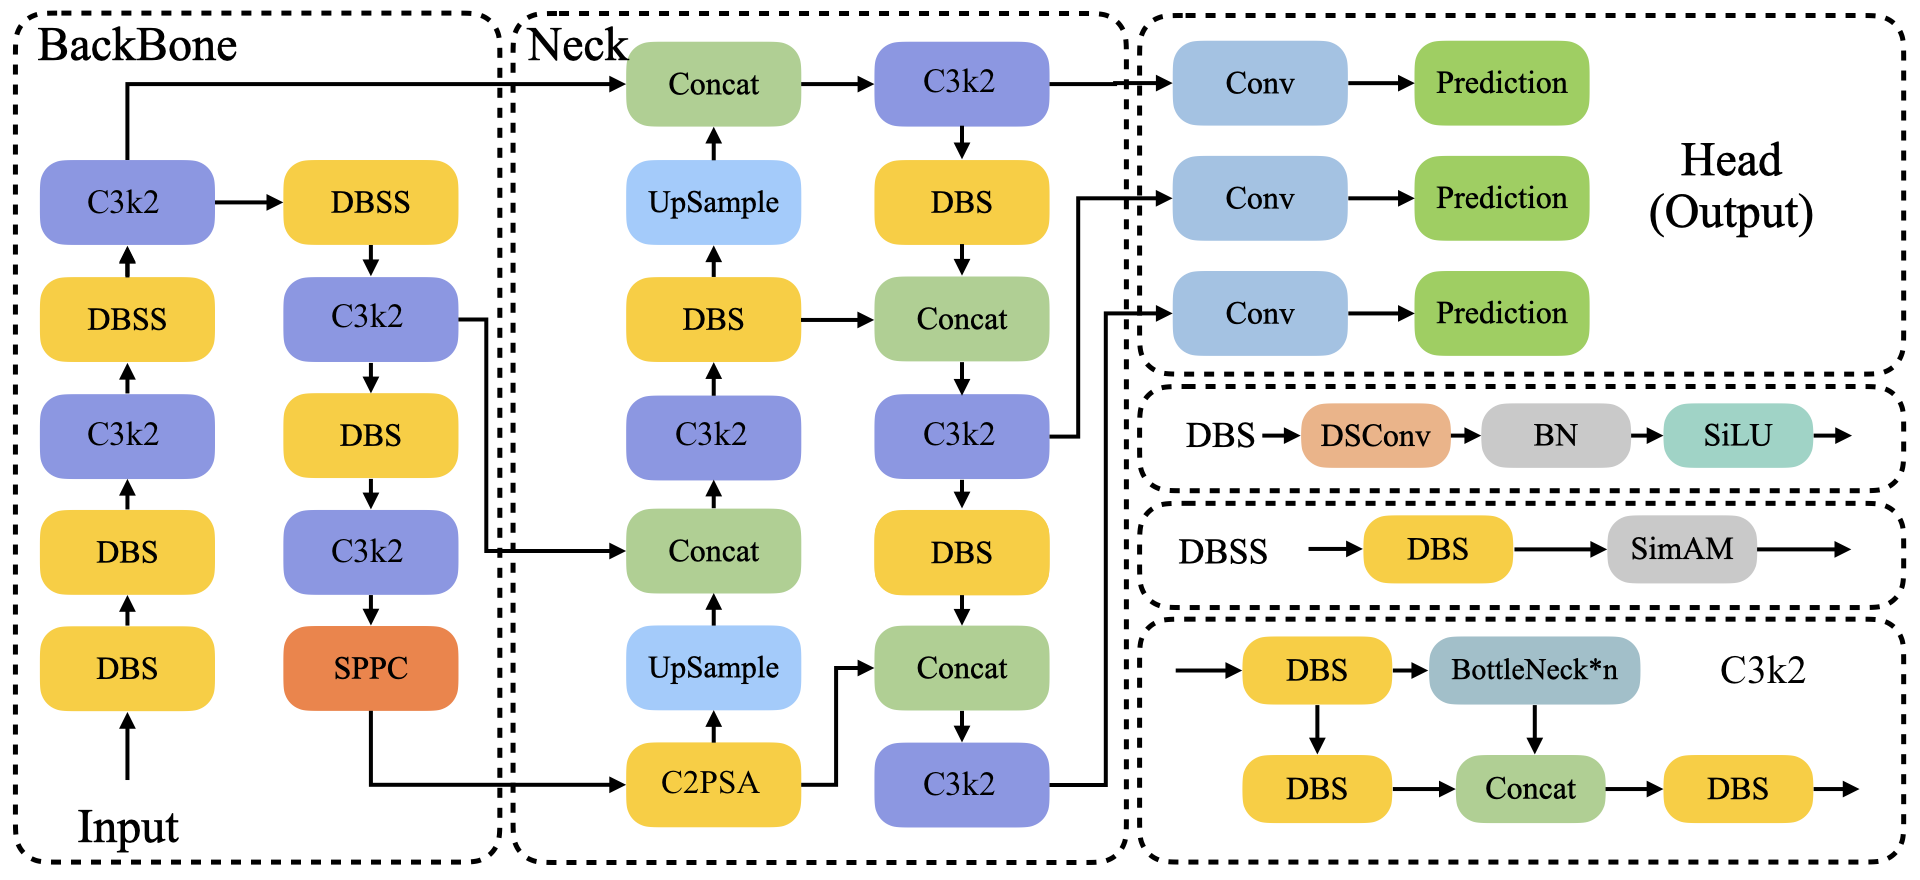
\includegraphics[width=0.9\textwidth]{../figure/ex_yolo_detail.png}
    \captionsetup{font=footnotesize}
    \bicaption{EX-YOLO 网络模型结构}{Some descriptions of the pictures in question.}
    \label{fig:ex_yolo_detail}
\end{figure}


\subsubsection{改进的特征融合模块}

在无人机的小目标检测任务中,传统目标检测算法经常面临特征提取能力不足的问题,特别是在处理中小型目标时,特征图分辨率低,导致关键信息丢失。 
作为一种先进的目标检测算法,尽管YOLOv11在速度和准确性方面表现良好,但在小目标检测任务方面仍有改进的余地。 
为了进一步增强中小型目标模型的特征提取能力,我们提出了SPPC模块。
SPPC模块结合了SPPF模块的多尺度特征提取能力和CAM的特征增强能力,从而提高了中小型目标模型的特征捕获能力,从而提高了mAP。

SPPC模块的结构如图\ref{fig:sppc}所示。
模块的输入特征图首先通过$1\times1$卷积层(cv1)按通道数进行压缩,然后是多个最大池操作(MaxPool),在池过程中将功能增强插入CAM模块中。
最后,所有特征图都通过$1\times1$卷积层(cv2)融合,以输出特征图。

CAM模块的核心设计是通过多尺度卷积运算提取特征,并通过融合增强特征表达。 CAM模块的结构如图\ref{fig:cam}所示,具体公式如下:
\begin{subnumcases}{\label{eq:cam1}}
% \begin{aligned}
    x_1 = Conv(x, kernel=3, dilation=1) \\
    x_2 = Conv(x, kernel=3, dilation=3) \\
    x_3 = Conv(x, kernel=3, dilation=5) 
% \end{aligned}
\end{subnumcases}
公式 \ref{eq:cam1} 中,$x_1$、$x_2$和$x_3$分别表示不同扩展率卷积的输出。
然后,通过$1\times1$卷积进行特征融合:
\begin{subnumcases}{}
    \label{eq:cam2}
% \begin{aligned}
    f_1 = Conv(x_1, kernel=1) \\
    f_2 = Conv(x_2, kernel=1) \\
    f_3 = Conv(x_3, kernel=1)
% \end{aligned}
\end{subnumcases}

最后,CAM模块的输出是:
\begin{equation}
    \label{eq:cam3}
    y = Concat(f_1, f_2, f_3)
\end{equation}

\begin{figure}[htbp]
    \centering
    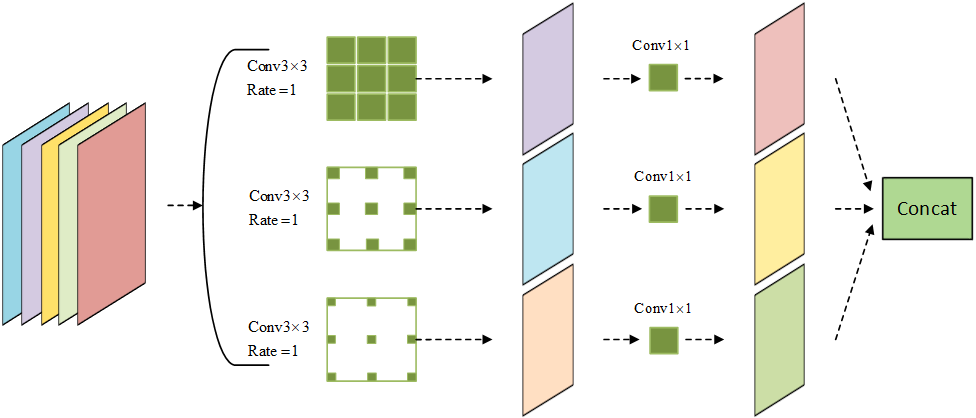
\includegraphics[width=0.7\textwidth]{../figure/CAM.png}
    \captionsetup{font=footnotesize}
    \bicaption{CAM 模块}{Some descriptions of the pictures in question.}
    \label{fig:cam}
\end{figure}

\begin{figure}[htbp]
    \centering
    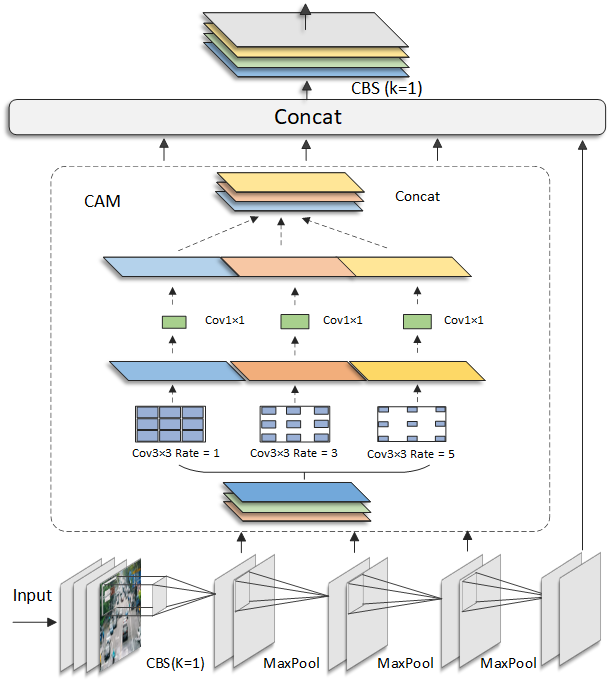
\includegraphics[width=0.6\textwidth]{../figure/SPPC.png}
    \captionsetup{font=footnotesize}
    \bicaption{SPPC 模块}{Some descriptions of the pictures in question.}
    \label{fig:sppc}
\end{figure}

SPPC模块的核心是将CAM模块嵌入到SPPF的池化过程中。 具体实现如下:(a)输入特征图$x$首先通过$1\times1$卷积层(cv1)和输出特征图$y_0$进行压缩。 在$y_0$上执行三个最大池操作(m),每次池后的功能图分别记录为$y_1$、$y_2$、$y_3$:
\begin{subnumcases}{}
% \begin{aligned}
    y_0 = cv_1(x) \\
    y_1 = m(y_0) \\
    y_2 = m(y_1) \\
    y_3 = m(y_2) 
% \end{aligned}
    % y_0 = cv_1(x), y_1 = m(y_0), y_2 = m(y_1), y_3 = m(y_2)
\end{subnumcases}

(b)将CAM模块插入$y_0$、$y_1$、$y_2$,以增强特征表达能力:
\begin{subnumcases}{}
% \begin{aligned}
    y_0' = CAM(y_0) \\
    y_1' = CAM(y_1) \\
    y_2' = CAM(y_2)  
% \end{aligned}
% y_0' = CAM(y_0), y_1' = CAM(y_1), y_2' = CAM(y_2)
\end{subnumcases}

(c)将增强功能图$y_0'$、$y_1'$、$y_2'$与功能图$y_3$进行匹配:
\begin{equation}
    y_{concat} = Concat(y_0', y_1', y_2', y_3)
\end{equation}

(d)最后,通过$1\times1$卷积层(cv2)进行通道融合,并输出最终特征图$y$:
\begin{equation}
    y = cv2(y_{concat})
\end{equation}

SPPC模块可以通过结合SPPF和CAM模块来有效地提取多尺度功能。
SPPF模块通过最大池操作捕获不同尺度的上下文信息,而CAM模块通过多尺度卷积和通道融合进一步增强了特征表达能力。
这种设计使模型能够更好地适应中小型目标的特征提取需求。

\subsubsection{轻量化的卷积模块}

YOLOv11的特征提取网络依靠标准卷积操作(nn.Conv2d)来提取图像的特征信息。 
尽管YOLOv11在目标检测任务中表现出色,但其基于标准卷积层的特征提取网络在计算资源有限的设备上的计算复杂性和资源消耗方面仍存在一些缺点。 
为了降低YOLOv11的计算复杂性和模型参数,并将精度损失最小化,本文介绍了一个轻量级卷积单元——深度可分离卷积(DSC)。 

DSC模块的核心结构如图\ref{fig:DSC}所示。该模块主要由深度卷积、点卷积和动态重量调节模块组成。

(a)深度卷积是每个输入通道上的单独卷积操作。 卷积内核的数量等于输入通道的数量,每个卷积内核只作用于一个通道。 这种方法大大减少了卷积运算的计算量。 深度卷积的数学表达式是:
\begin{equation}
    \label{eq:dsc1}
    O_i = \sum\limits_{k\in{K}}{I_i\otimes{W_{k,i}}}
\end{equation}

公式 \ref{eq:dsc1} 中,$O_i$表示第$i$个输出通道,$I_i$表示第$i$个输入通道,$W_{k,i}$表示作用于$i$通道的卷积内核,$K$表示卷积内核的大小,$\otimes$表示卷积操作。

(b)点卷积是一种$1\times1$卷积操作,用于将深度卷积的输出通道数调整到目标通道数。 点卷积的数学表达式是:
\begin{equation}
    \label{eq:dsc2}
    O = \sum\limits_{i=1}^{C_{in}}I_i\otimes{W_i}
\end{equation}

公式 \ref{eq:dsc2} 中,$O$表示输出通道,$C_{in}$表示输入通道数,$I_i$表示第$i$个输入通道,$W_i$表示点卷积的权重。

(c)为了进一步减少计算量,DSC模块引入了动态权重调整机制。 通过将输入通道划分为多个块,每个块使用共享权重参数$\alpha$来动态调整卷积内核的权重。 具体实现如代码所示。 $\alpha$参数根据块数和通道数展开,并乘以卷积内核权重来生成最终卷积权重。 动态重量调整模块的数学表达式是:
\begin{equation}
    \label{eq:dsc3}
    W_{res} = \alpha\odot{W_{net}}
\end{equation}

公式 \ref{eq:dsc3} 中,$W_{res}$表示调整后的卷积权重,$\alpha$表示动态权重参数,$W_{net}$表示原始卷积权重,$\odot$表示元素乘法。

标准卷积的核心结构如图\ref{fig:nnConv}所示。标准卷积的计算可以通过以下公式来计算:
\begin{equation}
    \label{eq:conv}
    F_{conv} = {C_{in}}\times{C_{out}}\times{K^2}\times{H}\times{W}
\end{equation}

公式 \ref{eq:conv} 中,$C_{in}$表示输入通道数,$C_{out}$表示输出通道数,$K$表示卷积内核的大小,$H$和$W$表示输入特征图的高度和宽度。 

DSC模块的计算体积由两部分组成,深度卷积和点卷积:
\begin{equation}
\begin{aligned}
    F_{depth} &= {C_{in}}\times{K^2}\times{H}\times{W} \\
\end{aligned} 
\label{eq:dsconv_depth}
\end{equation}

\begin{equation}
\begin{aligned}
    F_{point} &= {C_{in}}\times{C_{out}}\times{H}\times{W} \\
\end{aligned} 
\label{eq:dsconv_point}
\end{equation}

\begin{equation}
\begin{aligned}
    F_{DSC} &= F_{depth} + F_{point} \\
            &= {C_{in}}\times\left({K^2+C_{out}}\right)\times{H}\times{W}
\end{aligned} 
\label{eq:dsconv}
\end{equation}

通过比较方程\ref{eq:conv}和方程\ref{eq:dsconv},可以发现DSC模块的计算量显著降低。

\begin{figure}[htbp]
    \centering
    \subfloat {
        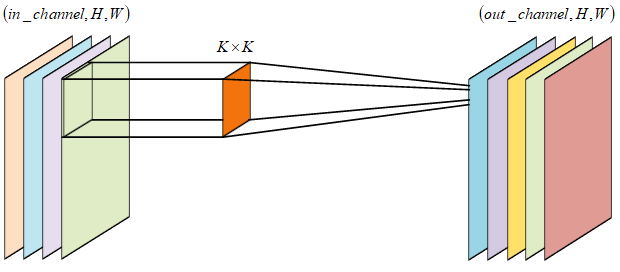
\includegraphics[width=0.7\textwidth]{../figure/nnConv.png}
    }
    \captionsetup{font=footnotesize}
    \bicaption{标准卷积模块}{Some descriptions of the pictures in question.}
    \label{fig:nnConv}
\end{figure}

\begin{figure}[htbp]
    \centering
    \subfloat {
        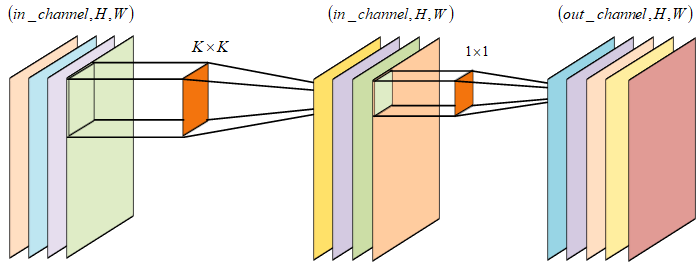
\includegraphics[width=0.7\textwidth]{../figure/DSC.png}
    } 
    % \caption{Compared nn.Conv Module with DSC Module}
    \captionsetup{font=footnotesize}
    \bicaption{DSC卷积模块}{Some descriptions of the pictures in question.}
    \label{fig:DSC}
\end{figure}

SimAM(Simple Attention Module)是一个简单且无参数的注意力模块\cite{simam}。 
SimAM通过推断特征图的3D注意力权重并优化能量函数来找出每个神经元的重要性,从而提高了各种视觉任务的性能。
SimAM通过计算特征图中每个位置的激活值与整体特征之间的相似性来动态调整每个位置的特征权重。
与传统的注意力机制相比,SimAM不依赖额外的卷积层或池操作,计算复杂性低,并且易于集成到现有的网络架构中。

SimAM的实现基于简单的数学运算,设输入特征图$x\in{R^{{B}\times{C}\times{H}\times{W}}}$,其中$B$、$C$、$H$和$W$分别表示批次数、通道数、高度和宽度。其核心公式如下:

(a)计算每个通道特征图的空间维度的平均值:
\begin{equation}
    \label{eq:simam1}
    \mu_c = \frac{1}{{H}\times{W}}\sum\limits_{i=1}^{H}\sum\limits_{j=1}^{W}x_{c,i,j}
\end{equation}

公式 \ref{eq:simam1} 中,$\mu_c$表示$c$通道的平均值。

(b)计算每个位置的激活值与通道平均值之间的相似性:
\begin{equation}
    \label{eq:simam2}
    y_{c,i,j} = \frac{(x_{c,i,j}-\mu_c)^2}{4\left(\sum_{k=1}^{H}\sum_{l=1}^{W}(x_{c,i,j}-\mu_c)^2/n+\lambda \right)}+0.5
\end{equation}

公式 \ref{eq:simam2} 中,$n={H}\times{W}-1$,$\lambda$是一个非常小的正则化常数,用于避免分母为$0$。

(c)使用Sigmoid激活函数将相似性归一化,并将归一化相似性作为输入特征图的权重应用。
\begin{equation}
    \label{eq:simam3}
    output_{c,i,j} = x_{c,i,j} \cdot \sigma(y_{c,i,j})
\end{equation}

DBSS模块连接DSC卷积单元和SimAM注意模块,以实现轻量级卷积计算和集成SimAM注意模块的轻量级模块。

\begin{figure}[htbp]
    \centering
    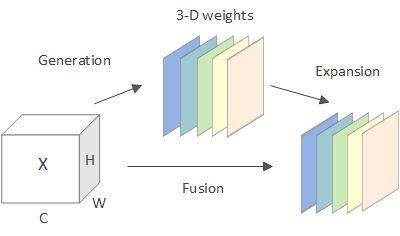
\includegraphics[width=0.6\textwidth]{../figure/SimAM.png}
    \captionsetup{font=footnotesize}
    \bicaption{SamAM 模块}{Some descriptions of the pictures in question.}
    \label{fig:SimAM}
\end{figure}

\subsubsection{更高效的损失函数}

在无人机的目标检测任务中,目标通常具有体积小、特征不显眼、背景复杂等特点,这对目标检测算法提出了更高的要求。 在处理小目标时,传统的IoU损失函数有一定的局限性。
IoU损失函数只考虑预测框和真实框之间的重叠区域。 对于小目标,预测框和真实框之间的小偏差可能会导致大的定位误差,而IoU损失函数对这些偏差不太敏感。

为了进一步提高小目标的检测性能,我们引入了NWD框损耗函数,并将其与DIoU箱损耗功能相结合。
NWD损失函数可以通过计算预测框和真实框之间的空间和规模差异来更准确地评估预测框和真实框之间的相似性,从而提高模型捕捉小目标的能力。

DIoU损失函数基于IoU损失函数的改进版本,其核心的想法是通过引入预测框和真实框中心点之间的距离来提高损失函数对空间位置的敏感性。
具体定义如下:
\begin{equation}
    \label{eq:diou}
    L_{DIoU} = 1 - \frac{A\cap{B}}{A\cup{B}} + \frac{\rho^2(c_p, c_g)}{c^2}
\end{equation}
公式 \ref{eq:diou} 中,$A\cap{B}$表示预测框和真实框的交集面积,$A\cup{B}$表示预测框和真实框的并集面积,$\rho^2(c_p, c_g)$表示预测框的中心点$c_p$和真实框的中心点$c_g$之间的欧几里得举例,$c$表示可以覆盖预测框和真实框最小闭合的对角线长度。

NWD框损失函数是通过计算预测框和真实框之间的空间和规模差异来评估的。 两者之间的相似性。
具体定义如下:
给定预测框$\mathbf{p}$和地面真理边界框$\mathbf{g}$,其中心坐标是$\mathbf{c}_p = (x_p, y_p)$和$\mathbf{c}_g = (x_g, y_g)$,宽度和高度分别为$(w_p, h_p)$和$(w_g, h_g)$。 NWD损失函数的定义是:
\begin{equation}
    L_{NWD} = \exp\left(-\frac{\sqrt{D_W}}{c}\right)
    \label{eq:nwd}
\end{equation}

公式 \eqref{eq:nwd} 中,Wasserstein距离$D_W$是:
\begin{equation}
    D_W = (\Delta x)^2 + (\Delta y)^2 + \frac{(w_p - w_g)^2 + (h_p - h_g)^2}{4} + \epsilon
    \label{eq:dw}
\end{equation}

公式 \eqref{eq:dw} 中,$\Delta x = x_p - x_g$,$\Delta y = y_p - y_g$,$\epsilon$是一个非常小的常数,以避免除法错误,$c$是用于调整距离变焦的常数。以DIoU损失函数和NWD盒子损失函数之和作为YOLOv11的盒子损失函数:
\begin{equation}
    L_{box\_loss} = \frac{L_{DIoU}+L_{NWD}}{2}
\end{equation}

通过将DIoU损失函数和NWD损失函数相加来取平均值,我们可以进一步提高模型对小目标的检测能力,同时保持大多数目标的DIoU损失函数的检测性能。
这种组合可以充分利用两种损失函数的优势,从而提高模型的整体检测性能。


\subsection{交通目标检测实验结果和分析}

新算法在TT100K数据集\cite{tt100k}和VisDrone数据集\cite{vd}上进行训练和测试,以改进每个阶段,并与YOLOv11s\cite{yolov11}进行比较。
为了在不降低其他比例目标的精度的情况下通过算法验证不同尺寸目标的检测精度,对TT100K和VisDrone的数据集进行了比较实验。
最后,在不同场景中选择复杂的场景图片,并将拟议算法的检测效果与实际场景中的YOLOv11s、YOLOv10s\cite{yolov10}和YOLOv9s\cite{yolov9}算法进行比较。

\subsubsection{数据集}

在目标检测领域,特别是对无人机小目标检测任务的研究,选择适当的数据集对于验证算法的性能至关重要。
这个实验采用了两个数据集,TT100K和VisDrone。
为了评估改进的YOLOv11算法,小目标检查测量任务的性能提供了强大的支持。

TT00K数据集由中国清华大学和腾讯团队收集。
数据集由无人机获得,是交通标志的目标识别数据集;它是在不同的场景、天气和光线下收集的,因此在复杂的环境中有许多小目标。
数据集还提供了一些属性,如场景可见性、对象类和遮挡。
图\ref{fig:tt100k_figure}显示了TT100K数据集中的一些数据。
从图\ref{fig:tt100k_figure}中可以看出,TT100K数据集中的小目标数量很小,分布不均匀,分布不在中心,并且有许多目标类别。

\begin{figure}[htbp]
    \centering
    \subfloat {
    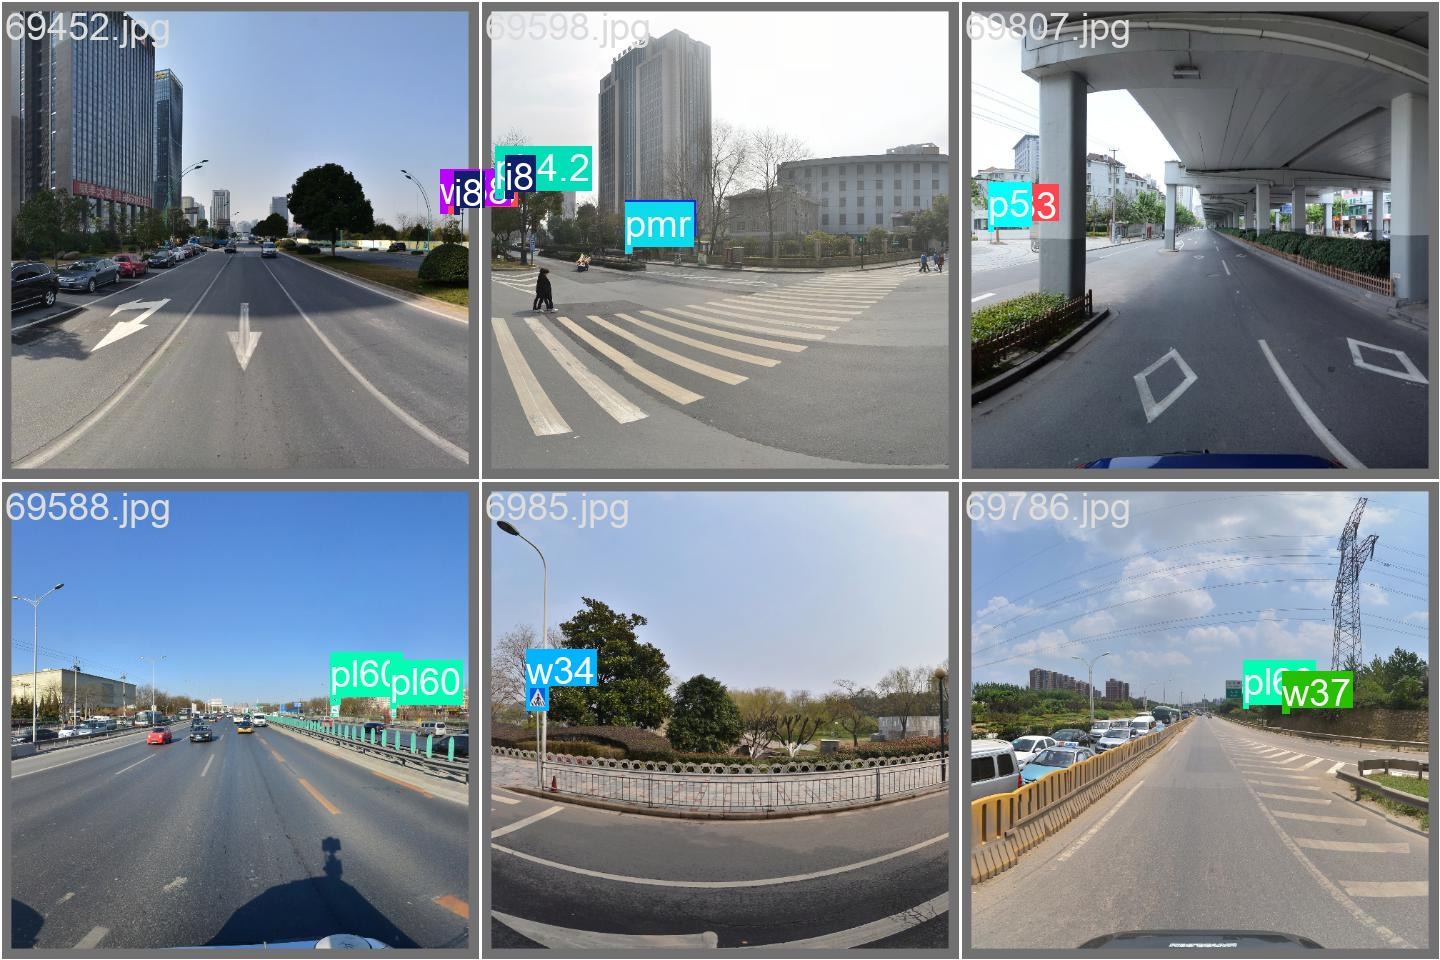
\includegraphics[width=0.8\textwidth]{../figure/TT100K.png}
    }
    \captionsetup{font=footnotesize}
    \bicaption{TT100K 数据集}{Some descriptions of the pictures in question.}
    \label{fig:tt100k_figure}
\end{figure}

VisDrone数据集是天津大学机器学习和数据挖掘实验室AISKYEYE团队创建的大规模基准数据集,专为无人机图像和视频分析中的各种计算机视觉任务而设计。
它包含288个视频剪辑、261,908帧图像和10,209个静态图像,涵盖了不同城市、环境、物体和密度的场景,并在各种天气和照明条件下收集。
图\ref{fig:vd_figure}显示了VisDrone数据集中的一些数据。
从图\ref{fig:vd_figure}中可以观察到,VisDrone数据集有大量的小目标和很少的目标类别。

\begin{figure}[htbp]
    \centering
    \subfloat {
    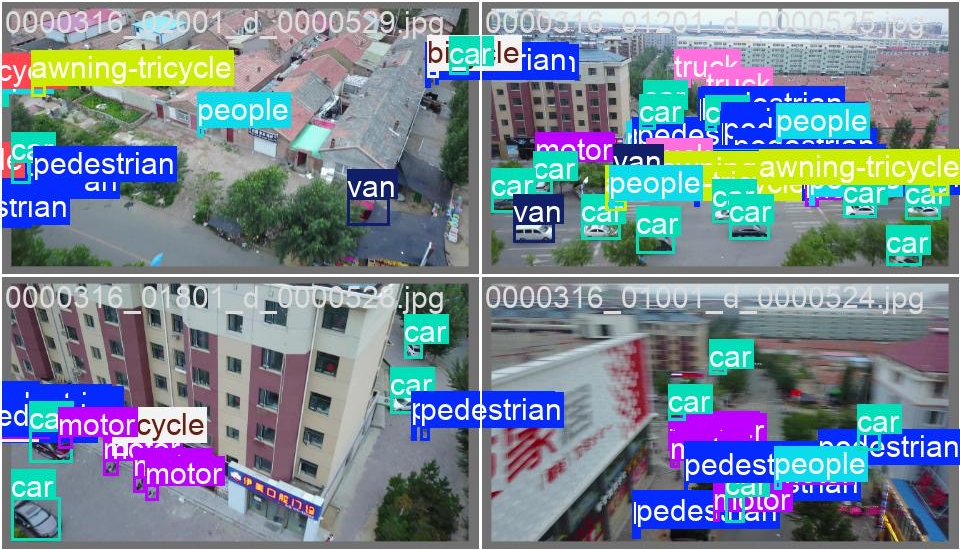
\includegraphics[width=0.8\textwidth]{../figure/VisDrone.png}
    }
    \captionsetup{font=footnotesize}
    \bicaption{VisDrone 数据集}{Some descriptions of the pictures in question.}
    \label{fig:vd_figure}
\end{figure}

虽然TT100K和VisDrone数据集不是直接基于无人机视角,但它们包含的目标类型与无人机在实际应用中需要识别的目标高度一致。
交通标志是交通检查、智能交通和其他领域中无人机的重要识别对象,而人、自行车、摩托车和汽车是安全监控、城市交通管理和其他场景中无人机的关键检测目标。
通过对这些数据集进行实验,可以间接评估改进的YOLOv11算法在无人驾驶飞行器小型目标检测任务中的潜力和优势。
与此同时,这些数据集的复杂场景和多样化的样本也为算法的泛化能力和鲁棒性测试提供了良好的基础,这有利于在不同情况下发现算法的优缺点,并为进一步优化算法以满足无人机的实际应用需求提供了重要的参考。

\subsubsection{实验环境}

本文中用于实验的系统、系统硬件设施和软件平台如表\ref{tab:environment}所示。
\begin{table}[htbp]
    \centering
    \captionsetup{font=footnotesize}
    \bicaption{实验环境设置}{Symbol cross-reference table}
    \label{tab:environment}
    \begin{tabular}{cc}
        \toprule
        List              & Version            \\ 
        \midrule
        Operating System  & Ubuntu 22          \\
        Memory            & 64G RAM            \\
        CPU               & Intel i9-13900K    \\
        GPU               & NVIDIA GTX4090 GPU \\
        Cuda              & cu121              \\
        Python            & 3.11               \\
        \bottomrule
    \end{tabular}
\end{table}

\subsubsection{实验结果和分析}

在这项研究中,我们通过比较实验评估了EX-YOLO模型(our)在2个不同数据集中,包括TT100K和VisDrone数据集上的性能,以验证小目标检测和多尺度目标检测的改进方法的有效性。
通过将其与基准模型YOLOv11s、YOLOv10s和YOLOv9s进行比较,评估改进模型在各种指标上的性能。

\begin{table}[htbp]
    \centering
    \captionsetup{font=footnotesize}
    \bicaption{在TT100K数据集上的对比实验结果}{Symbol cross-reference table}
    \label{tab:compare_studies_tt100k}
    \begin{tabular}{p{0.13\textwidth}p{0.13\textwidth}p{0.19\textwidth}p{0.1\textwidth}p{0.07\textwidth}p{0.07\textwidth}p{0.07\textwidth}}
        \toprule
        模型       & 参数量 MB & 计算量 GFLOPs & $mAP_{0.5}$   & P     & R     & FPS \\ 
        \midrule
        YOLOv11s     & 9.5           & 21.8          & 0.877          & 0.878  & 0.777 & 94.3 \\
        YOLOv10s     & 8.2           & 25.4          & 0.850          & 0.776  & 0.752 & 88.5 \\
        YOLOv9s      & 7.5           & 27.2          & \textbf{0.906} & 0.914  & 0.818 & 90.9 \\
        \textbf{our} & 11.4          & \textbf{17.0} & 0.893          & 0.875  & 0.830 & 84.7 \\
        \bottomrule
    \end{tabular}
\end{table}

\begin{figure}[htbp]
    \centering
        \subfloat[EX-YOLO\label{fig:tt100k_ex_cmn}]{
            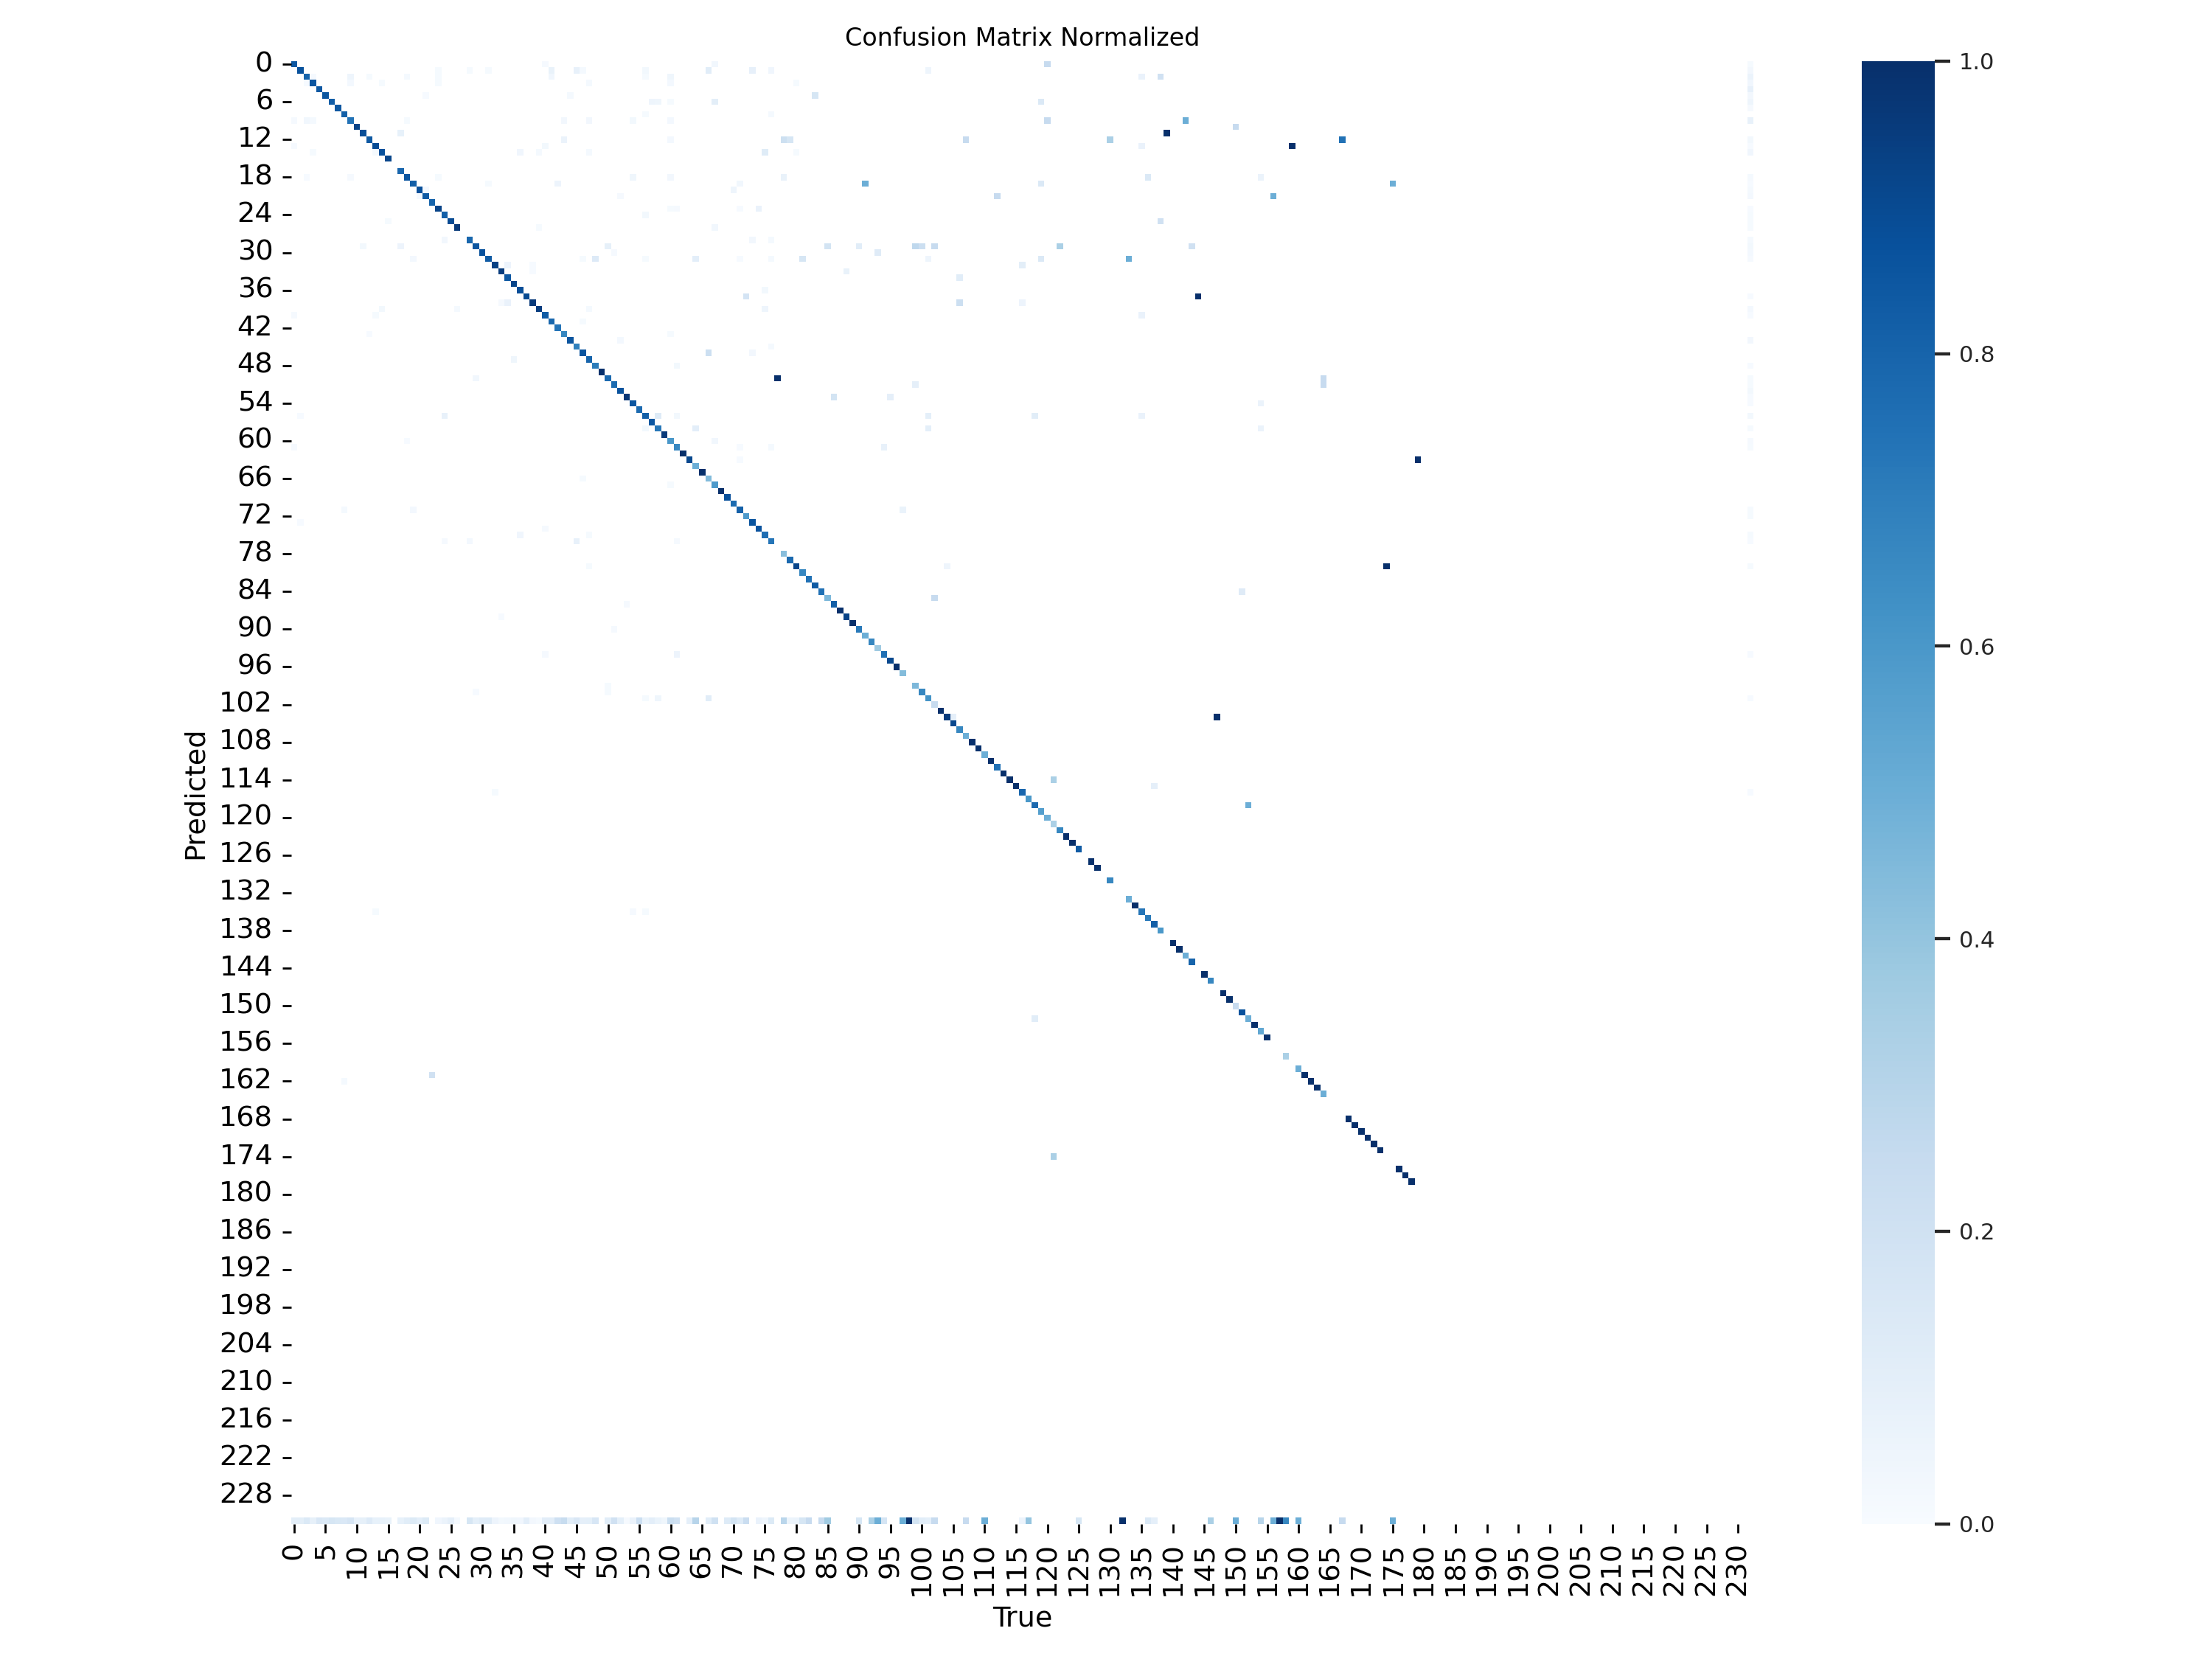
\includegraphics[width=0.4\textwidth]{../figure/tt100k_ex_confusion_matrix_normalized.png}
        }
        \subfloat[YOLOv11s\label{fig:tt100k_11s_cmn}]{
            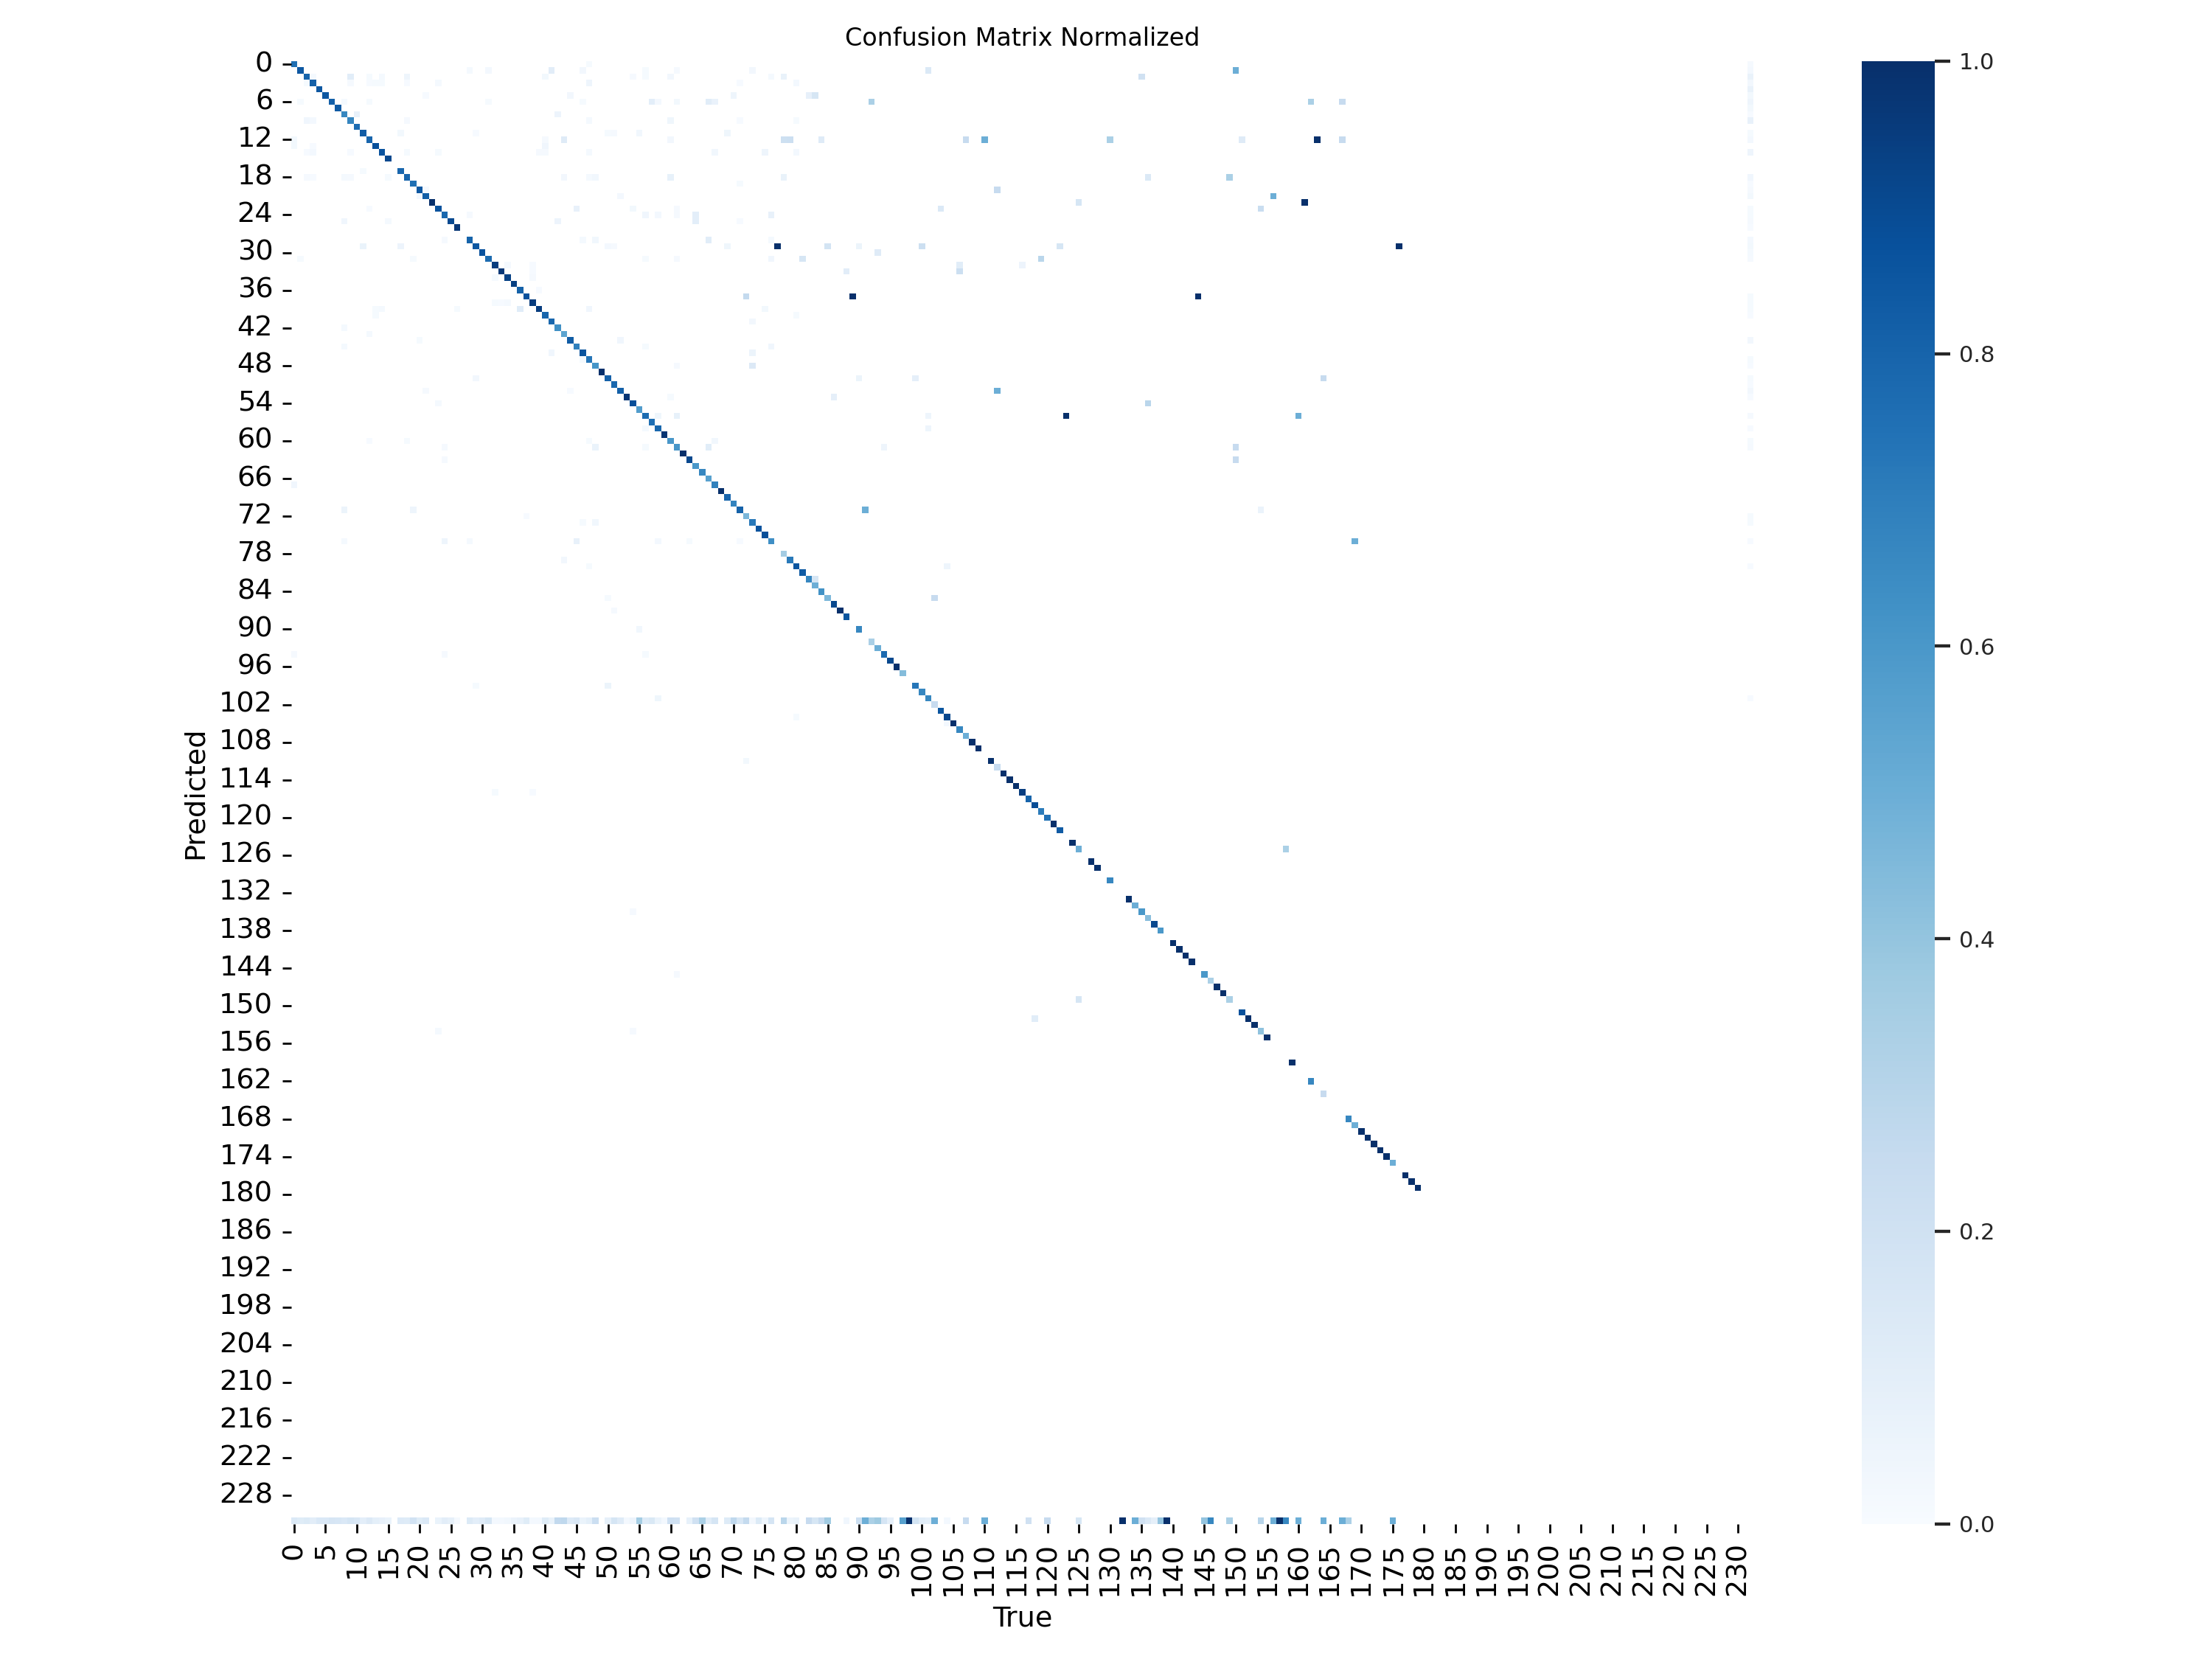
\includegraphics[width=0.4\textwidth]{../figure/tt100k_v11s_confusion_matrix_normalized.png}
        } \\
        \subfloat[YOLOv10s\label{fig:tt100k_10s_cmn}]{
            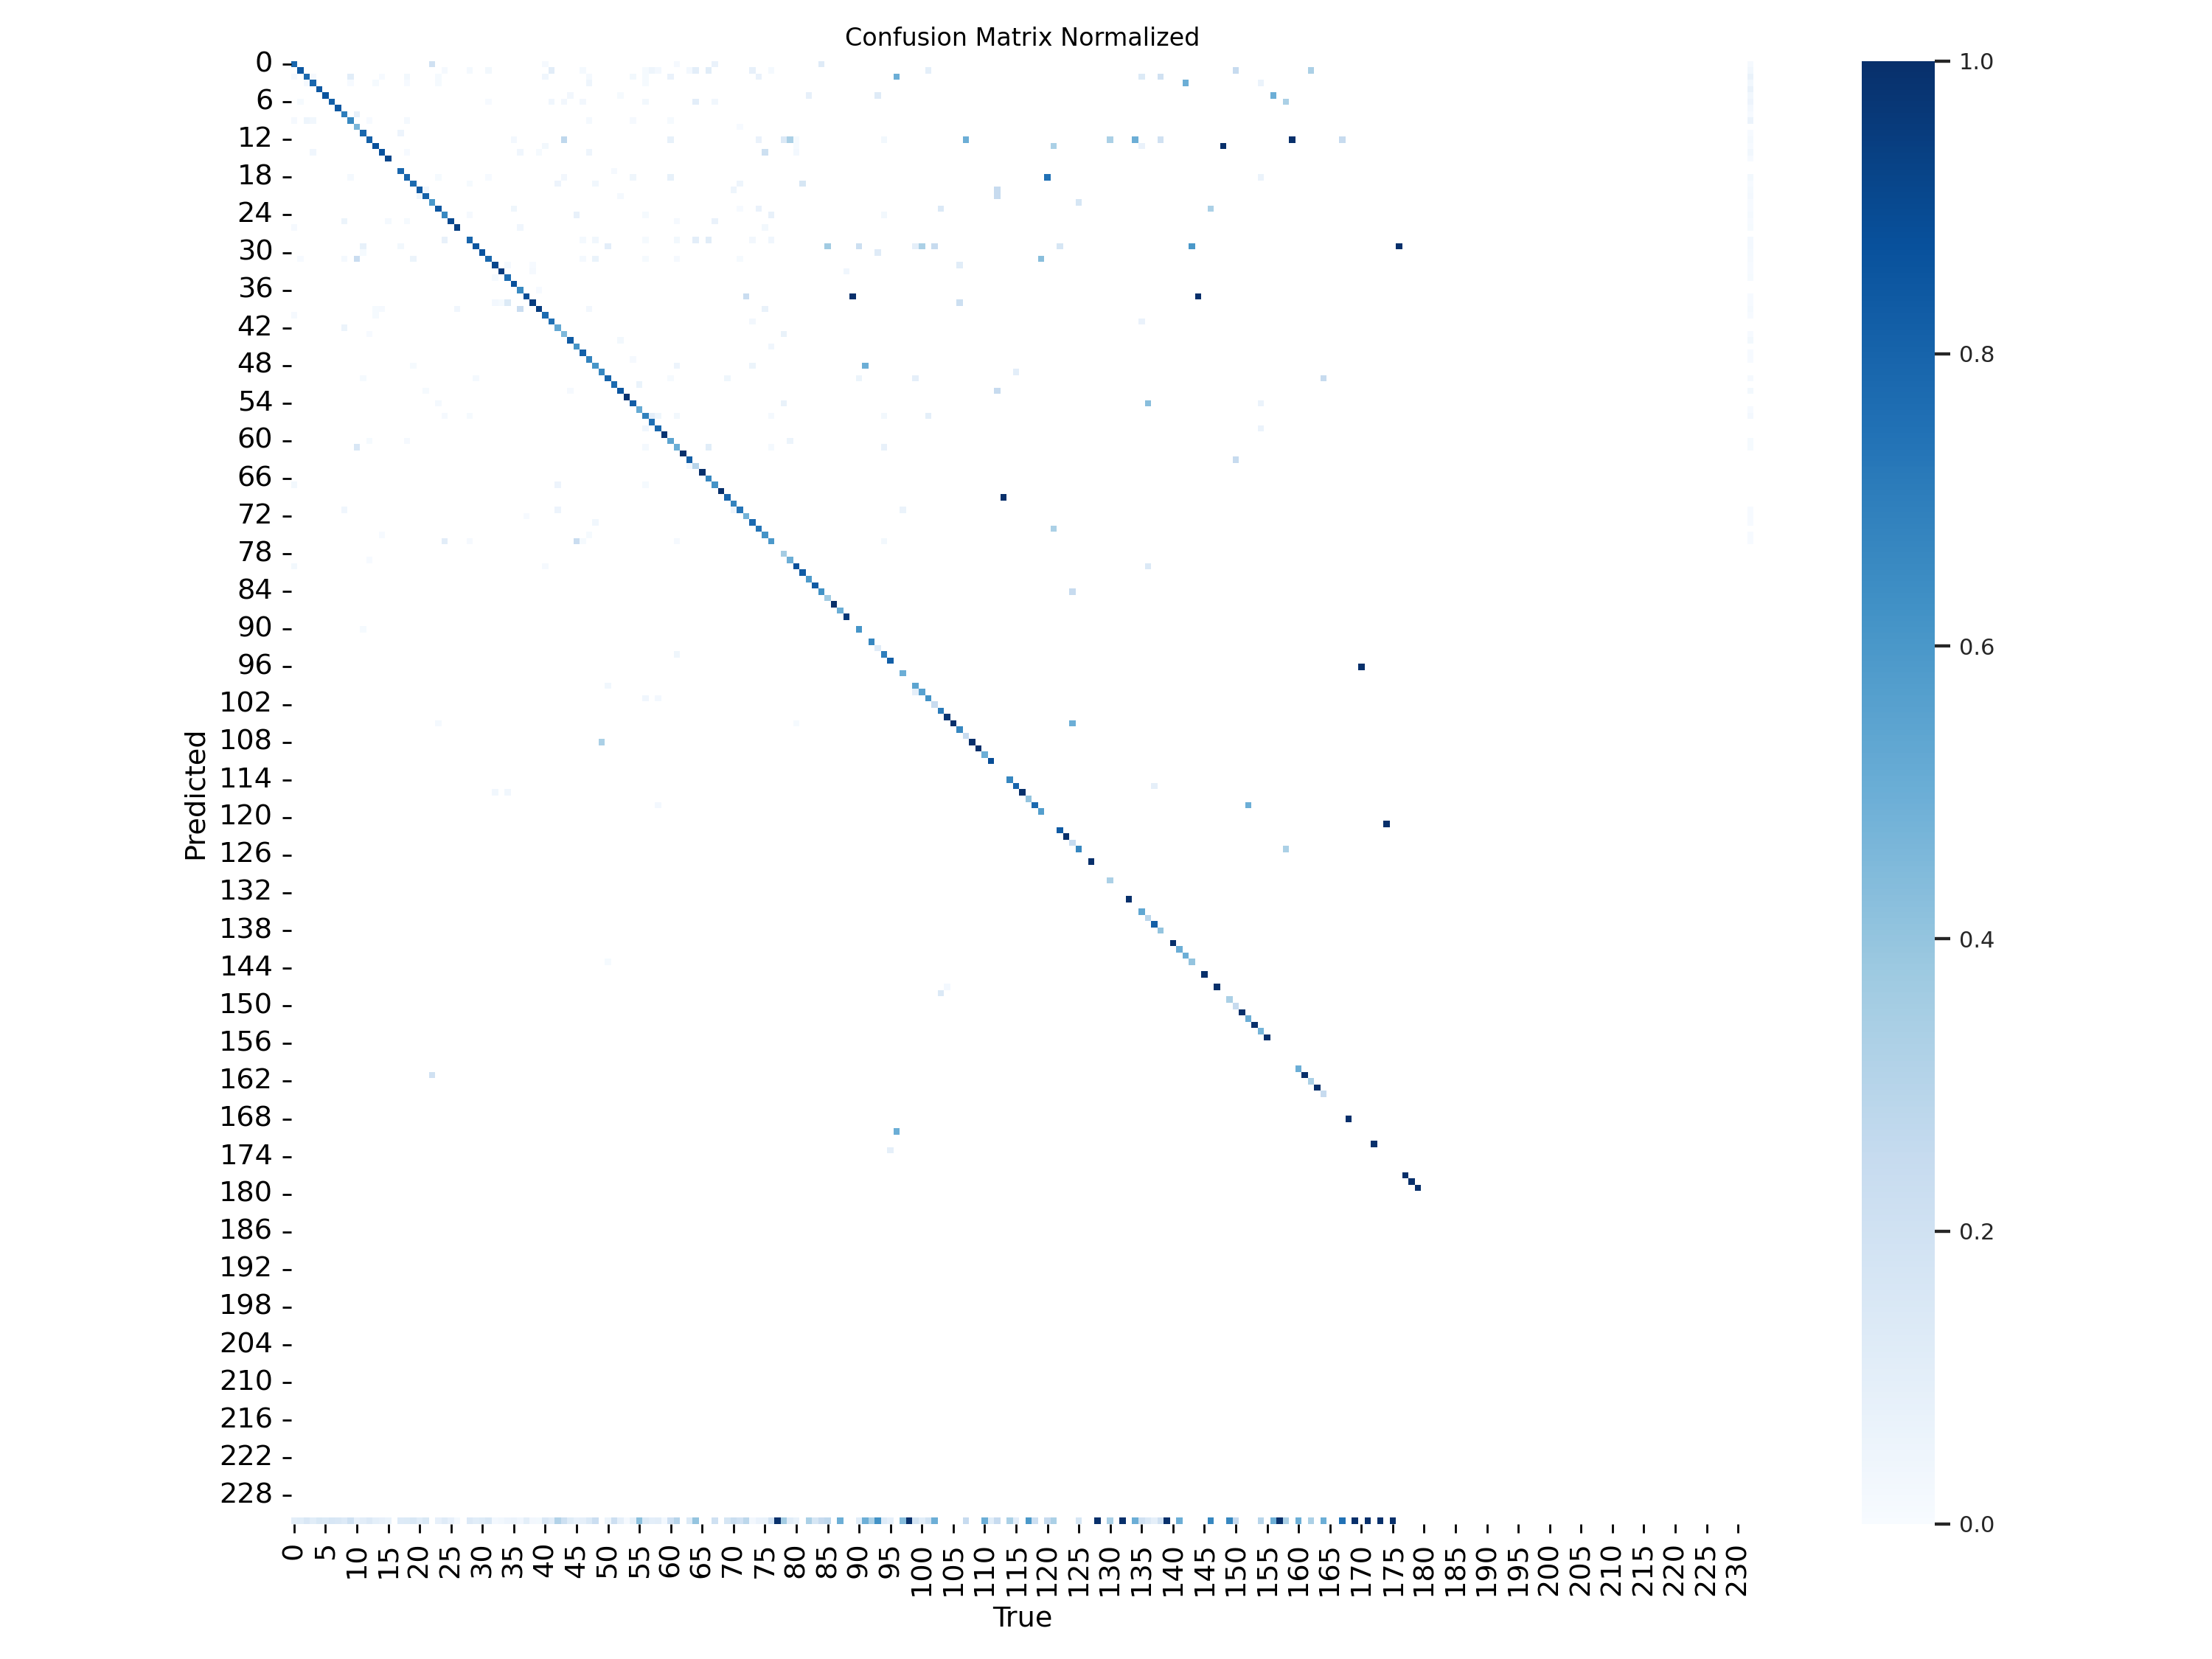
\includegraphics[width=0.4\textwidth]{../figure/tt100k_v10s_confusion_matrix_normalized.png}
        }
        \subfloat[YOLOv9s\label{fig:tt100k_9s_cmn}]{
            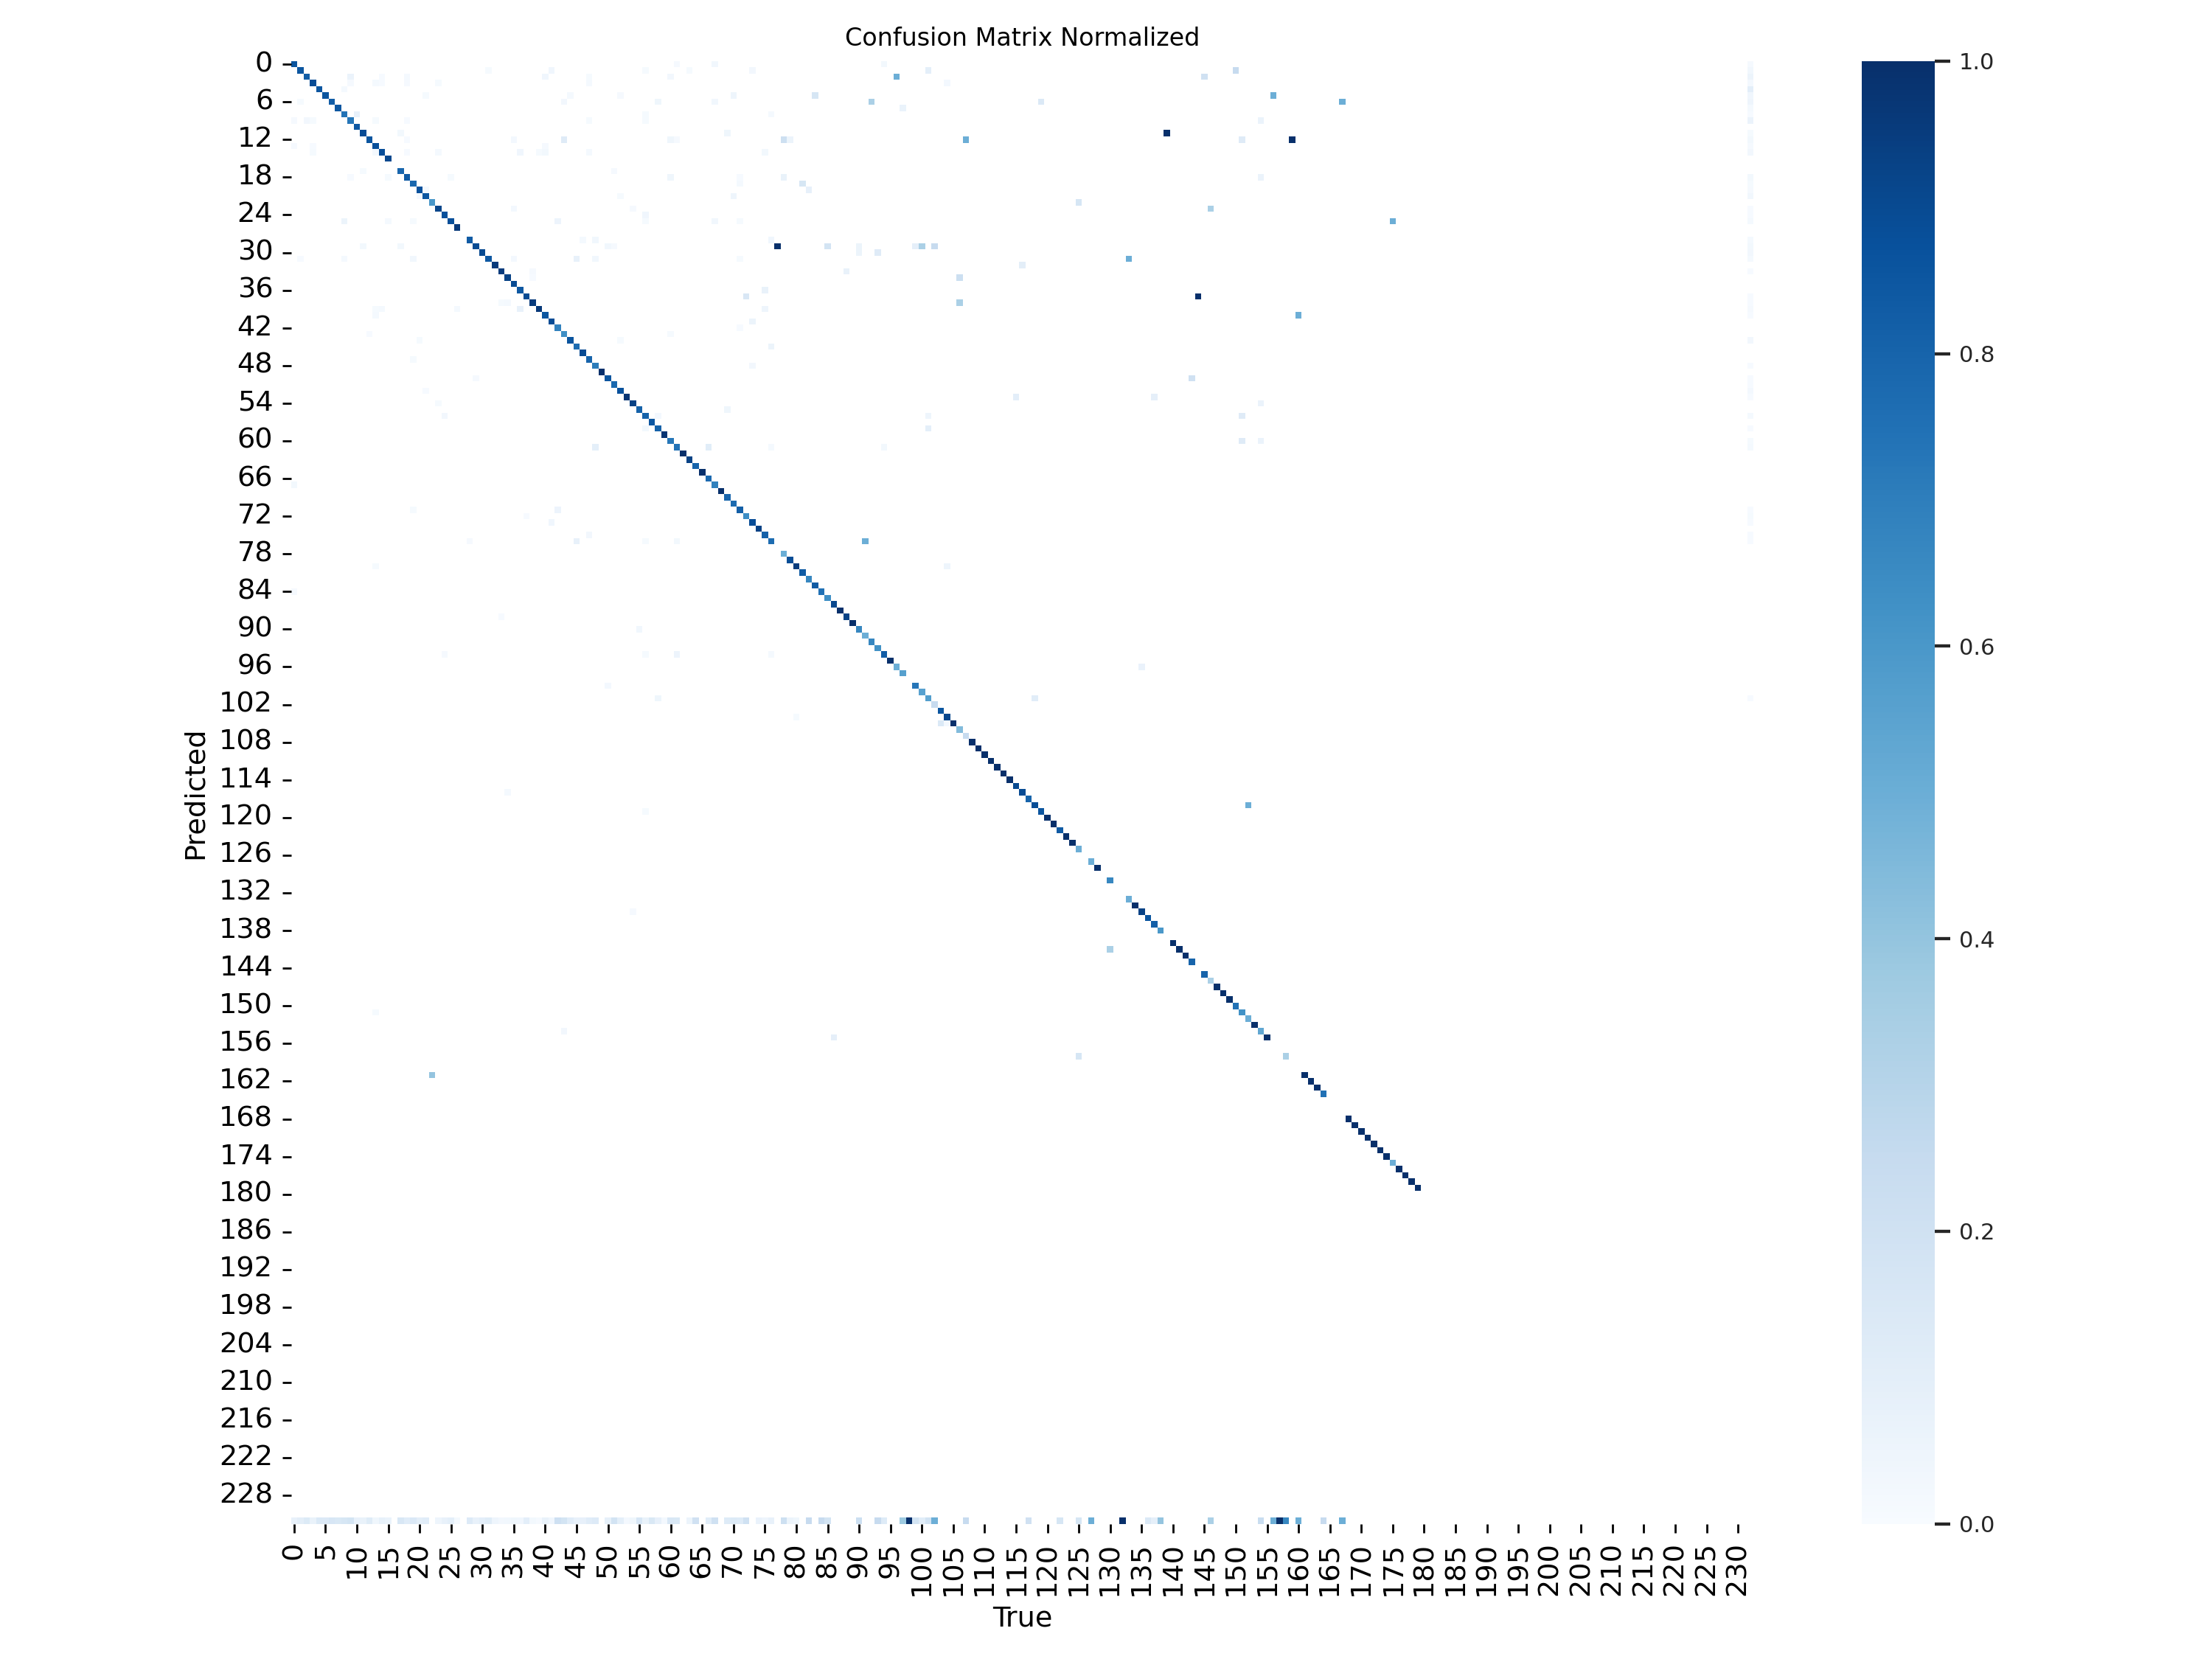
\includegraphics[width=0.4\textwidth]{../figure/tt100k_v9s_confusion_matrix_normalized.png}
        }
    \captionsetup{font=footnotesize}
    \bicaption{不同的网络模型在TT100K数据集上的归一化混淆矩阵}{Symbol cross-reference table}
    \label{fig:tt100k_cmn}
\end{figure}

\begin{figure}[htbp]
    \centering
        \subfloat[EX-YOLO\label{fig:tt100k_ex_f1}]{
            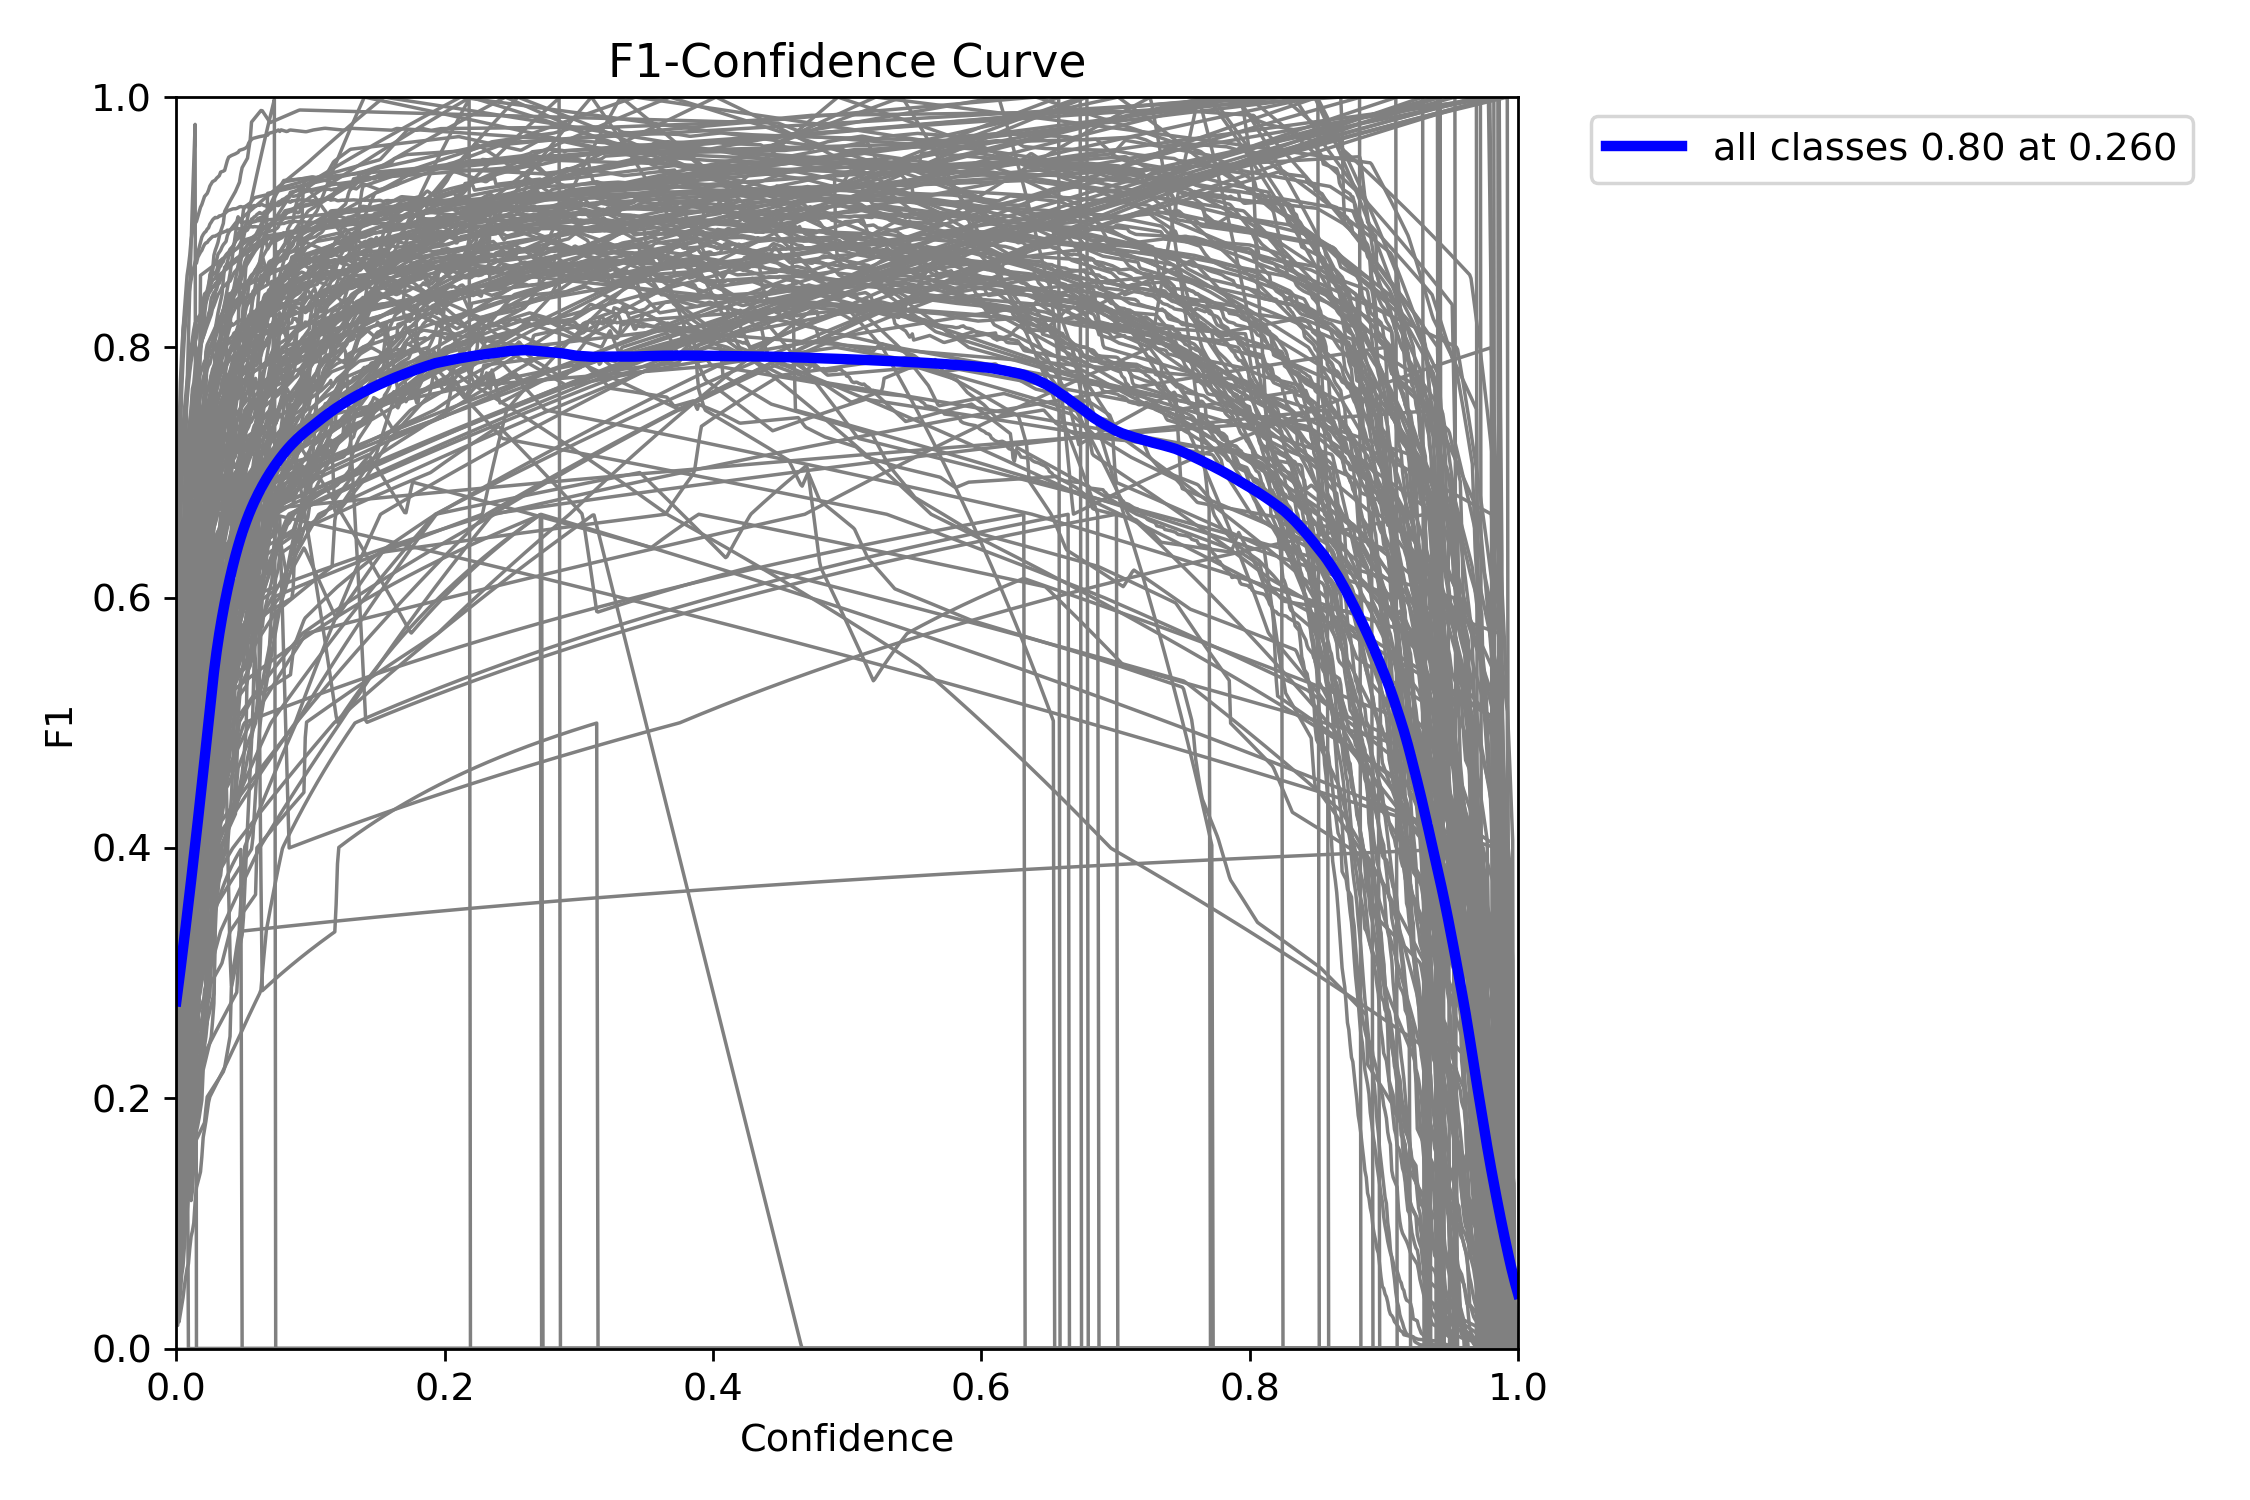
\includegraphics[width=0.4\textwidth]{../figure/tt100k_ex_F1_curve.png}
        }
        \subfloat[YOLOv11s\label{fig:tt100k_11s_f1}]{
            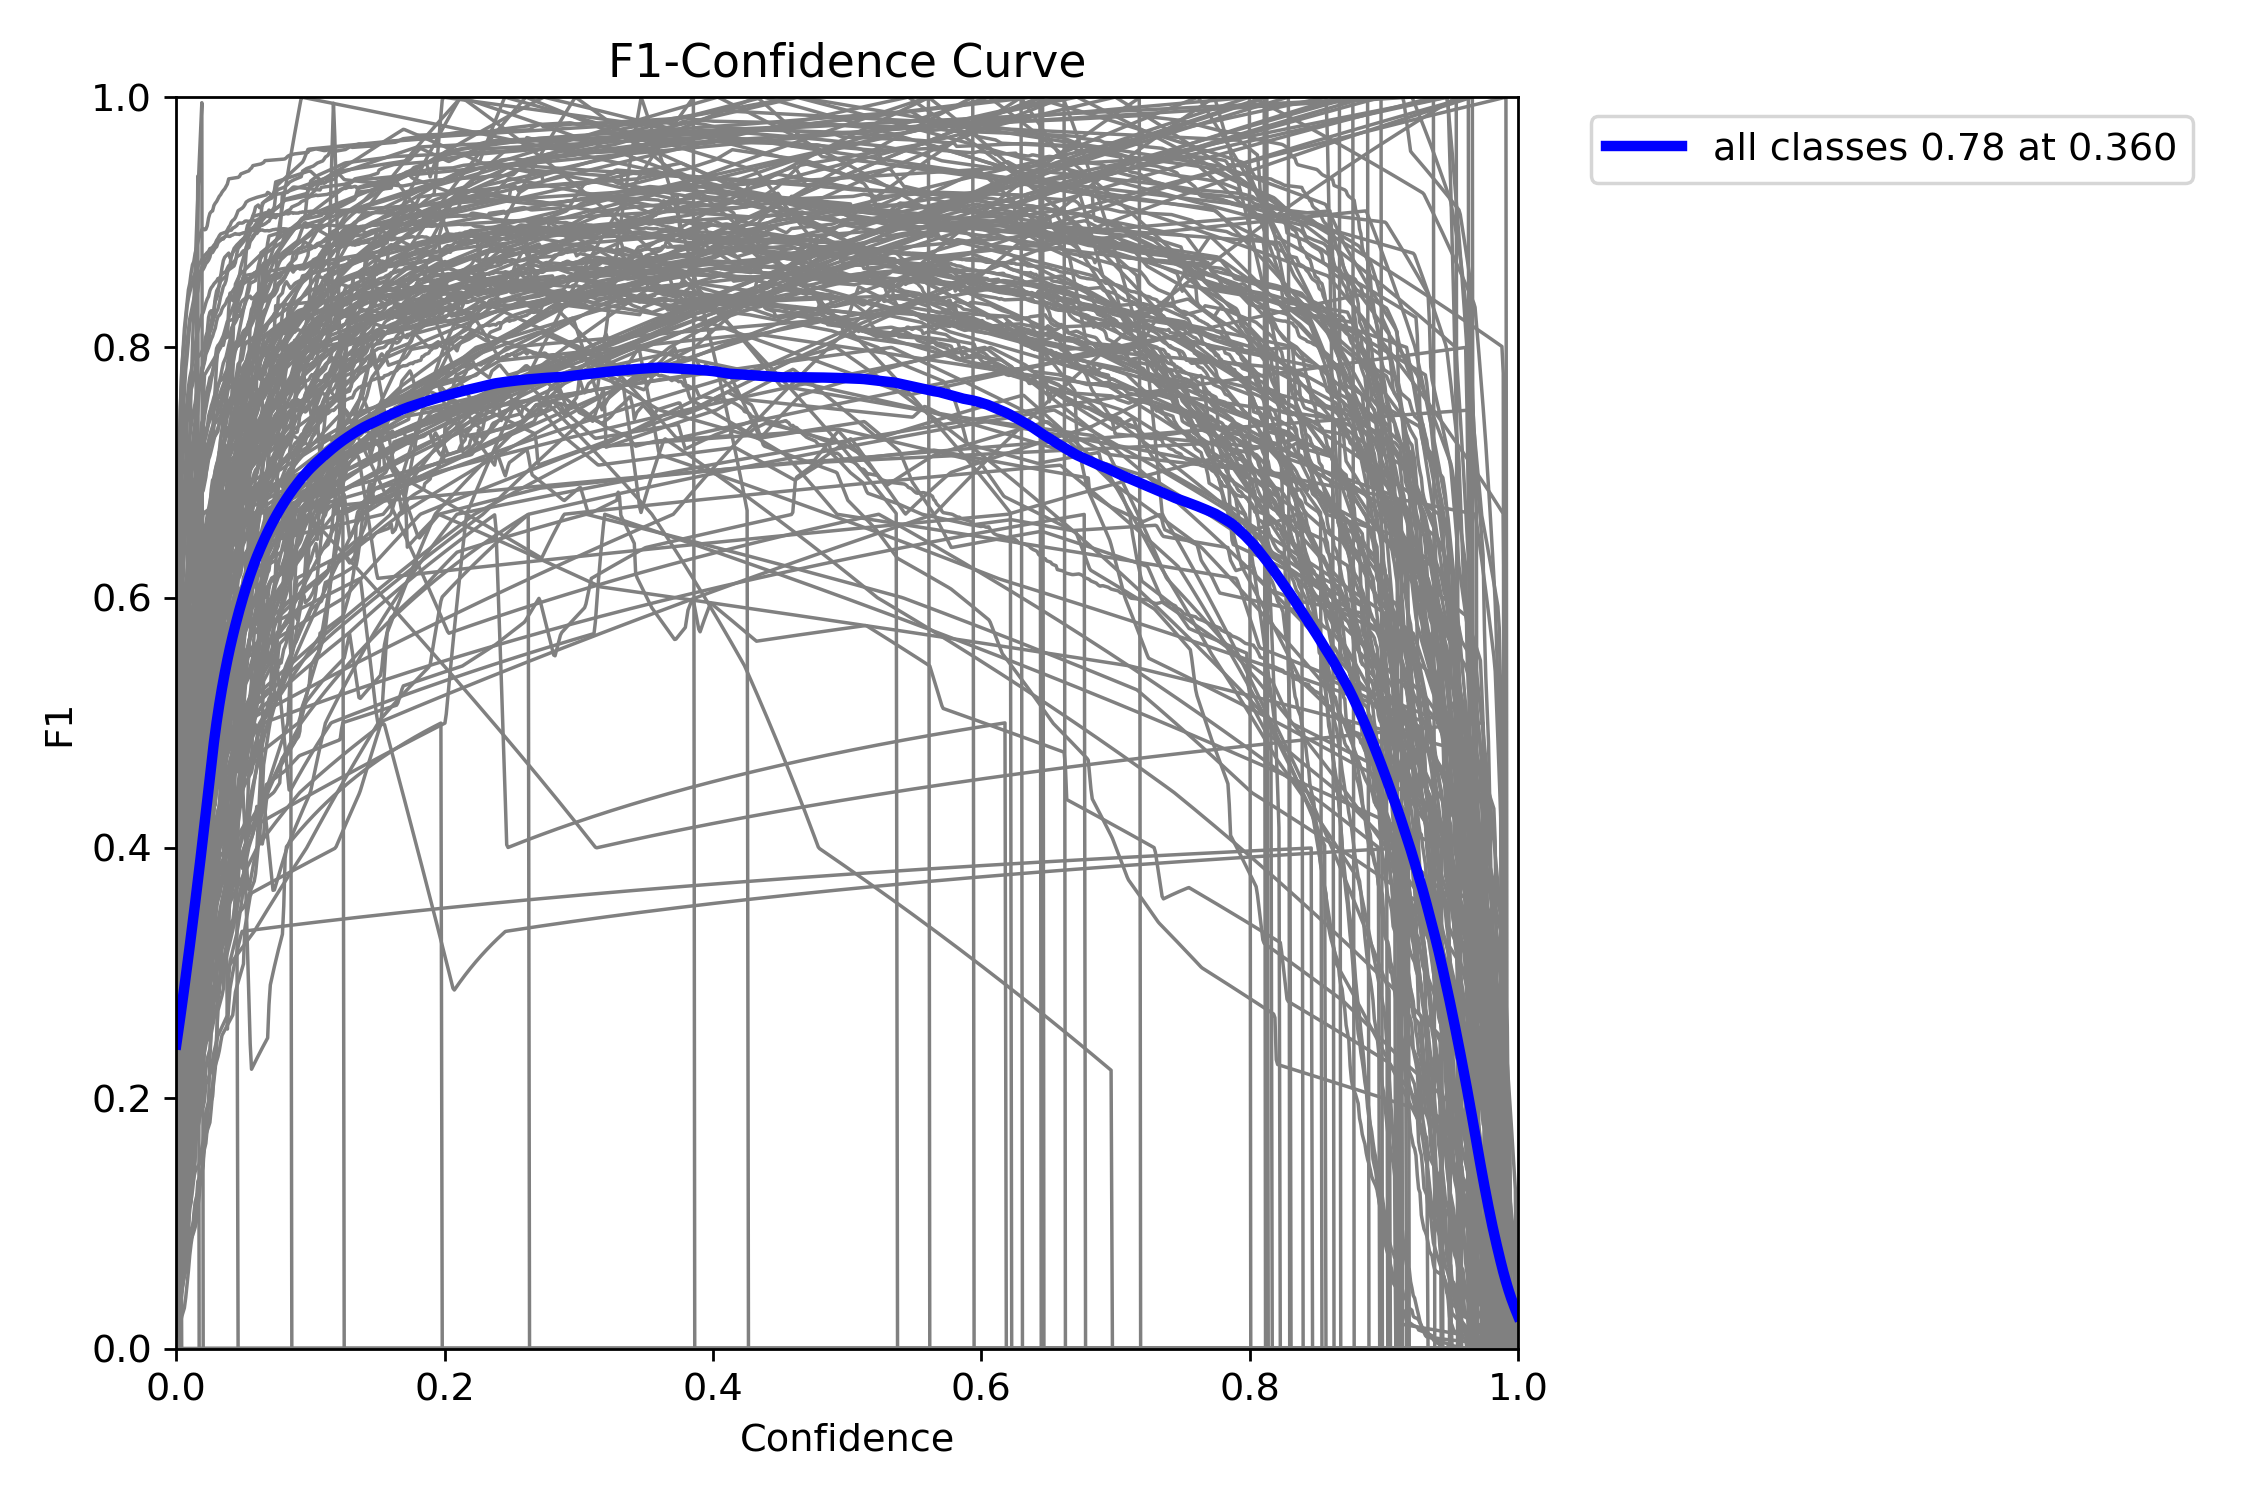
\includegraphics[width=0.4\textwidth]{../figure/tt100k_v11s_F1_curve.png}
        } \\
        \subfloat[YOLOv10s\label{fig:tt100k_10s_f1}]{
            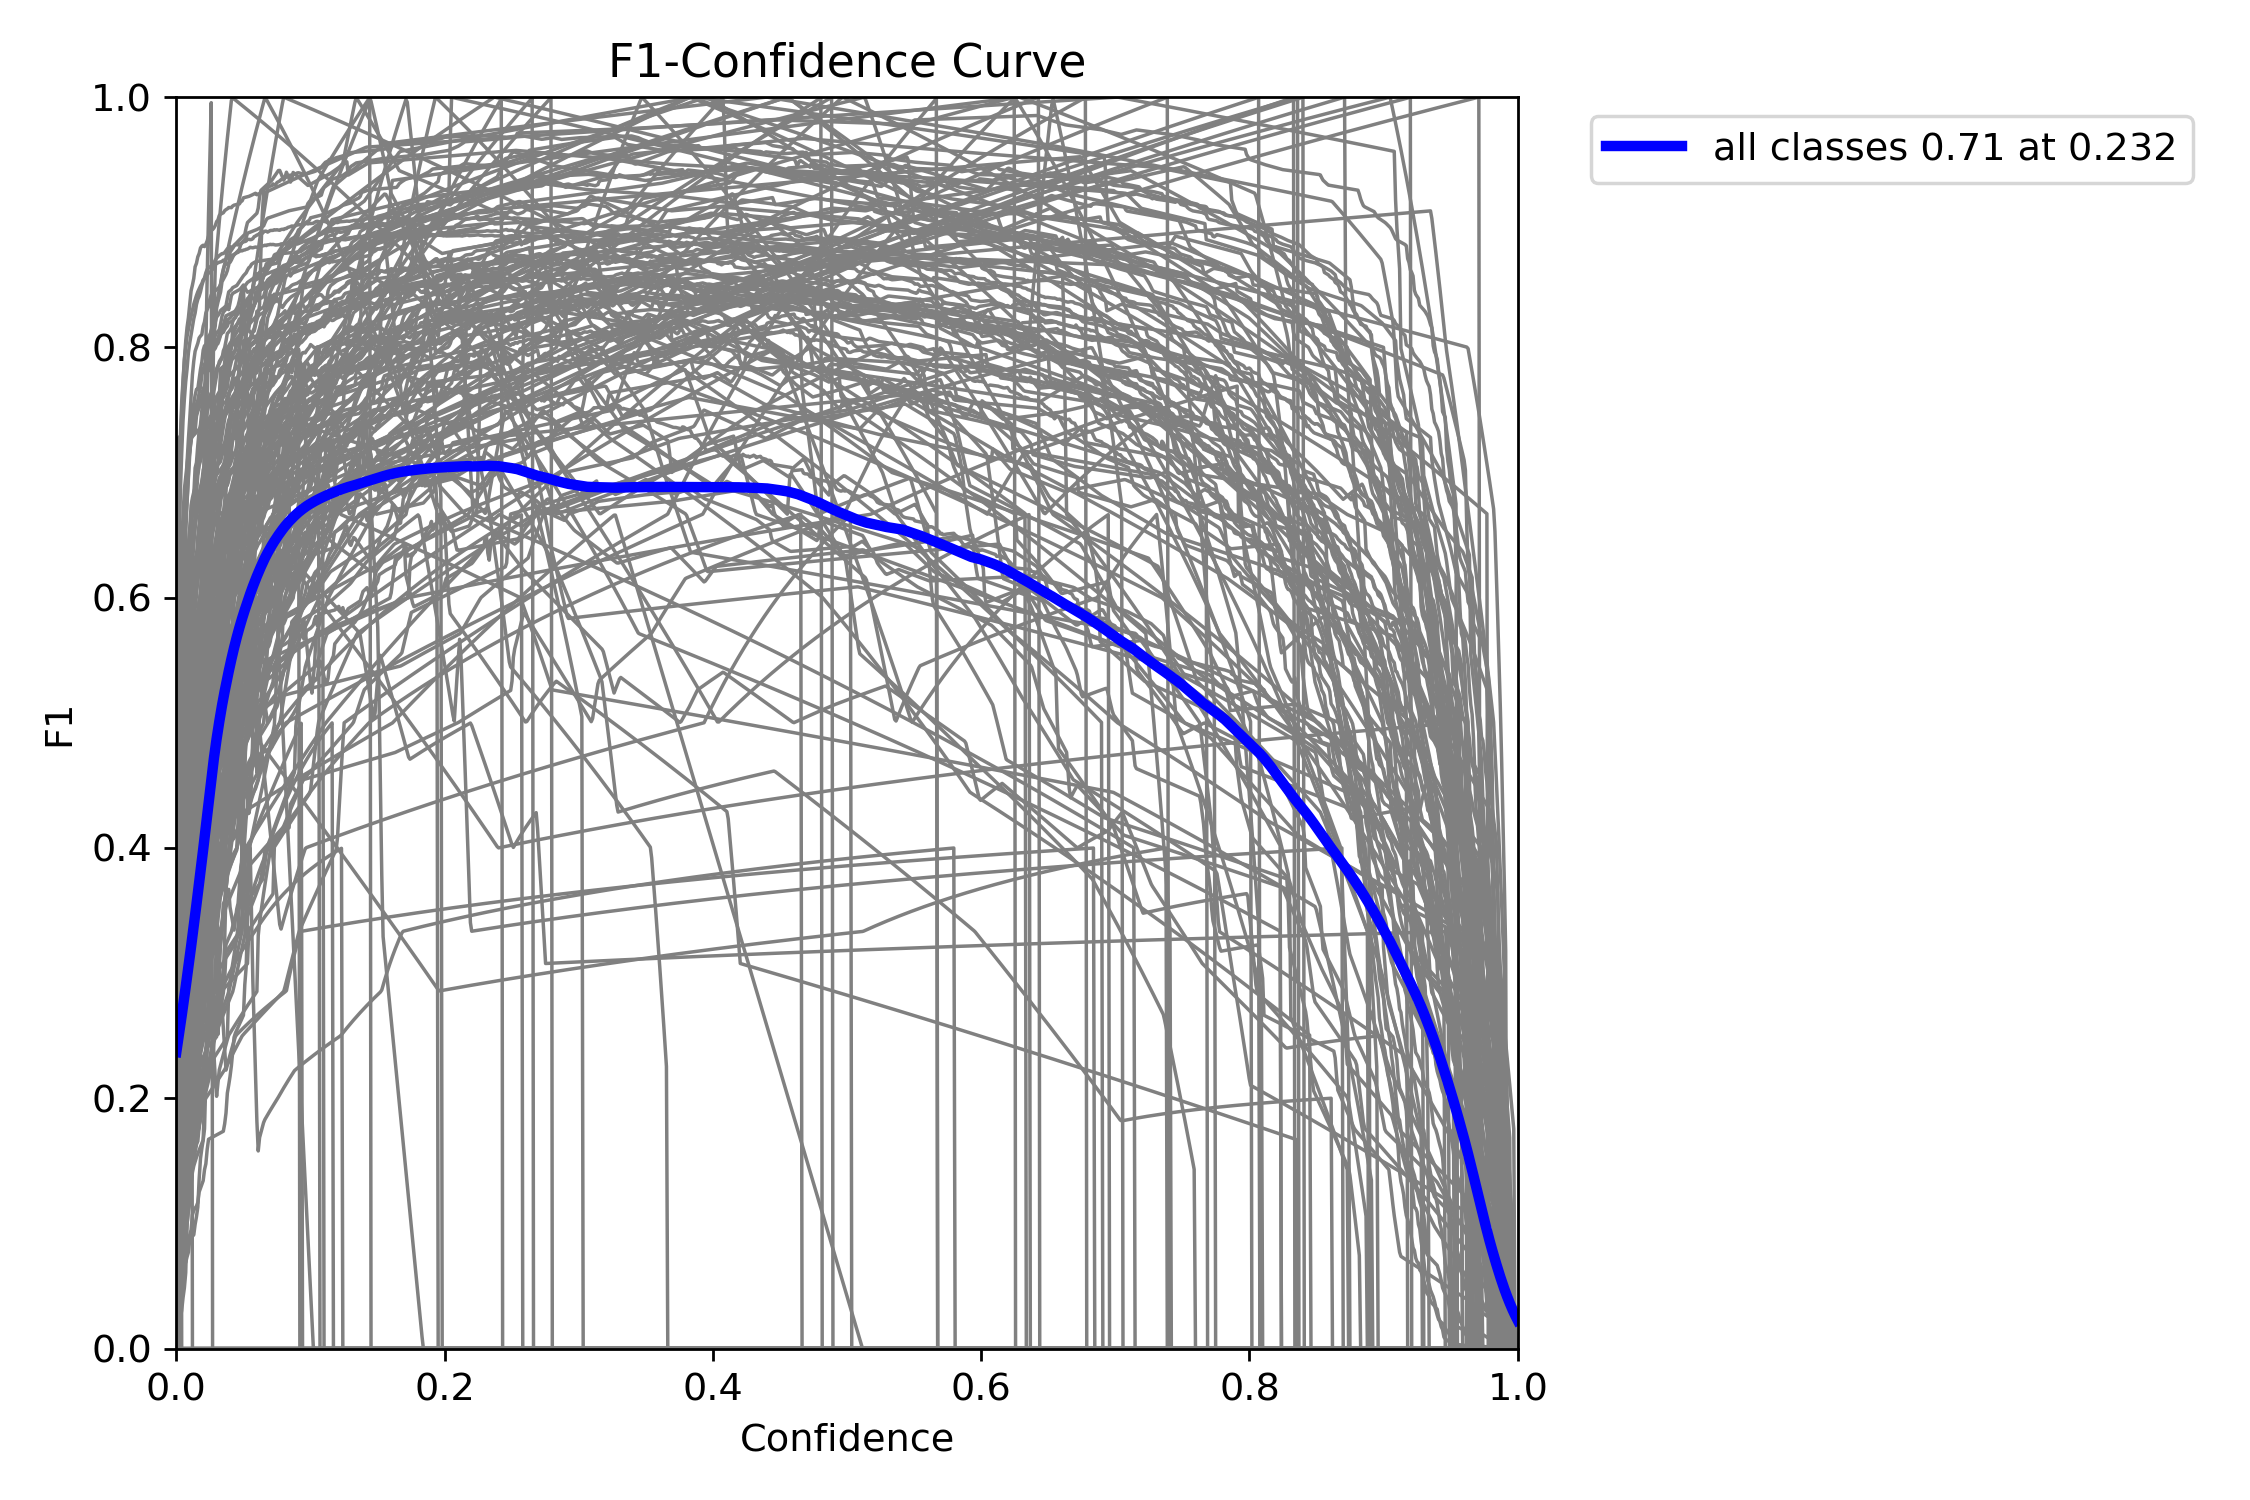
\includegraphics[width=0.4\textwidth]{../figure/tt100k_v10s_F1_curve.png}
        }
        \subfloat[YOLOv9s\label{fig:tt100k_9s_f1}]{
            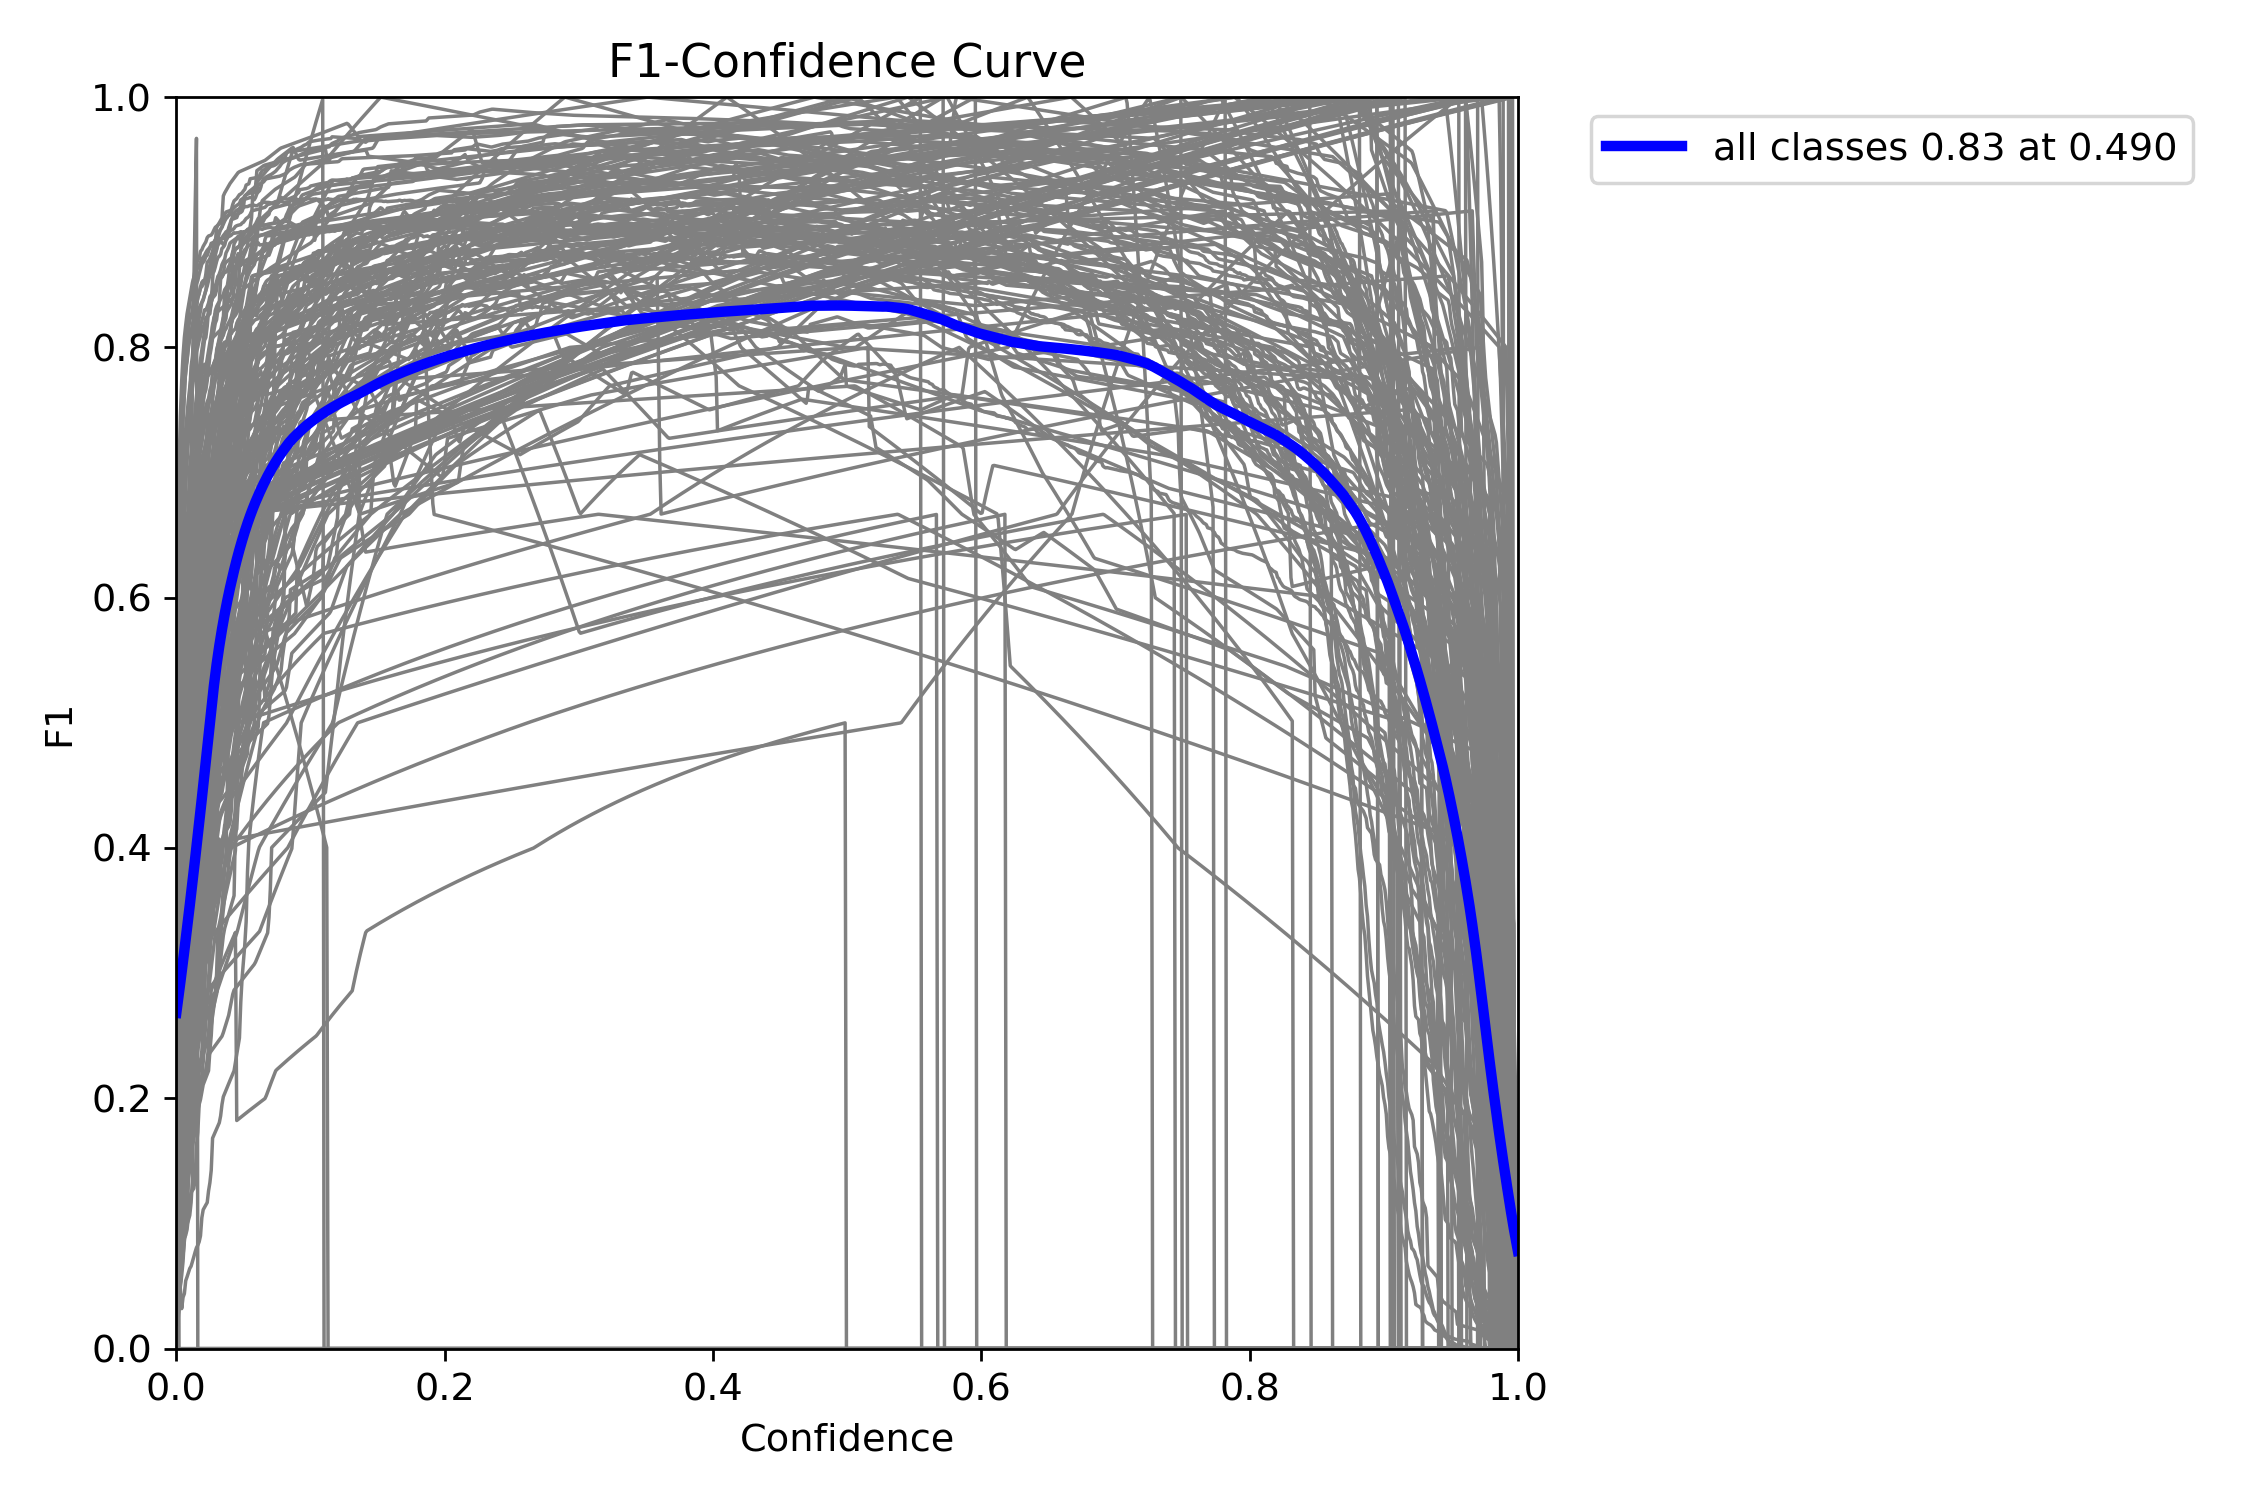
\includegraphics[width=0.4\textwidth]{../figure/tt100k_v9s_F1_curve.png}
        }
    \captionsetup{font=footnotesize}
    \bicaption{不同的网络模型在TT100K数据集上的F1得分}{Symbol cross-reference table}
    \label{fig:tt100k_f1}
\end{figure}

在表 \ref{tab:compare_studies_tt100k} 中,从模型参数来看,YOLOv9s参数容量是最小的,只有7.5MB,而改进后的模型参数容量相对较大,为11.4MB。
虽然our 模型在参数方面有所增加,但在计算量(GFLOP)方面显示出显著优势。
它的计算量只有17.0GFLOPs,远远低于YOLOv11s的21.8GFLOPs、YOLOv10s的25.4GFLOPs和YOLOv9s的27.2GFLOPs。
这表明our 模型在设计中更加关注计算效率。
通过优化算法结构和引入高效模块,它有效地降低了模型的计算复杂性。

在精度(P)方面,YOLOv9s表现最好,为0.914,our 模型为0.875,略低于YOLOv11s的0.878,但高于YOLOv10s的0.776。
在召回(R)方面,our 模型达到了0.830,高于0.777的YOLOv11s、0.752的YOLOv10s和0.818的YOLOv9s。
在mAP性能方面,YOLOv9s以0.906的$mAP_{0.5}$领先,但our 模型紧随其后,达到0.893的$mAP_{0.5}$,明显高于YOLOv11s的0.877和YOLOv10s的0.850。
这表明our 模型在小型目标检测任务中具有很强的竞争力,这可以有效地提高无人机对交通标志等小型目标的检测精度。
虽然与YOLOv9s存在一定的差距,但考虑到我们模型的计算量大幅减少,这种差距在实际应用中是可以接受的,our 模型在精度和效率之间实现了良好的平衡。

图 \ref{fig:tt100k_cmn} 呈现了 YOLOv9s、YOLOv10s、YOLOv11s 以及 our 模型在TT100K数据集针对不同类别目标的预测状况。具体而言,图 \ref{fig:tt100k_cmn} 为归一化混淆矩阵的热力图形式,其中颜色深浅与预测概率呈正相关,颜色愈深,意味着预测准确率愈高,相应地,颜色愈浅,则表明预测准确率较低。需要强调的是,热力图对角线上的数据对应着模型成功预测正确标签的情况,而非对角线部分的数据则反映了模型出现标签预测错误的情形。

然而,从直观观察的角度来看,图 \ref{fig:tt100k_ex_cmn}、图 \ref{fig:tt100k_11s_cmn}、图 \ref{fig:tt100k_10s_cmn} 以及图 \ref{fig:tt100k_9s_cmn} 均难以清晰地辨识出每一个类别具体的预测数据细节。但深入分析可发现,于图 \ref{fig:tt100k_ex_cmn} 所示的 our 模型中,预测错误标签几率超过 0.5 的类别数量为 7 个;在图 \ref{fig:tt100k_11s_cmn} 展示的 YOLOv11s 模型里,这一数值同样为 7 个;从图 \ref{fig:tt100k_10s_cmn} 可知,在 YOLOv10s 模型中,预测错误标签几率大于 0.5 的类别有 9 个;而依据图 \ref{fig:tt100k_9s_cmn},YOLOv9s 模型中预测错误标签几率大于 0.5 的类别数量为 4 个。

综合图 \ref{fig:tt100k_cmn} 所揭示的归一化混淆矩阵热力图信息,可以明确地得出结论:在 TT100K 数据集上,YOLOv9s 模型在预测正确类别方面展现出更为卓越的性能,这一结论也得到了表 \ref{tab:compare_studies_tt100k} 中相关数据的有力印证 ——YOLOv9s 的精确度和召回率分别达到了 0.914 和 0.818。尽管 our 模型在预测正确标签的性能上稍逊于 YOLOv9s 模型,但与 YOLOv11s 模型相比,our 模型在预测正确标签方面维持了相近的性能水平,且二者的表现均优于 YOLOv10s 模型。

FPS受到硬件的极大影响,但就相对价值而言,我们模型的FPS为84.7,低于94.3的YOLOv11s、88.5的YOLOv10s和90.9的YOLOv9。 这主要是由于在our 模型中引入SPPC模块和DSC模块后,模型参数的增加,导致计算量相对较大,从而影响了处理速度。 然而,在实际应用中,FPS的差异并不大,our 模型仍然可以通过优化计算量,同时确保高检测性能,在一定程度上满足无人机实时检测的需求。

图 \ref{fig:tt100k_f1} 展示了不同模型的F1得分曲线。YOLOv9s的mAP是最高的(0.906),这与其高F1 AUC一致。 我们模型的mAP为0.893,略低于YOLOv9s,但高于YOLOv11s和YOLOv10s。 这表明,尽管our 模型在平均精度上略低于YOLOv9s,但不同F1分数级别的综合性能与YOLOv9s非常接近。 F1曲线的高性能与我们模型的精度和召回率之间的良好平衡有关。 虽然F1曲线的性能略低于YOLOv9s,但our 模型仍然保持了高检测精度和处理速度,同时降低了计算量,这使得它在无人机的小目标检测任务中具有很高的实际应用价值。

\begin{table}[htbp]
    \centering
    \captionsetup{font=footnotesize}
    \bicaption{在VisDrone数据集上的对比实验结果}{Symbol cross-reference table}
    \label{tab:compare_studies_vd}
    \begin{tabular}{p{0.13\textwidth}p{0.13\textwidth}p{0.19\textwidth}p{0.1\textwidth}p{0.07\textwidth}p{0.07\textwidth}p{0.07\textwidth}}
        \toprule
        模型       & 参数量 MB & 计算量 GFLOPs & $mAP_{0.5}$   & P     & R     & FPS \\ 
        \midrule
        YOLOv11s     & 9.4   & 21.3         & 0.383           & 0.485  & 0.381 & 82.6 \\
        YOLOv10s     & 8.0   & 24.5         & 0.390           & 0.501  & 0.380 & 78.1 \\
        YOLOv9s      & 7.2   & 26.7         & \textbf{0.402}           & 0.525  & 0.392 & 62.1 \\
        \textbf{our} & 11.4  & \textbf{15.4} & 0.390 & 0.514  & 0.372 & 68.5 \\
        \bottomrule
    \end{tabular}
\end{table}

\begin{figure}[htbp]
    \centering
        \subfloat[EX-YOLO\label{fig:vd_ex_cmn}]{
            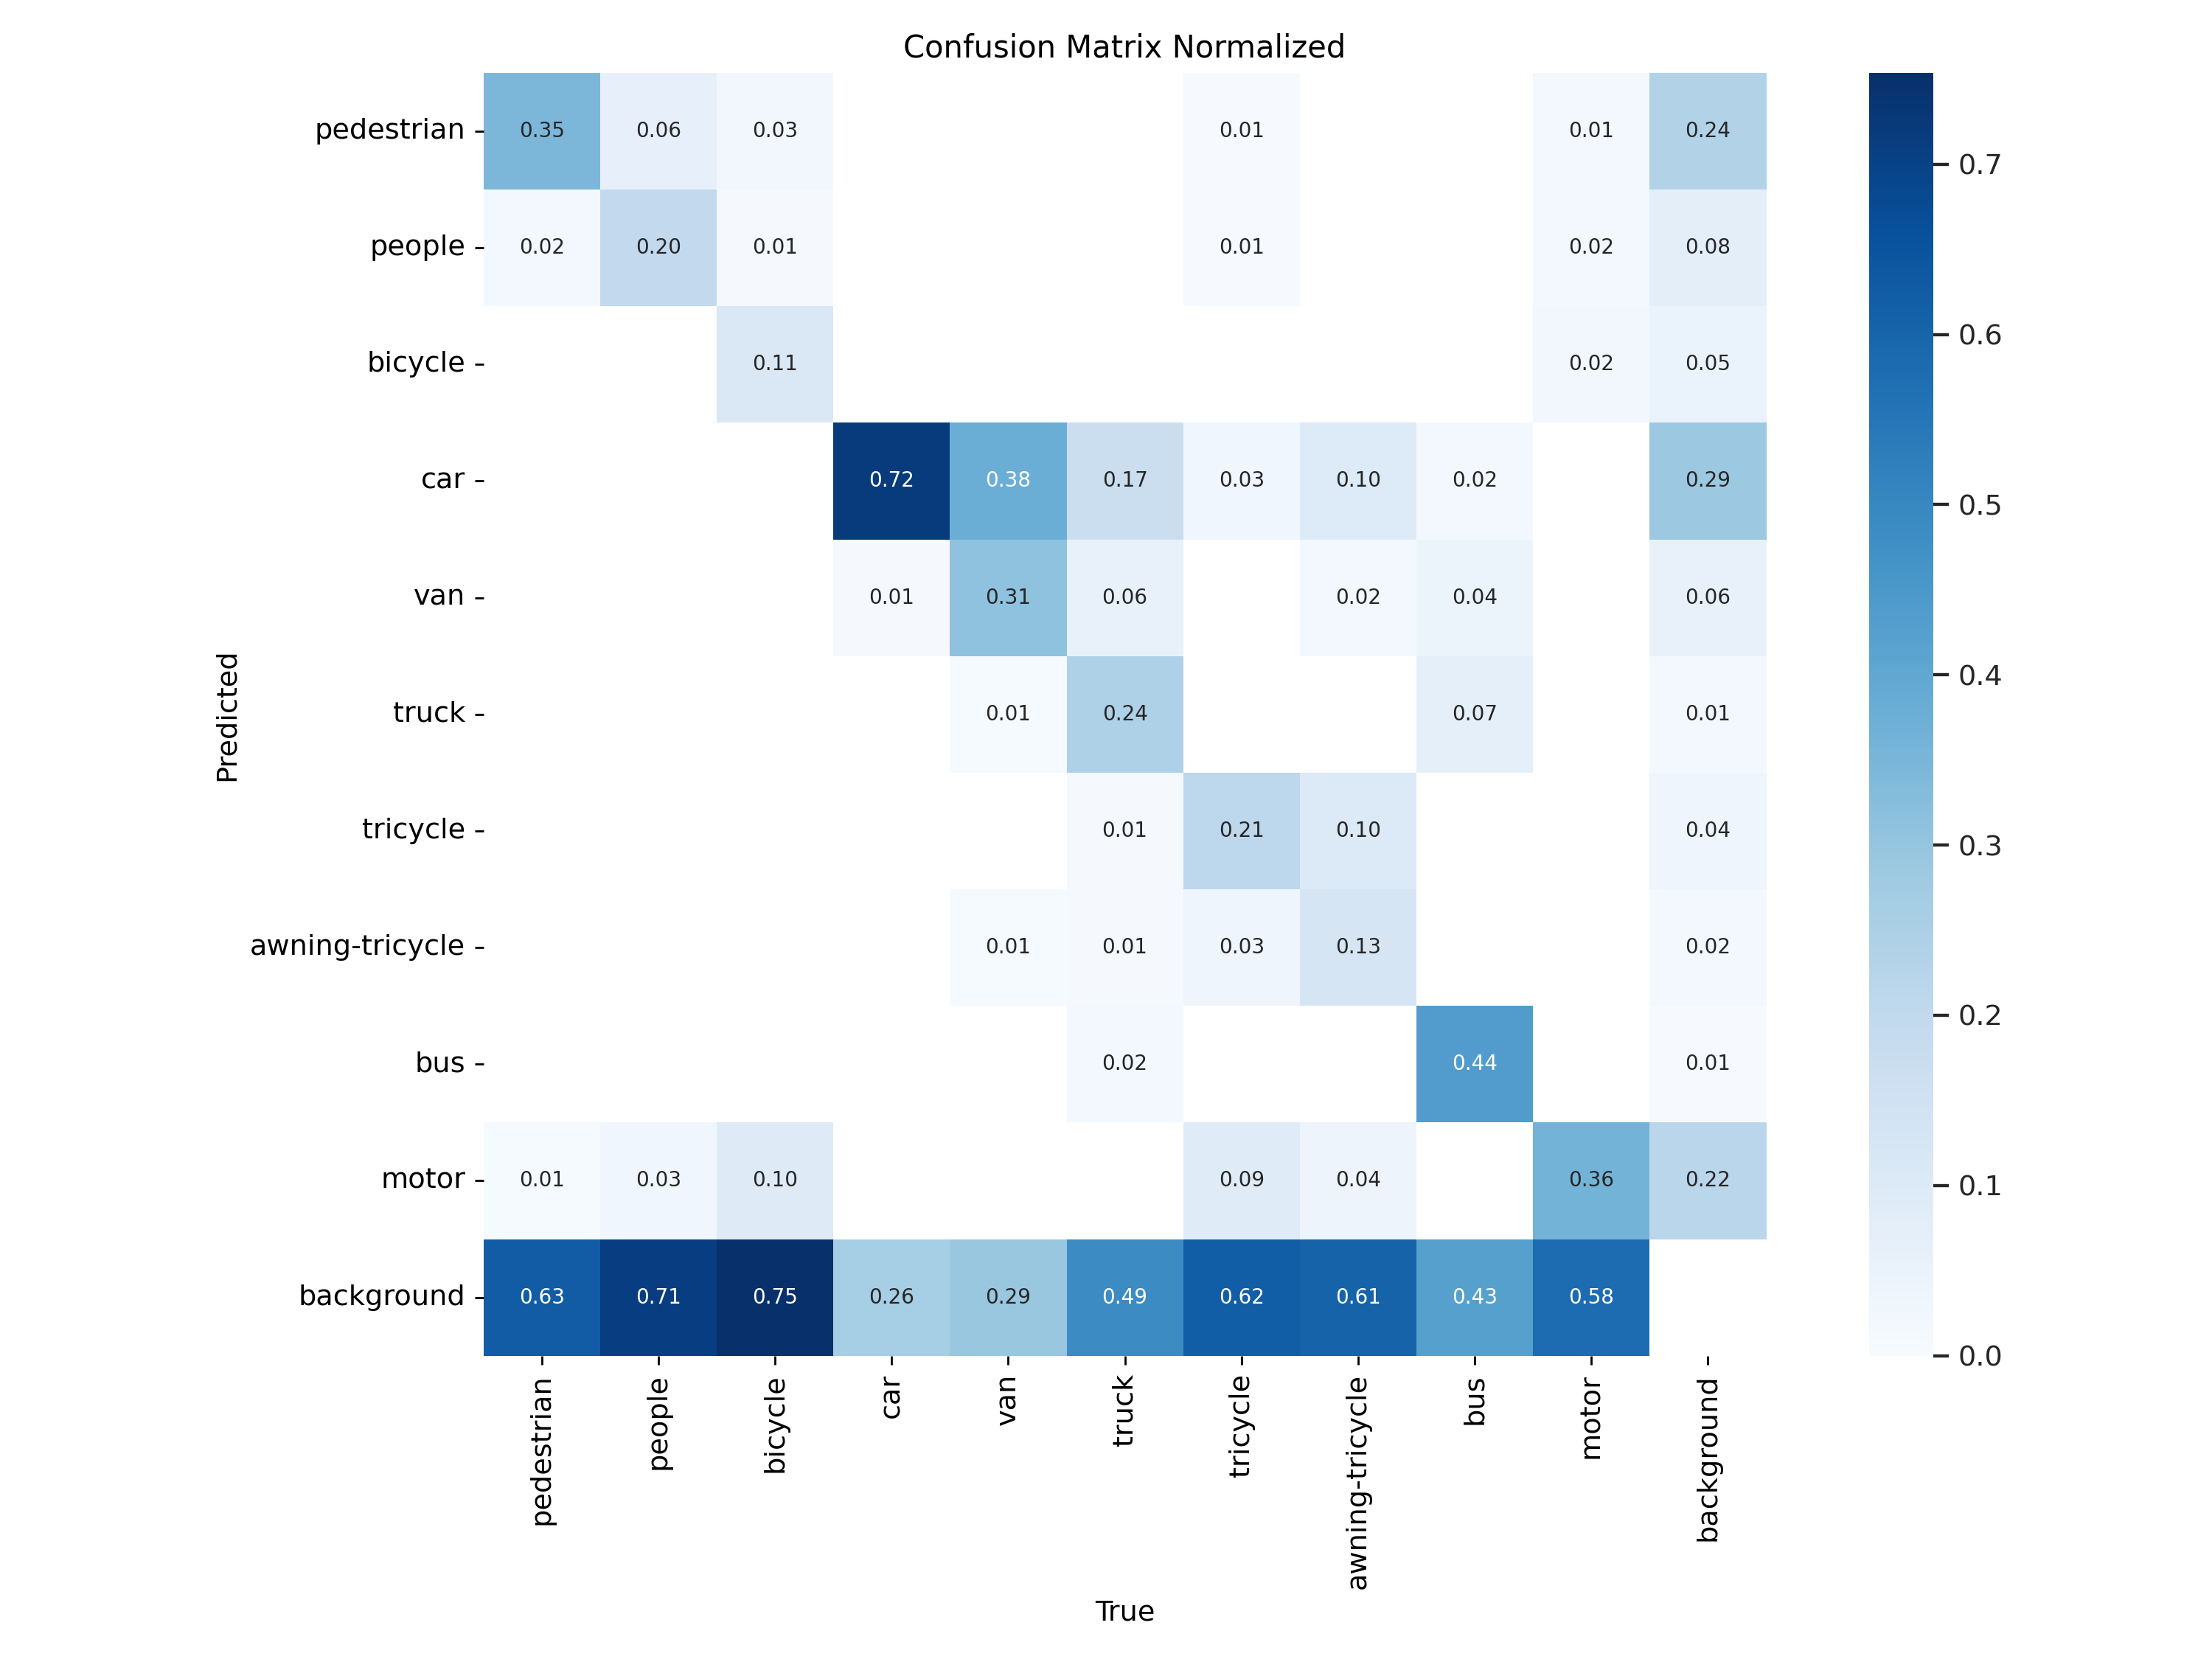
\includegraphics[width=0.4\textwidth]{../figure/vd_ex_confusion_matrix_normalized.png}
        }
        \subfloat[YOLOv11s\label{fig:vd_11s_cmn}]{
            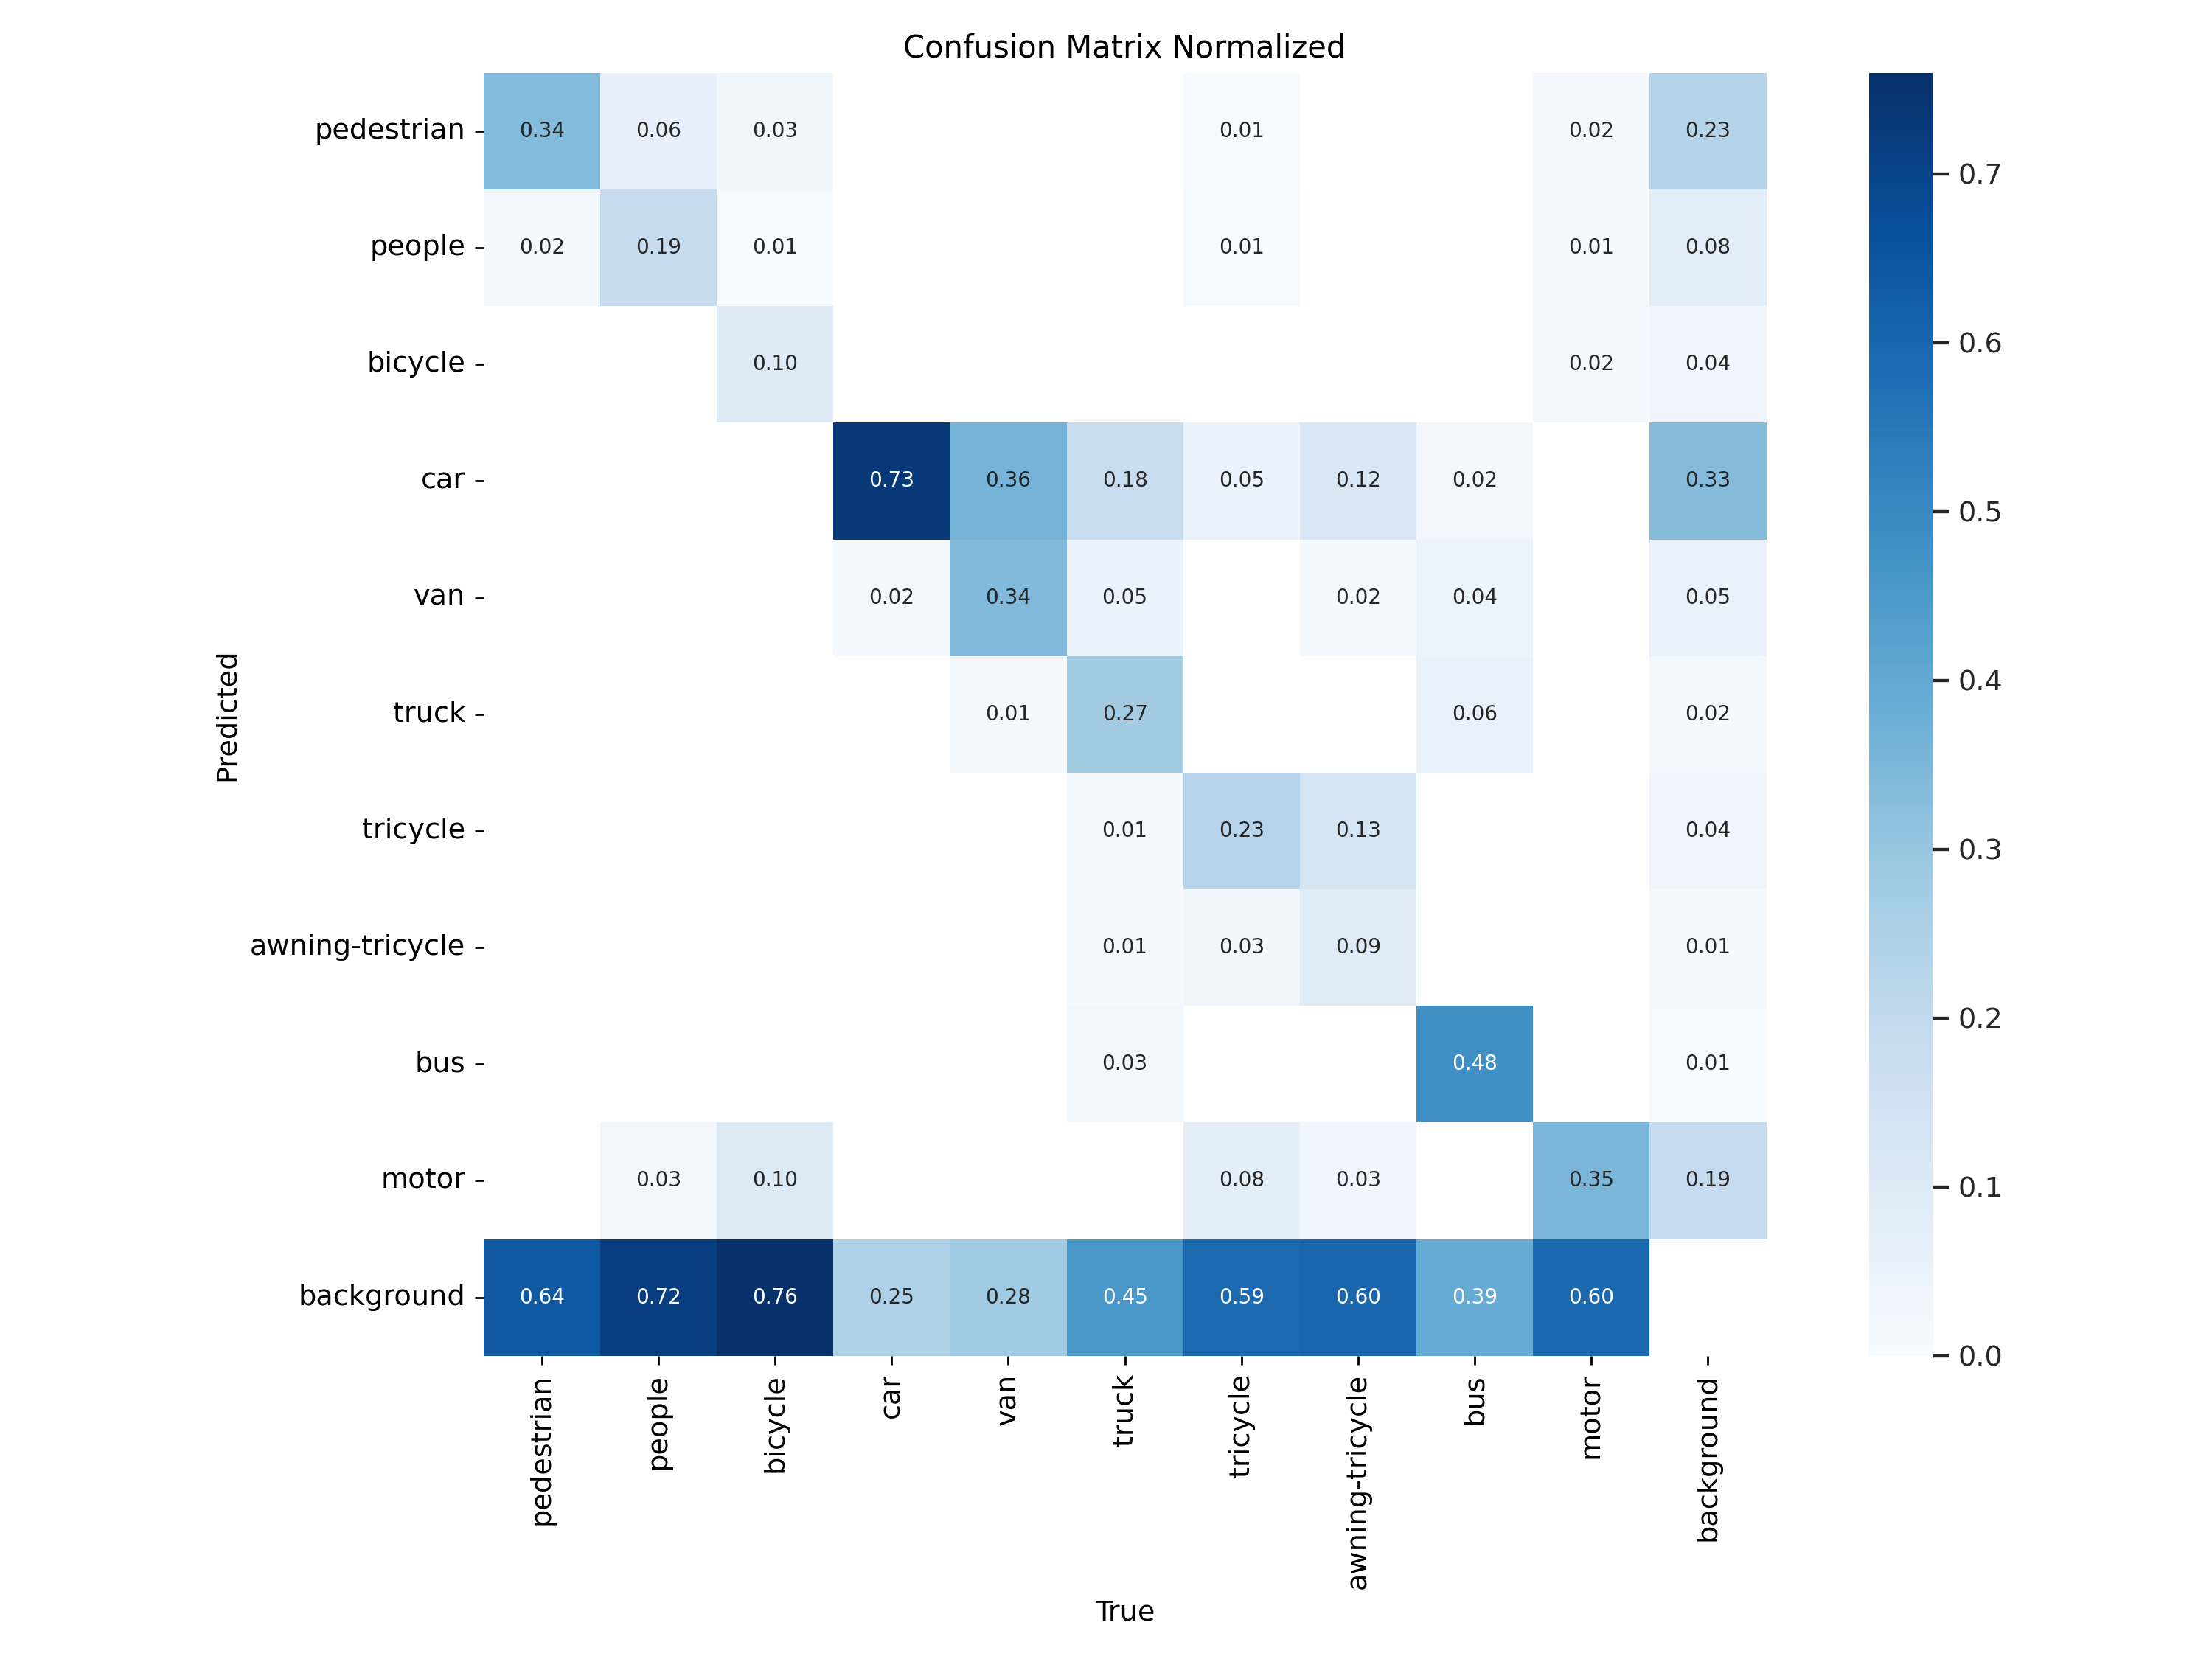
\includegraphics[width=0.4\textwidth]{../figure/vd_v11s_confusion_matrix_normalized.png}
        } \\
        \subfloat[YOLOv10s\label{fig:vd_10s_cmn}]{
            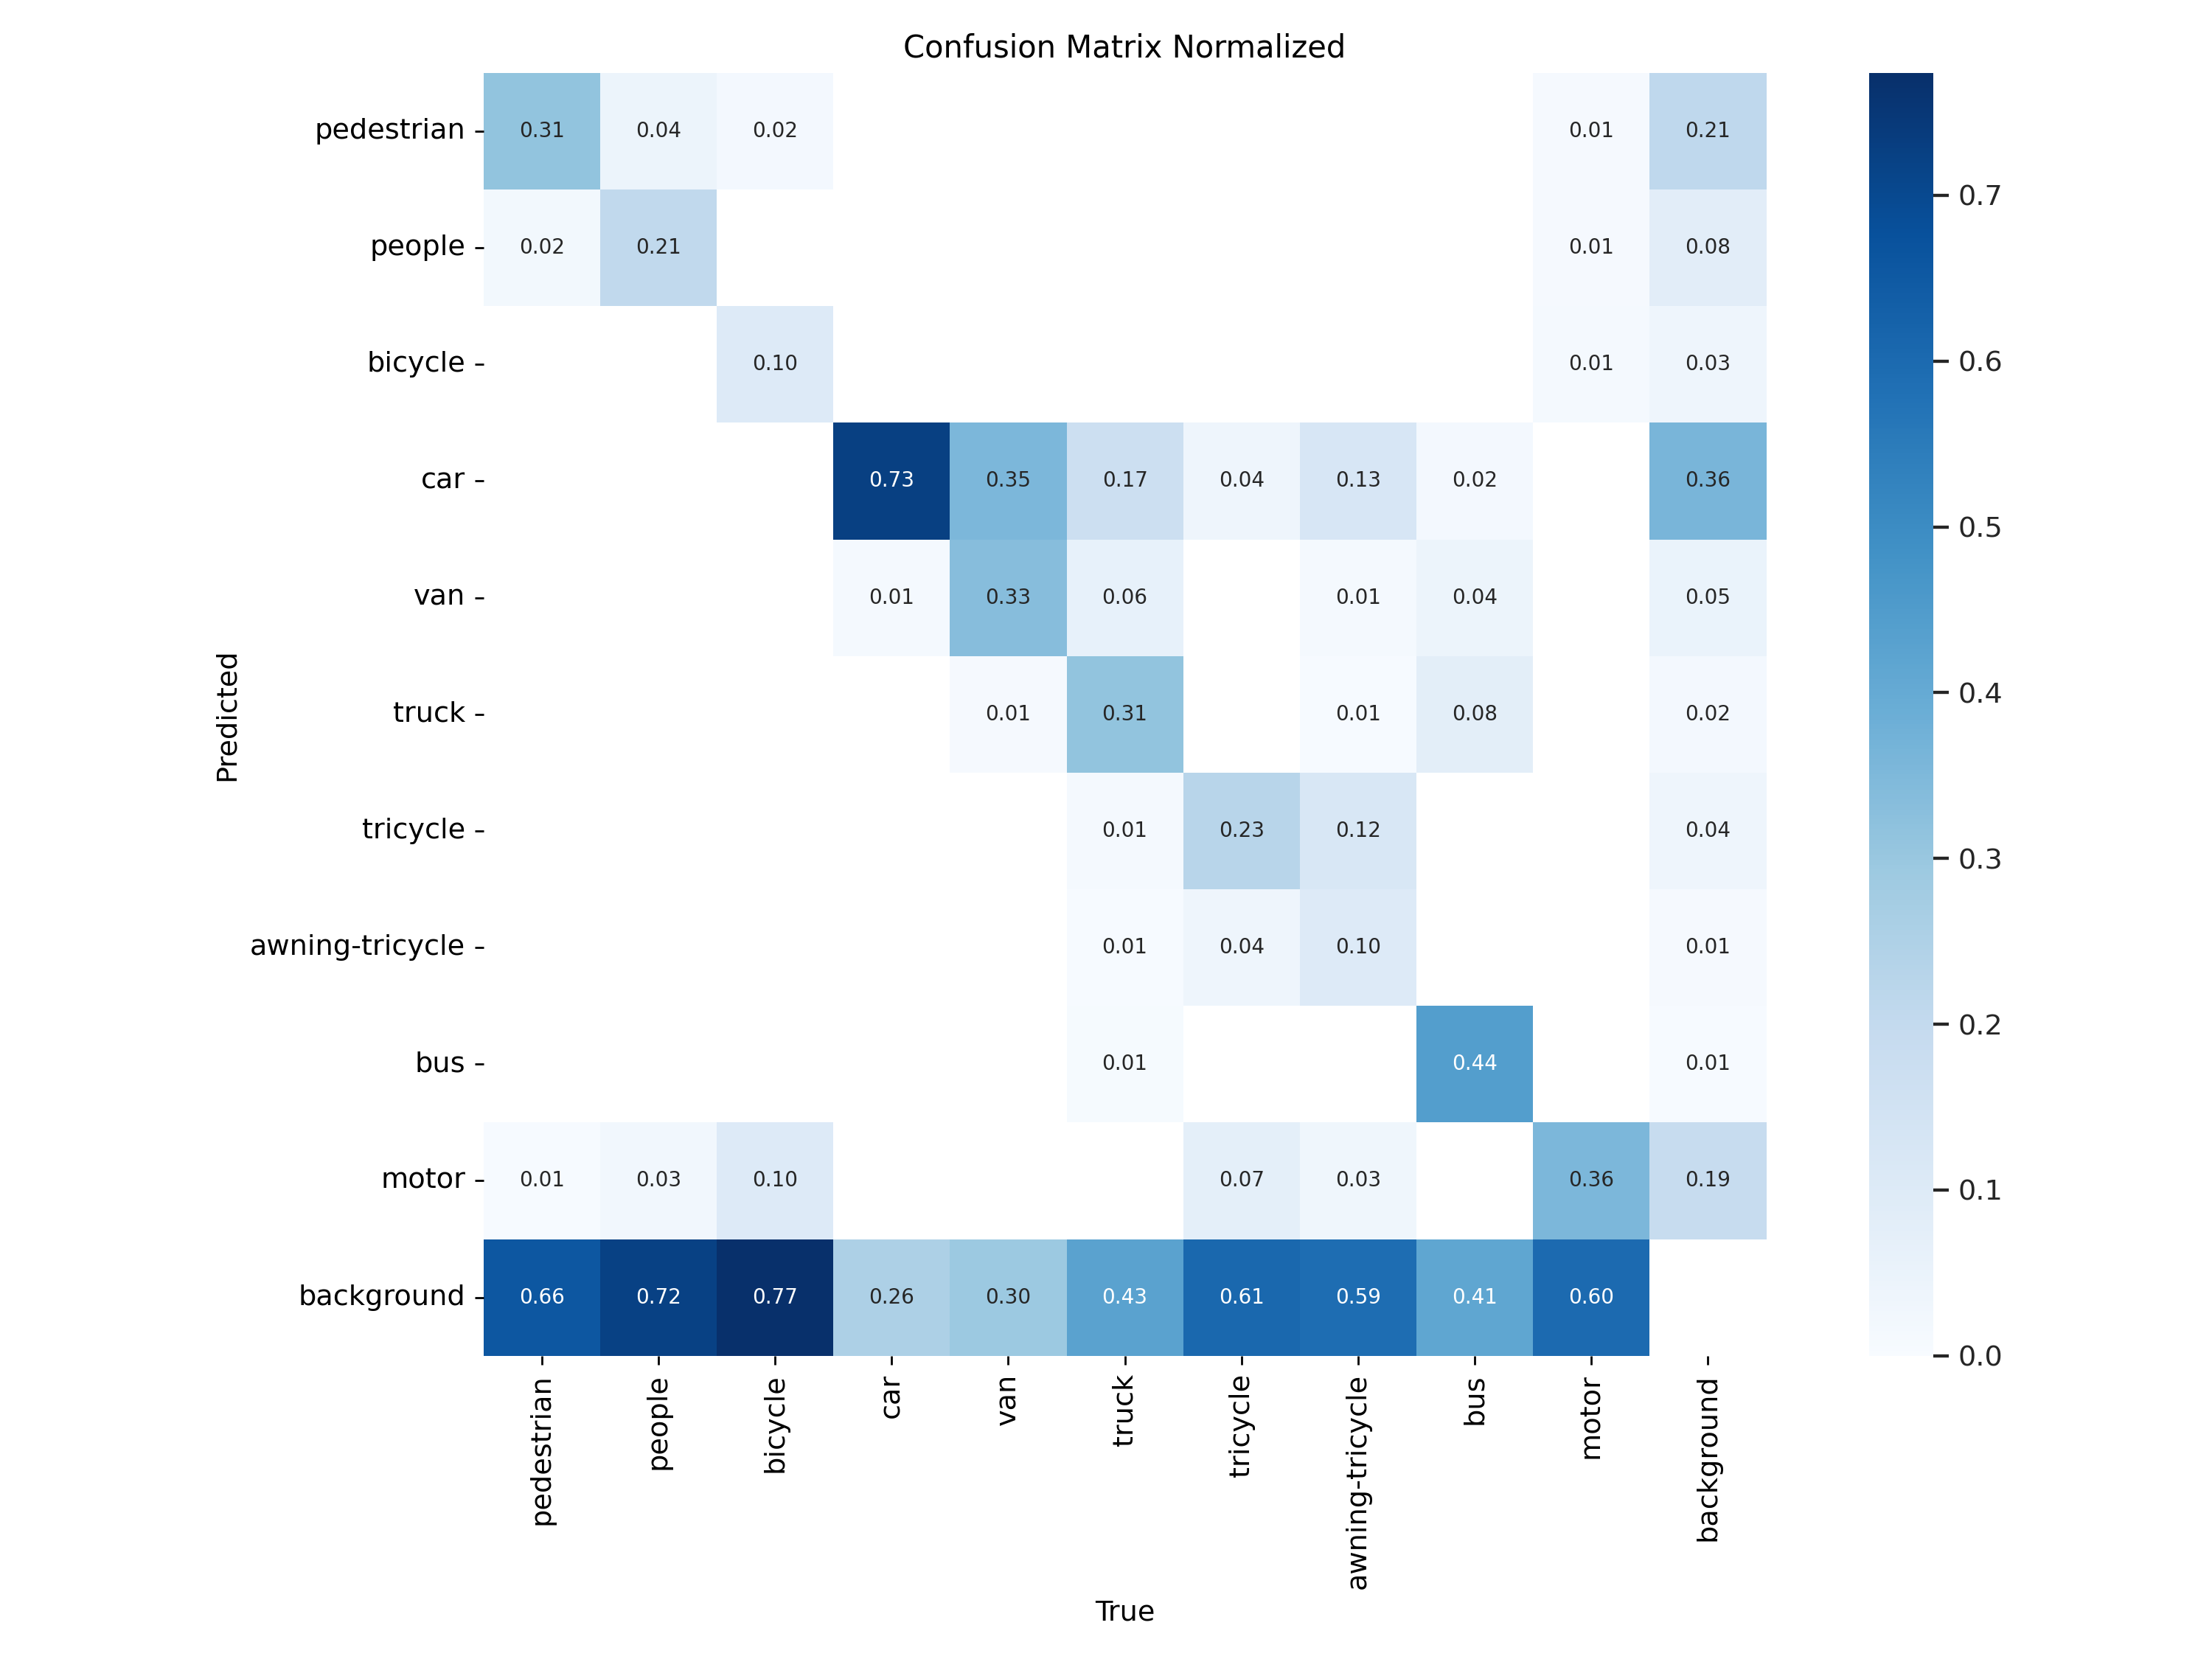
\includegraphics[width=0.4\textwidth]{../figure/vd_v10s_confusion_matrix_normalized.png}
        }
        \subfloat[YOLOv9s\label{fig:vd_9s_cmn}]{
            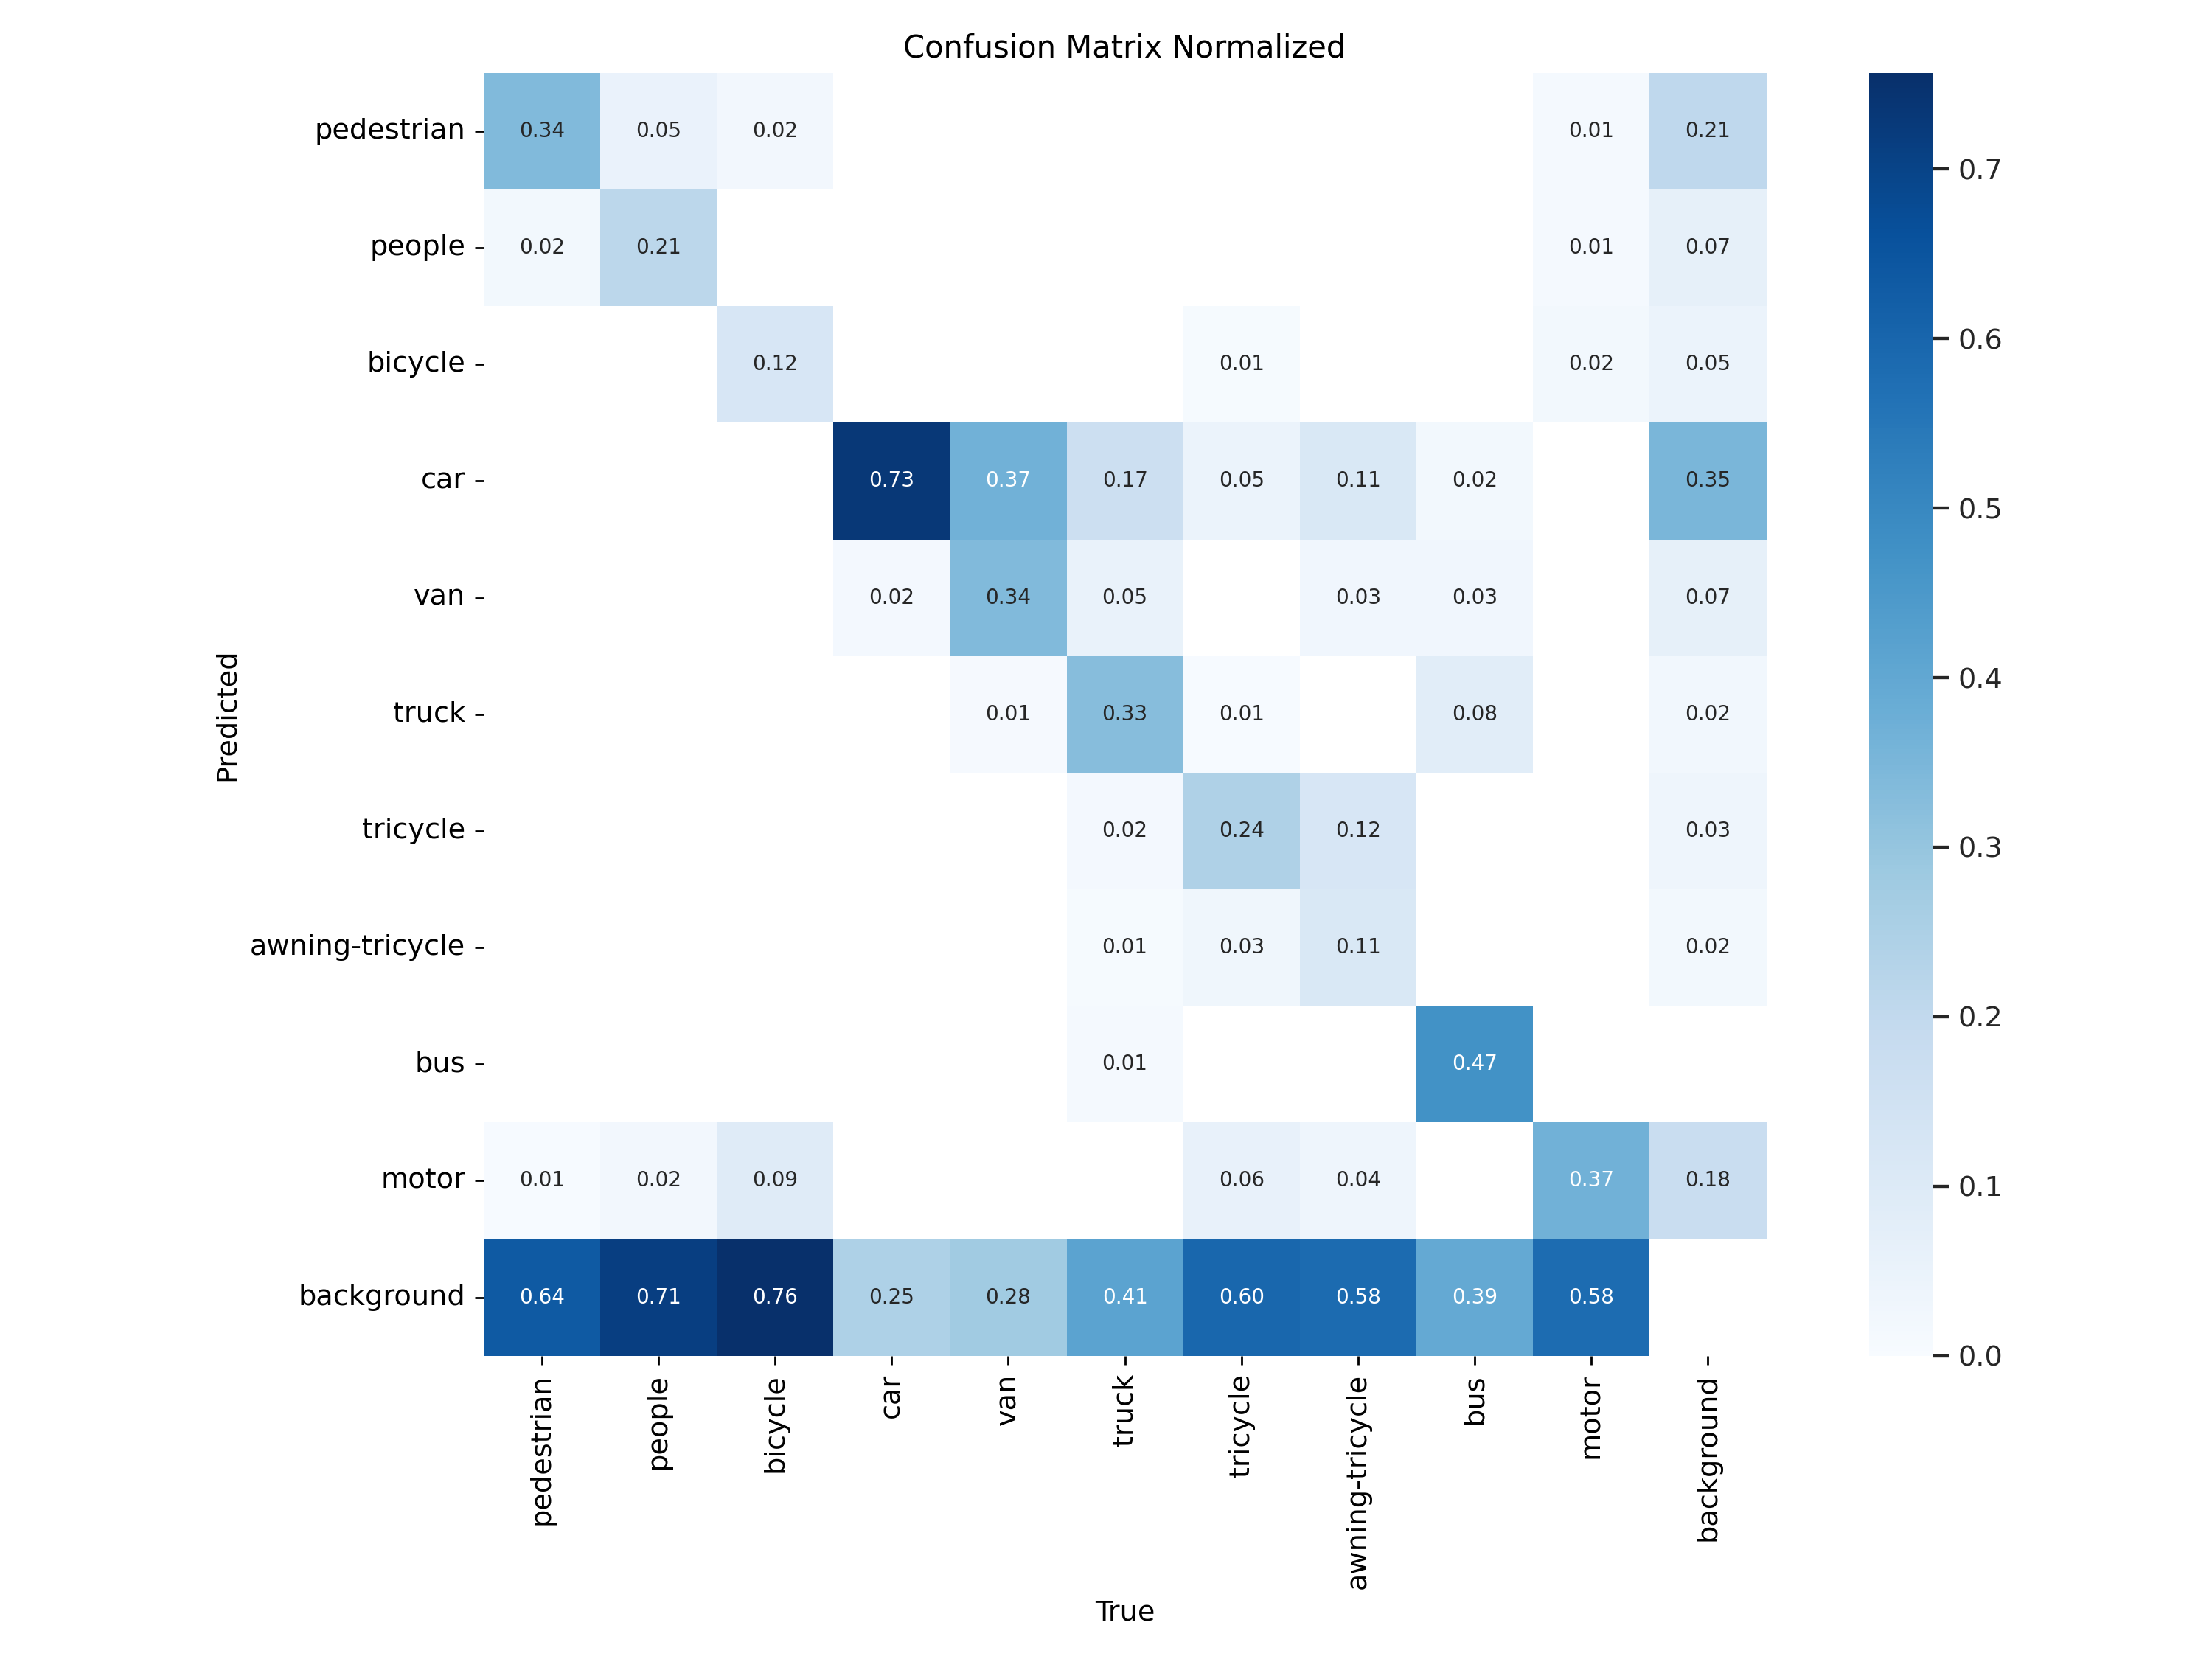
\includegraphics[width=0.4\textwidth]{../figure/vd_v9s_confusion_matrix_normalized.png}
        }
    \captionsetup{font=footnotesize}
    \bicaption{不同的网络模型在VisDrone数据集上的归一化混淆矩阵}{Symbol cross-reference table}
    \label{fig:vd_cmn}
\end{figure}

\begin{figure}[htbp]
    \centering
    \subfloat[EX-YOLO\label{fig:vd_ex_f1}]{
        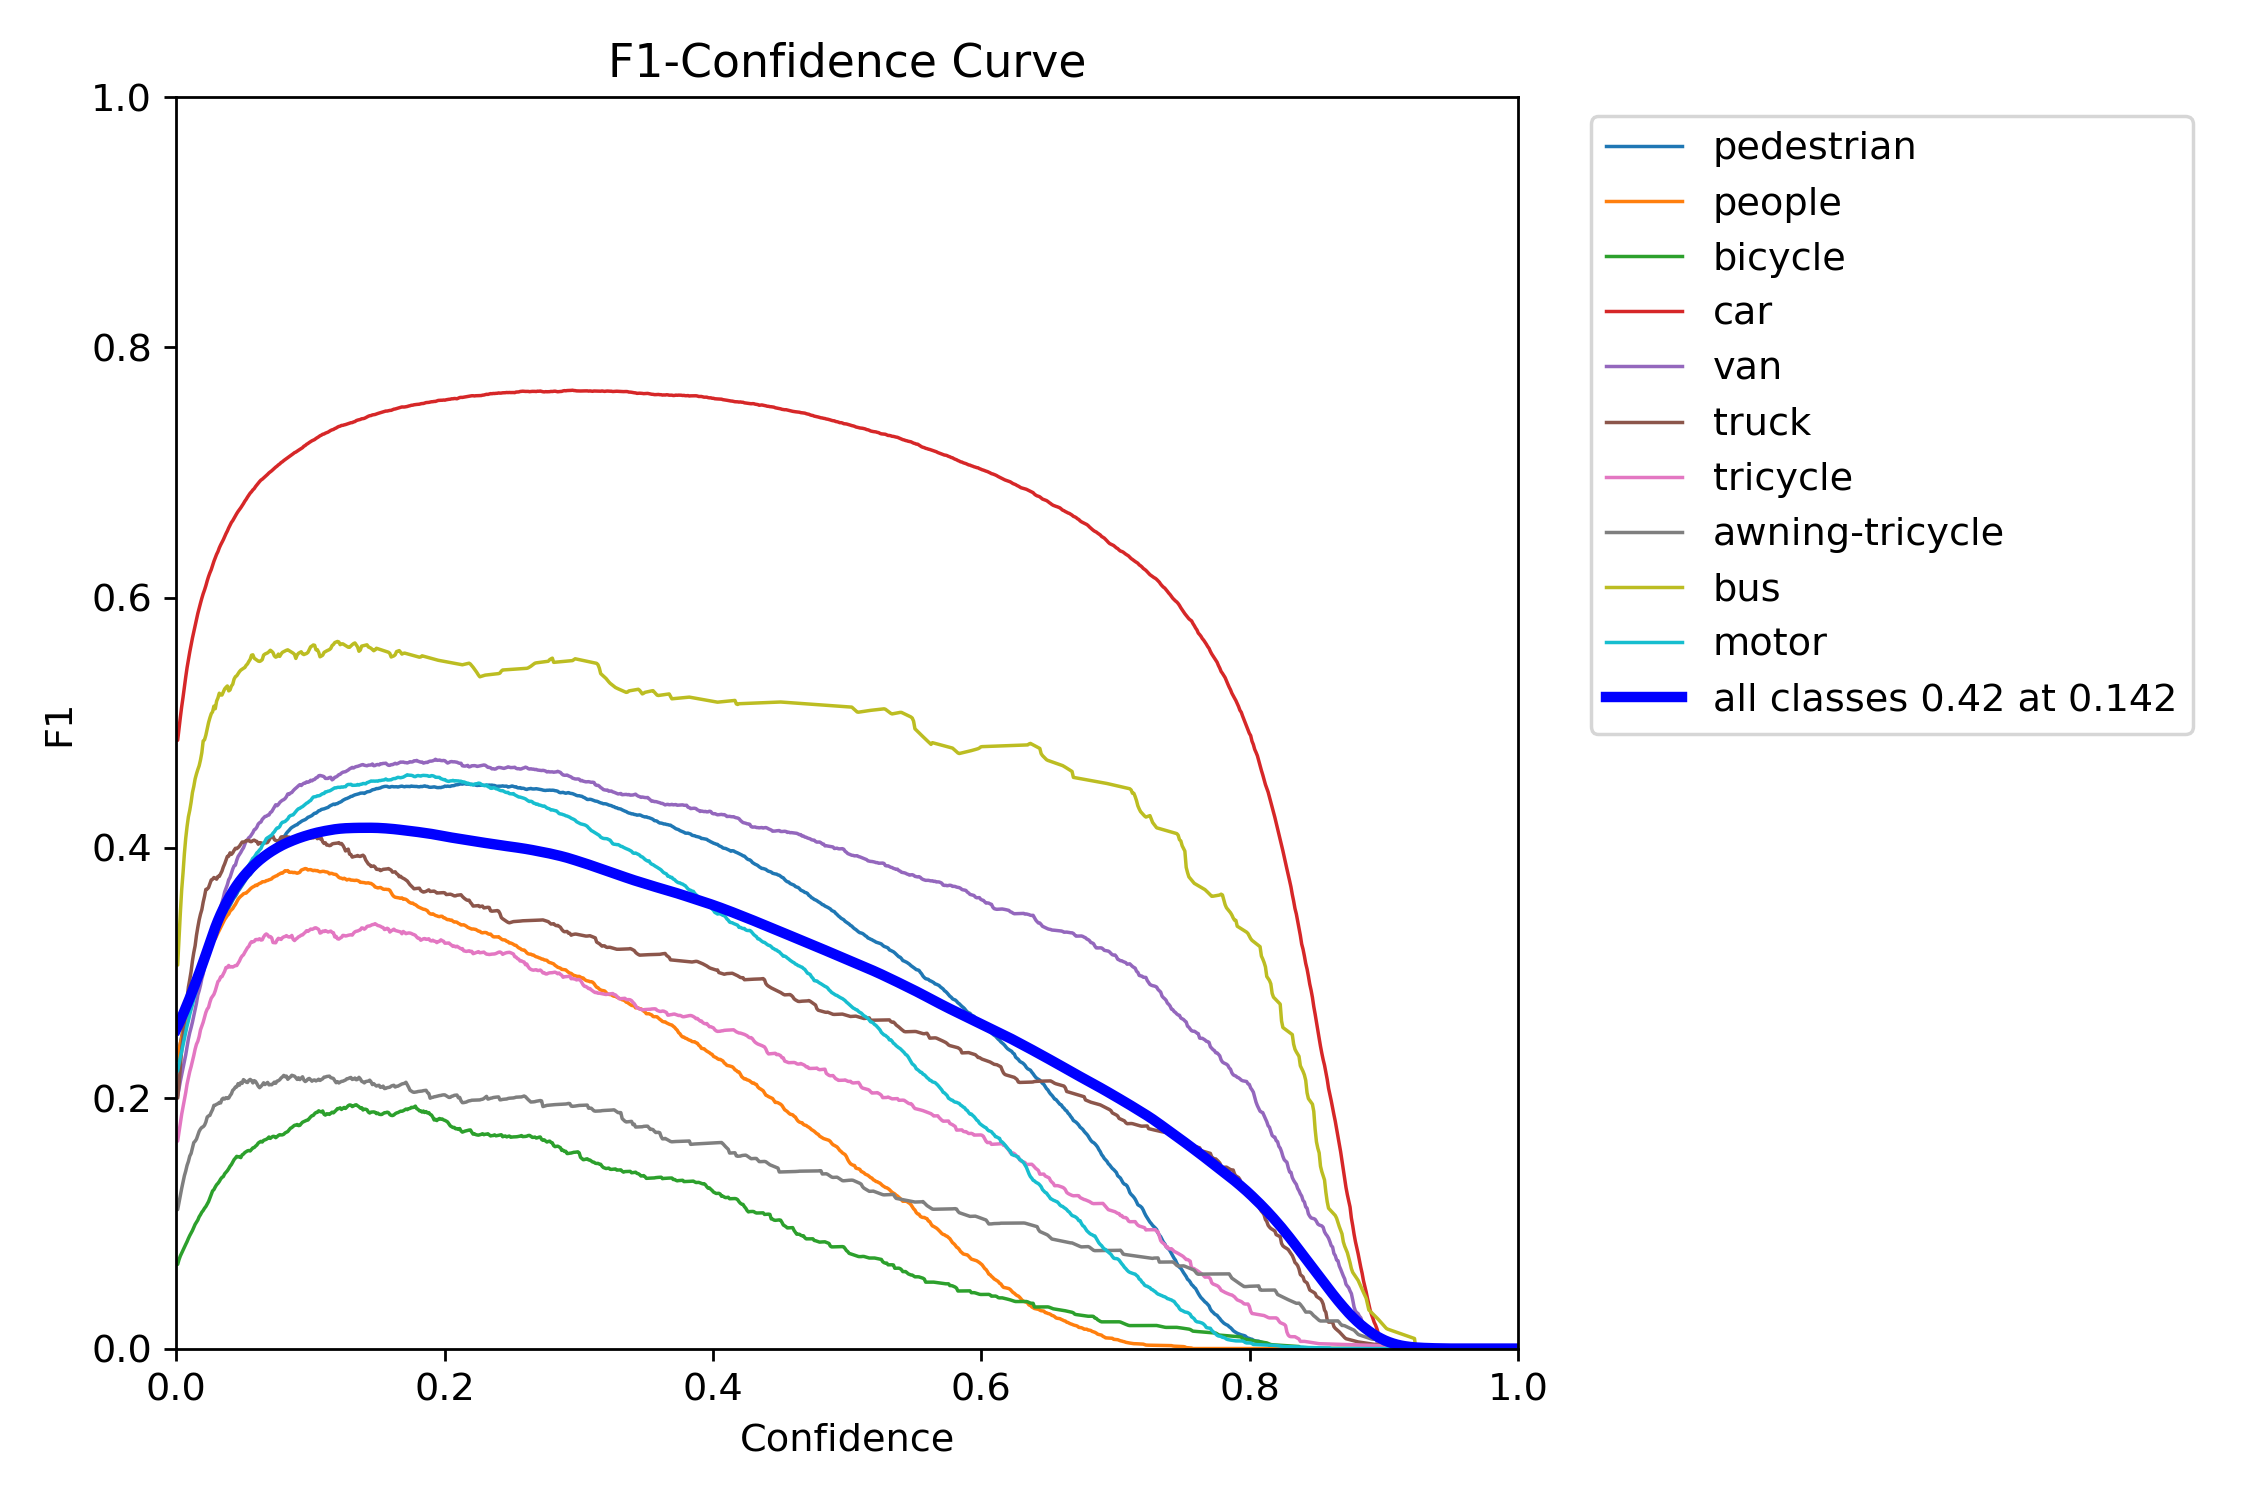
\includegraphics[width=0.4\textwidth]{../figure/vd_ex_F1_curve.png}
    }
    \subfloat[YOLOv11s\label{fig:vd_11s_f1}]{
        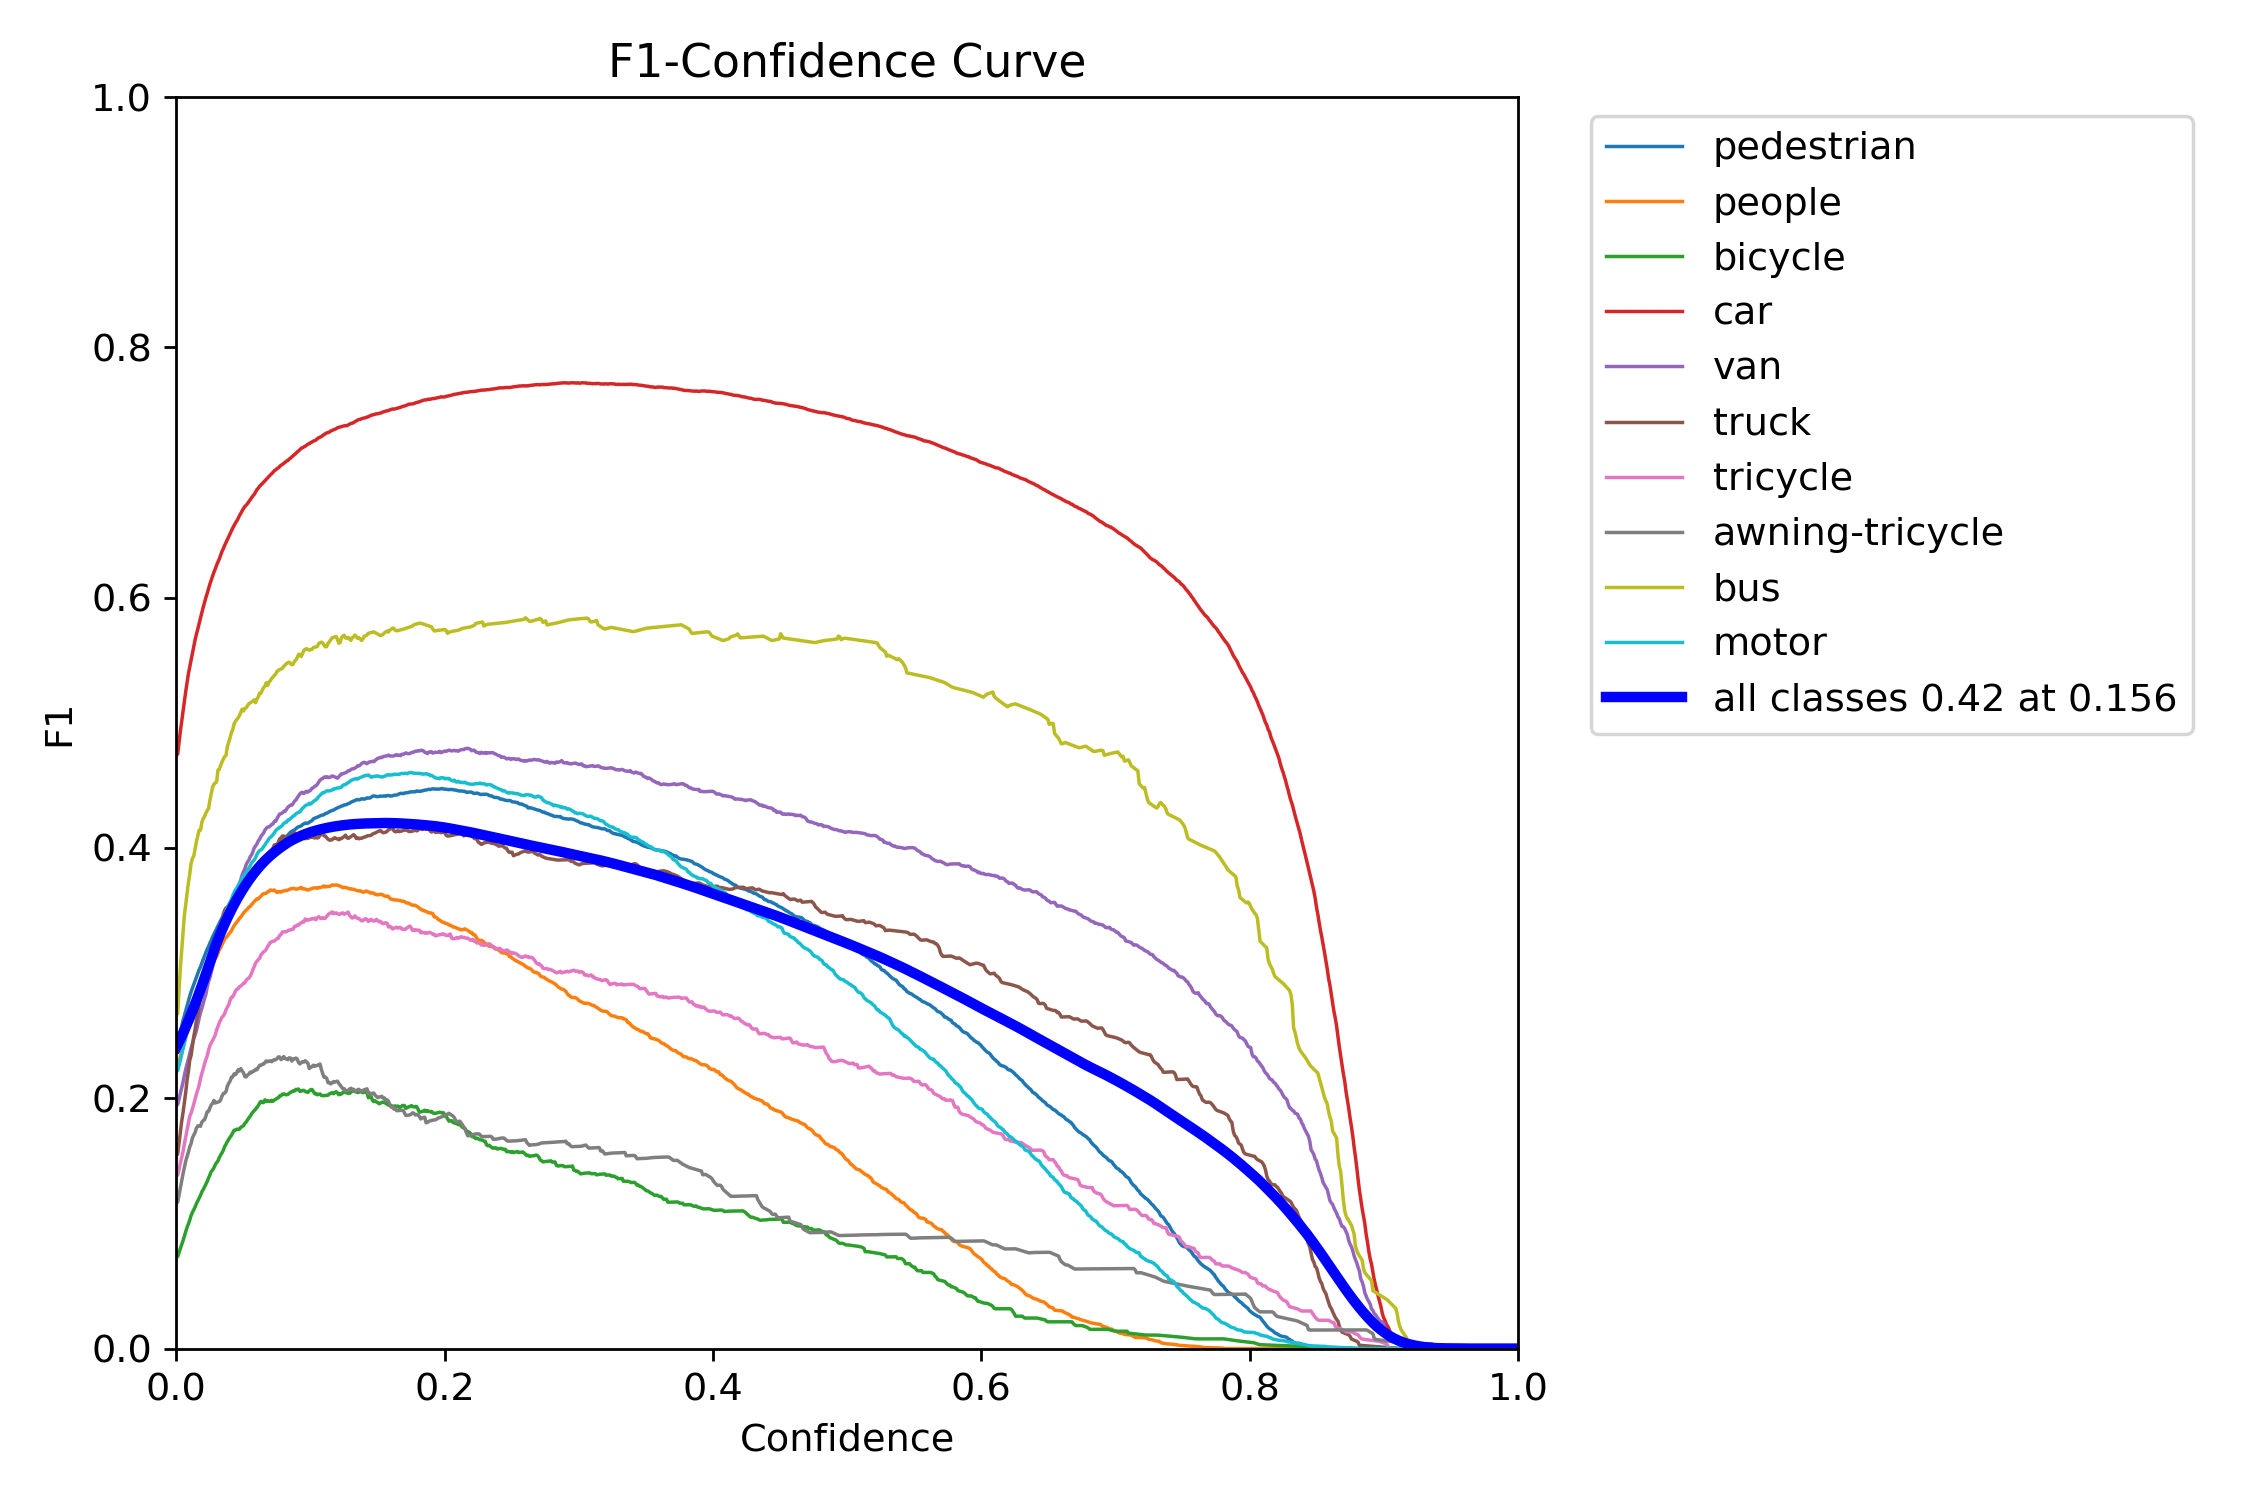
\includegraphics[width=0.4\textwidth]{../figure/vd_v11s_F1_curve.png}
    } \\
    \subfloat[YOLOv10s\label{fig:vd_10s_f1}]{
        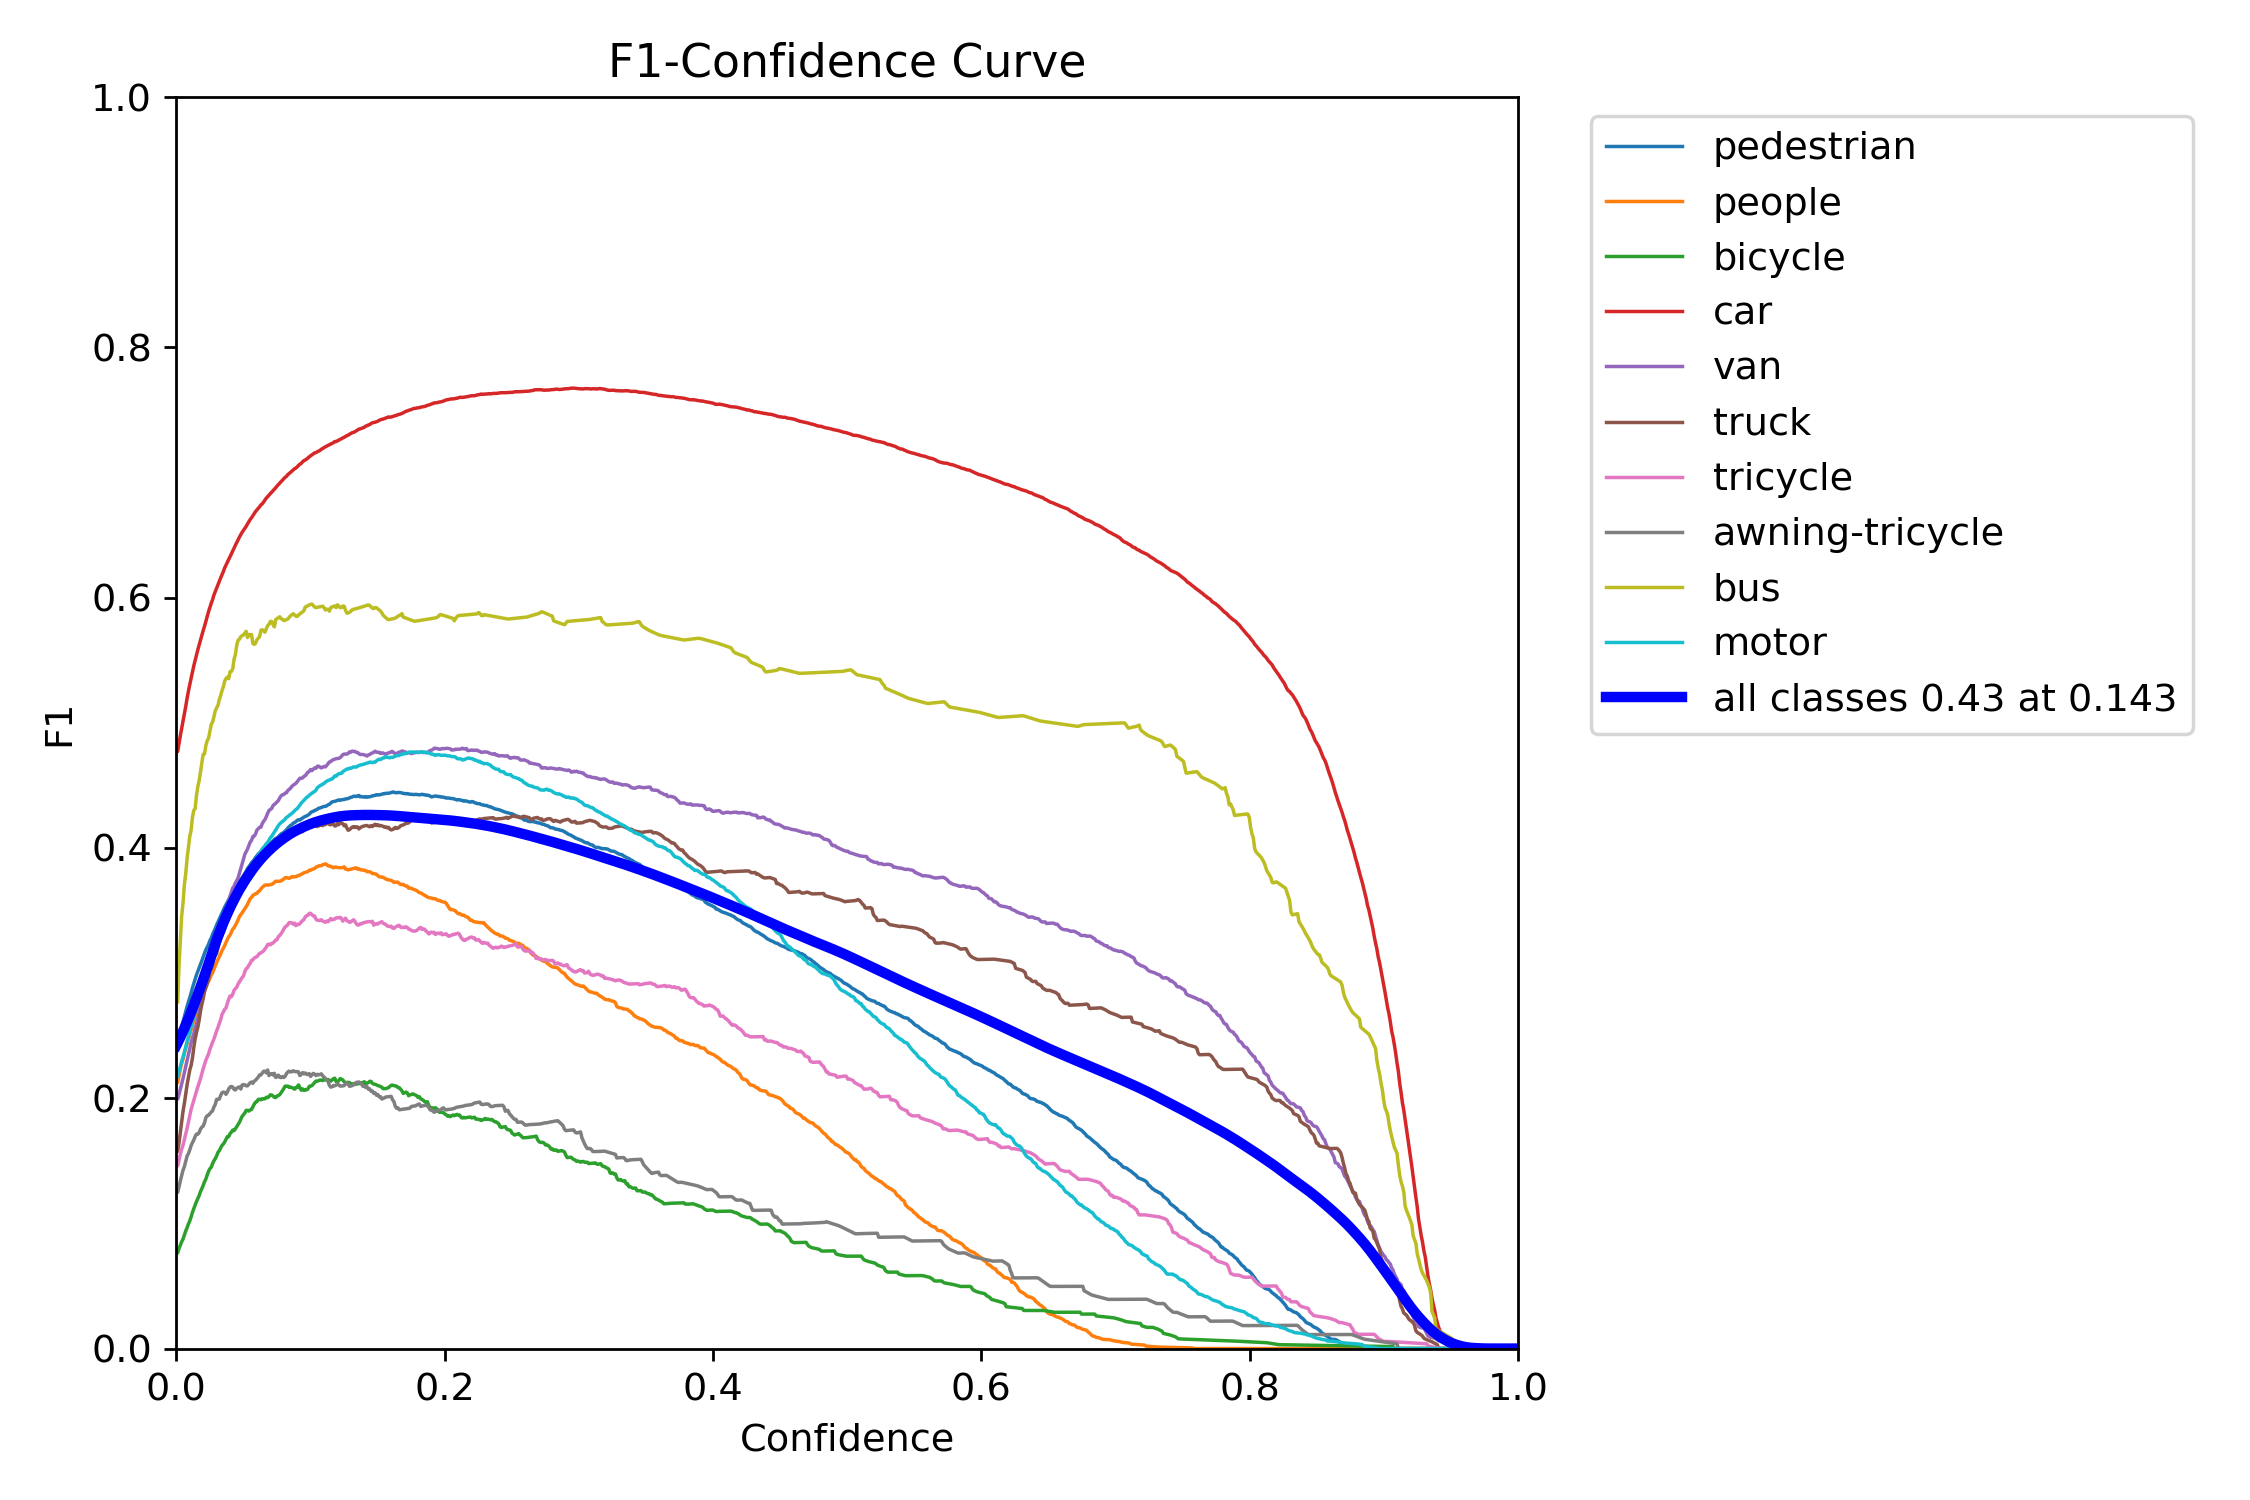
\includegraphics[width=0.4\textwidth]{../figure/vd_v10s_F1_curve.png}
    }
    \subfloat[YOLOv9s\label{fig:vd_9s_f1}]{
        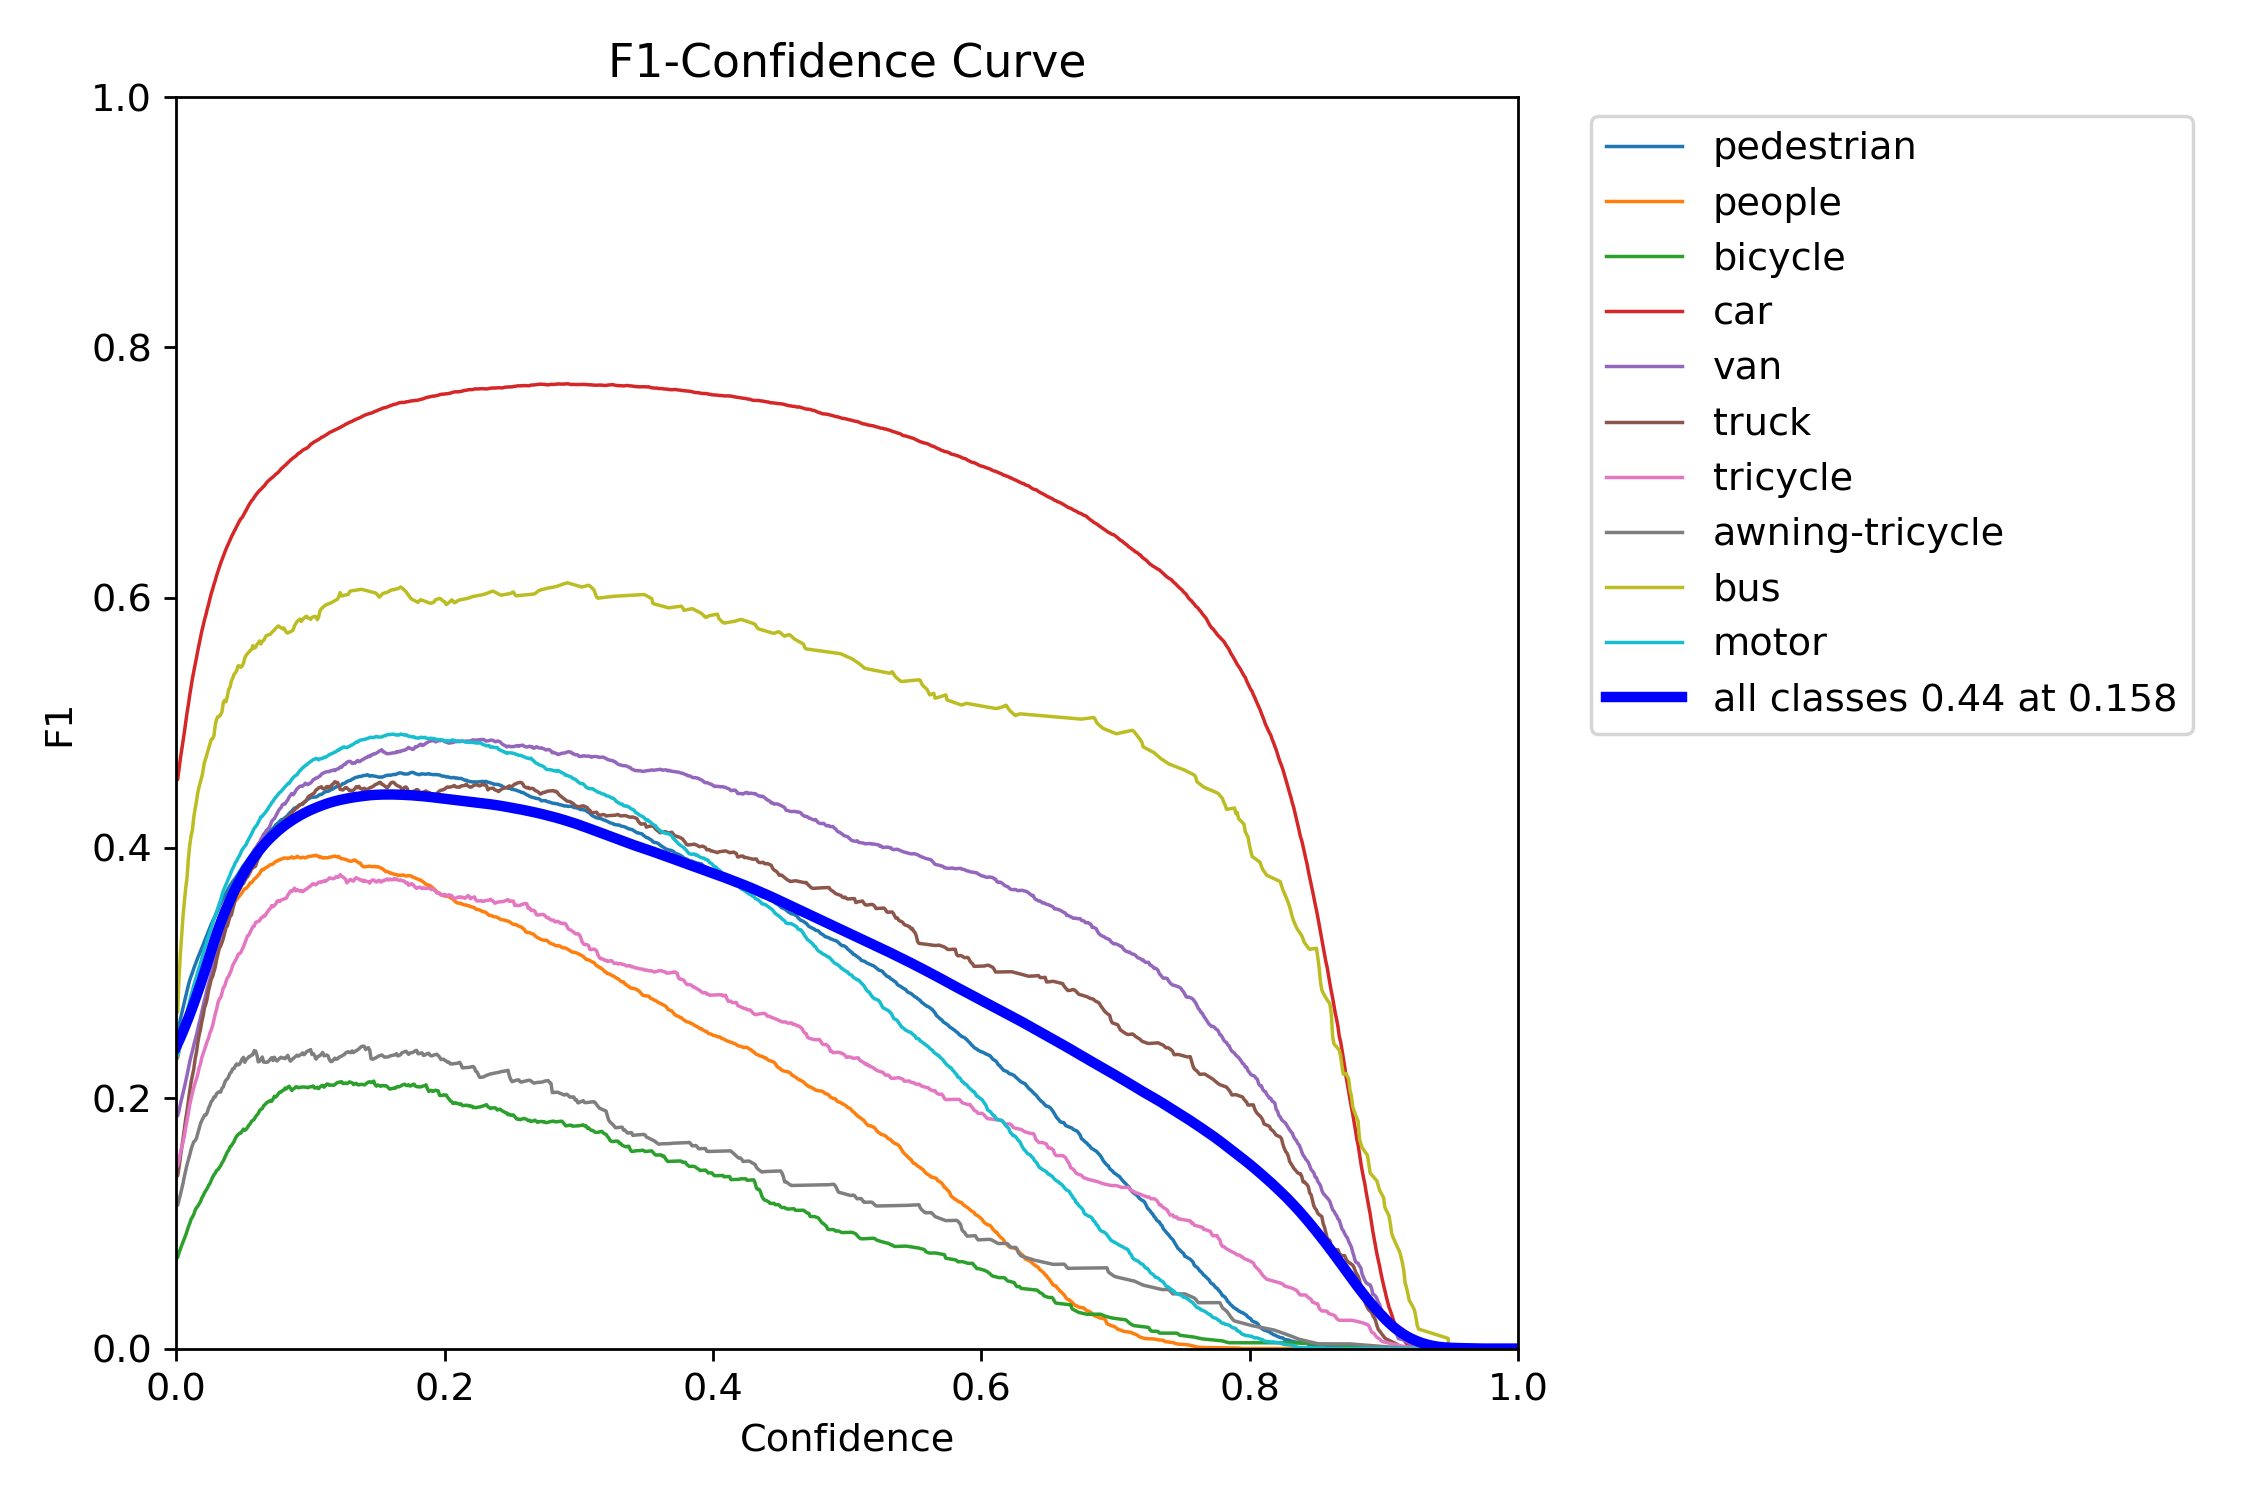
\includegraphics[width=0.4\textwidth]{../figure/vd_v9s_F1_curve.png}
    }
    \captionsetup{font=footnotesize}
    \bicaption{不同的网络模型在VidDrone数据集上的F1得分}{Symbol cross-reference table}
    \label{fig:vd_f1}
\end{figure}

在表 \ref{tab:compare_studies_vd} 中,就计算量(GFLOPs)而言,our 模型明显低于其他值为15.4的比较模型。 YOLOv11s是21.3,YOLOv10s是24.5,YOLOv9s高达26.7。 这一结果充分表明,改进后的算法在减少计算量方面取得了出色的效果。 较低的计算量有助于延长无人机的耐用性,并提高其在复杂环境中的运行效率,使其能够更快地处理图像数据并做出准确的判断。

在精度(P)方面,our 模型是0.514,高于YOLOv11s的0.485和YOLOv10s的0.501,略低于YOLOv9s的0.525。 在召回(R)方面,our 模型是0.372,略低于YOLOv11s的0.381和YOLOv10s的0.380,与YOLOv9的0.392相比存在一定的差距。

图 \ref{fig:vd_cmn} 展示了 YOLOv9s、YOLOv10s、YOLOv11s 以及 our 模型在 VisDrone 数据集针对不同类别目标的预测状况,以归一化混淆矩阵热力图形式呈现。热力图颜色深浅与预测概率正相关,颜色愈深表示预测准确率愈高,颜色愈浅则表明预测准确率较低。对角线数据反映模型成功预测正确标签的情况,非对角线数据则体现模型标签预测错误的情形。

从图 \ref{fig:vd_ex_cmn} 至图 \ref{fig:vd_9s_cmn} 可见,各模型在不同类别上的预测表现存在差异。
综合归一化混淆矩阵热力图信息可知,在 VisDrone 数据集上,YOLOv9s 模型在预测正确类别方面表现较为出色,这一结论与表 \ref{tab:compare_studies_vd} 中的数据相呼应 —— YOLOv9s 的精确度(0.525)和召回率(0.392)均处于较高水平。our 模型的精确度(0.514)略低于 YOLOv9s,但召回率(0.372)与 YOLOv11s(召回率 0.381)和 YOLOv10s(召回率 0.380)相近,整体性能优于 YOLOv10s 模型。尽管 our 模型在精确度和召回率上未超越 YOLOv9s,但其在特定类别预测上展现出独特优势,例如在 “pedestrian” 和 “awning-tricycle”类别预测中,our 模型的准确率达到了 0.35 和 0.13,相较于其他模型具有一定的竞争力。
总体而言,our 模型在 VisDrone 数据集上的表现与 YOLO 系列模型各有优劣。虽然在精确度和召回率上略逊于 YOLOv9s,但在部分类别预测上展现出独特优势,且整体性能优于 YOLOv10s 模型,与 YOLOv11s 模型相近,具有进一步优化和提升的潜力。

从$mAP_{0.5}$的主要性能指数来看,our 模型达到了0.390,与YOLOv10s相同,高于YOLOv11s的0.383,略低于YOLOv9s的0.402。 虽然YOLOv9s的mAP最高,但其计算量也是最大的,这在一定程度上限制了其在实际应用中的可行性。 相比之下,our 模型仍然保持高mAP,同时有效减少计算量,这反映了改进算法在提高检测精度方面的优势。 在无人机的小目标检测任务中,关键是准确识别各种目标。 our 模型可以在复杂的场景中更好地完成这项任务,这对于提高无人驾驶飞行器在实际应用中的可靠性和有效性具有重要意义。

至于FPS,FPS受到硬件的极大影响。 我们的型号是68.5,低于YOLOv11的82.6和YOLOv10的78.1,但高于YOLOv9的62.1。 our 模型可以实现相对可观的FPS,同时保持低计算量和高mAP,这表明它在处理速度方面也具有竞争力。

从mAP的角度来看,YOLOv9s的mAP是最高的(0.402),这与其较高的F1 AUC一致。 我们模型的mAP是0.390,与YOLOv10s相同,但F1 AUC略低。 这表明,尽管our 模型在平均精度上与YOLOv10s相当,但不同F1分数水平的综合性能不如YOLOv10s稳定。 F1曲线的差异可能反映了我们模型在某些F1分数区间中的性能波动。

通过对TT100K和VisDrone数据集的全面测试,我们改进的模型在小目标检测领域显示出竞争优势,特别是在资源有限的应用场景中。 我们的实验验证了SPPC模块、DBSS模块和NWD损失函数组合在提高检测性能和优化计算效率方面的贡献。 总的来说,这些改进增强了YOLOv11模型在小目标检测任务中的实用性,减少了对计算资源的需求,并使其更适合无人机等有限设备环境中的实际应用。

接下来使用消融实验分析不同改进方法对模型的影响。经过多次实验,根据硬件设施和多次实验尝试,我们设置了以下参数:BatchSize = 8,Epoch=300。 为了清楚地显示实验的真实性,本实验采用平均精度$mAP_{0.5}$作为性能评估指数,计算量(GFLOPs)作为计算量评估指数,参数量、精度率和召回率作为参考指标。 测试结果显示在表\ref{tab:ablation_studies_tt100k}和\ref{tab:ablation_studies_vd}中。 下表显示了每个模型的性能指标,包括平均精度($mAP_{0.5}$)、参数体积、计算量(GFLOPs)、精度率、召回率和FPS。

\begin{table*}[htbp]
    \centering
    \captionsetup{font=footnotesize}
    \bicaption{在TT100K数据集上的消融实验}{Symbol cross-reference table}
    \label{tab:ablation_studies_tt100k}
    \begin{tabular}{p{0.22\textwidth}p{0.1\textwidth}p{0.12\textwidth}p{0.07\textwidth}p{0.07\textwidth}p{0.07\textwidth}p{0.07\textwidth}}
        \toprule
        模型       & 参数量 MB & 计算量 GFLOPs & $mAP_{0.5}$   & P     & R     & FPS \\ 
        \midrule
        YOLOv11s(base) & 9.5           & 21.8         & 0.877          & 0.878  & 0.777 & 94.3 \\
        +NWD           & 9.5           & 21.8         & 0.882          & 0.876  & 0.802 & 95.2 \\
        +NWD+SPPC      & 11.5          & 26.5         & \textbf{0.909} & 0.877  & 0.827 & 78.1 \\
        +NWD+SPPC+DBSS & 11.4          & \textbf{17.0} & 0.893          & 0.875  & 0.830 & 84.7 \\
        \bottomrule
    \end{tabular}
\end{table*}

\begin{table*}[htbp]
    \centering
    \captionsetup{font=footnotesize}
    \bicaption{在VisDrone数据集上的消融实验}{Symbol cross-reference table}
    \label{tab:ablation_studies_vd}
    \begin{tabular}{p{0.22\textwidth}p{0.1\textwidth}p{0.12\textwidth}p{0.07\textwidth}p{0.07\textwidth}p{0.07\textwidth}p{0.07\textwidth}}
        \toprule
        模型       & 参数量 MB & 计算量 GFLOPs & $mAP_{0.5}$   & P     & R     & FPS \\ 
        \midrule
        YOLOv11s(base) & 9.4           & 21.3          & 0.383          & 0.485  & 0.381 & 82.6 \\
        +NWD           & 9.4           & 21.3          & 0.386          & 0.498  & 0.382 & 80.0 \\
        +NWD+SPPC      & 11.4          & 26.0          & \textbf{0.392} & 0.527  & 0.367 & 63.7 \\
        +NWD+SPPC+DBSS & 11.4          & \textbf{15.4} & 0.390 & 0.514  & 0.372 & 68.5 \\
        \bottomrule
    \end{tabular}
\end{table*}

在表 \ref{tab:ablation_studies_tt100k} 中,在TT100K数据集中,引入基于YOLOv11s(base)的NWD损失函数后,$mAP_{0.5}$从0.877增加到0.882,增加了0.5\%,召回率从0.777增加到0.802,精度略有下降。 计算和参数保持不变,FPS略有改进,表明NWD损失函数提高了识别小目标的能力,对计算效率影响不大。 然后添加SPPC模块,$mAP_{0.5}$跃升到0.909,增加3.6\%,精度稳定,召回率达到0.827,但参数增加到11.5MB,计算量上升到26.5GFLOPs,增加21\%,FPS下降,表明性能有所提高,对计算资源的需求增加。 但在高精度检测的情况下,这是合理的。 最后,添加了DBSS模块,计算量减少到17.0GFLOPs,减少了22\%,$mAP_{0.5}$略微减少到0.893,增加了1.8\%。 精度和召回率保持在高水平,FPS反弹,表明DBSS模块在保持检测性能的同时减少了计算量,并实现了效率。 利率的平衡。

在表 \ref{tab:ablation_studies_vd} 中,在VisDrone数据集中,以YOLOv11s(base)为起点,在引入NWD损失函数后,$mAP_{0.5}$从0.383增加到0.386,增加了0.7\%,精度从0.485增加到0.498,召回率保持不变。 计算量和参数保持不变,FPS略低,这对计算效率影响不大。 添加SPPC模块后,$mAP_{0.5}$达到0.392,增加2.4\%,精度提高到0.527,召回率降低但检测性能提高,参数增加到11.4MB,计算量增加到26.0GFLOPs,增加22\%,FPS显著下降,提高检测性能但增加计算资源要求。 最后,引入了DBSS模块,计算量减少到15.4GFLOPs,减少了27\%,$mAP_{0.5}$略微减少到0.390,但仍比基础高出2\%。 精度和召回率保持在良好的水平,FPS反弹,表明DBSS模块有效地减少了计算量,同时保持了检测性能并改进了模块。 复杂场景下的运营效率和适应性。

基于表 \ref{tab:ablation_studies_tt100k} 和表 \ref{tab:ablation_studies_vd} 的i消融实验结果,NWD损失函数在一定程度上提高了模型对小目标的检测性能,特别是在提高召回率方面,这在无人机小目标的检测任务中发挥了积极作用;SPPC该模块显著增强了模型的特征提取和识别能力,大大提高了$mAP_{0.5}$,但也增加了模型的计算量和参数规模;DBSS模块在减少模型计算量方面取得了显著效果,可以在保持高检测性能的同时减少计算资源的消耗。 消耗和提高模型的运行效率对于平衡无人驾驶飞行器在实际应用中的检测精度和计算效率具有关键意义。 通过这些减值实验,我们在不同数据集和小目标检测场景下验证了拟议改进模块的有效性,这为改进YOLOv11算法以增强无人机的小目标检测性能提供了强有力的支持和重要参考。

为了直观地看到EX-YOLO的检测效果,选择了两组复杂的场景图进行测试。 使用EX-YOLO、YOLOv11s、YOLOv10s和YOLOv9s的加权文件被保留并用于测试和比较。 图像选择标准包括具有不同尺寸和重叠目标的复杂场景。 基于上述要求,可以清楚地看到EX-YOLO、YOLOv11s、YOLOv10s和YOLOv9s之间的差异。 其中,图\ref{fig:tt100k_compare_1}和图\ref{fig:tt100k_compare_2}显示了与密集小目标分布在图片边缘的复杂场景的比较,图\ref{fig:vd_compare_1}和图\ref{fig:vd_compare_2}显示了与密集小目标和不同类别的复杂场景的比较。

\begin{figure}[htbp]
    \centering
        \subfloat[EX-YOLO\label{fig:tt100k_1_ex}]{%
            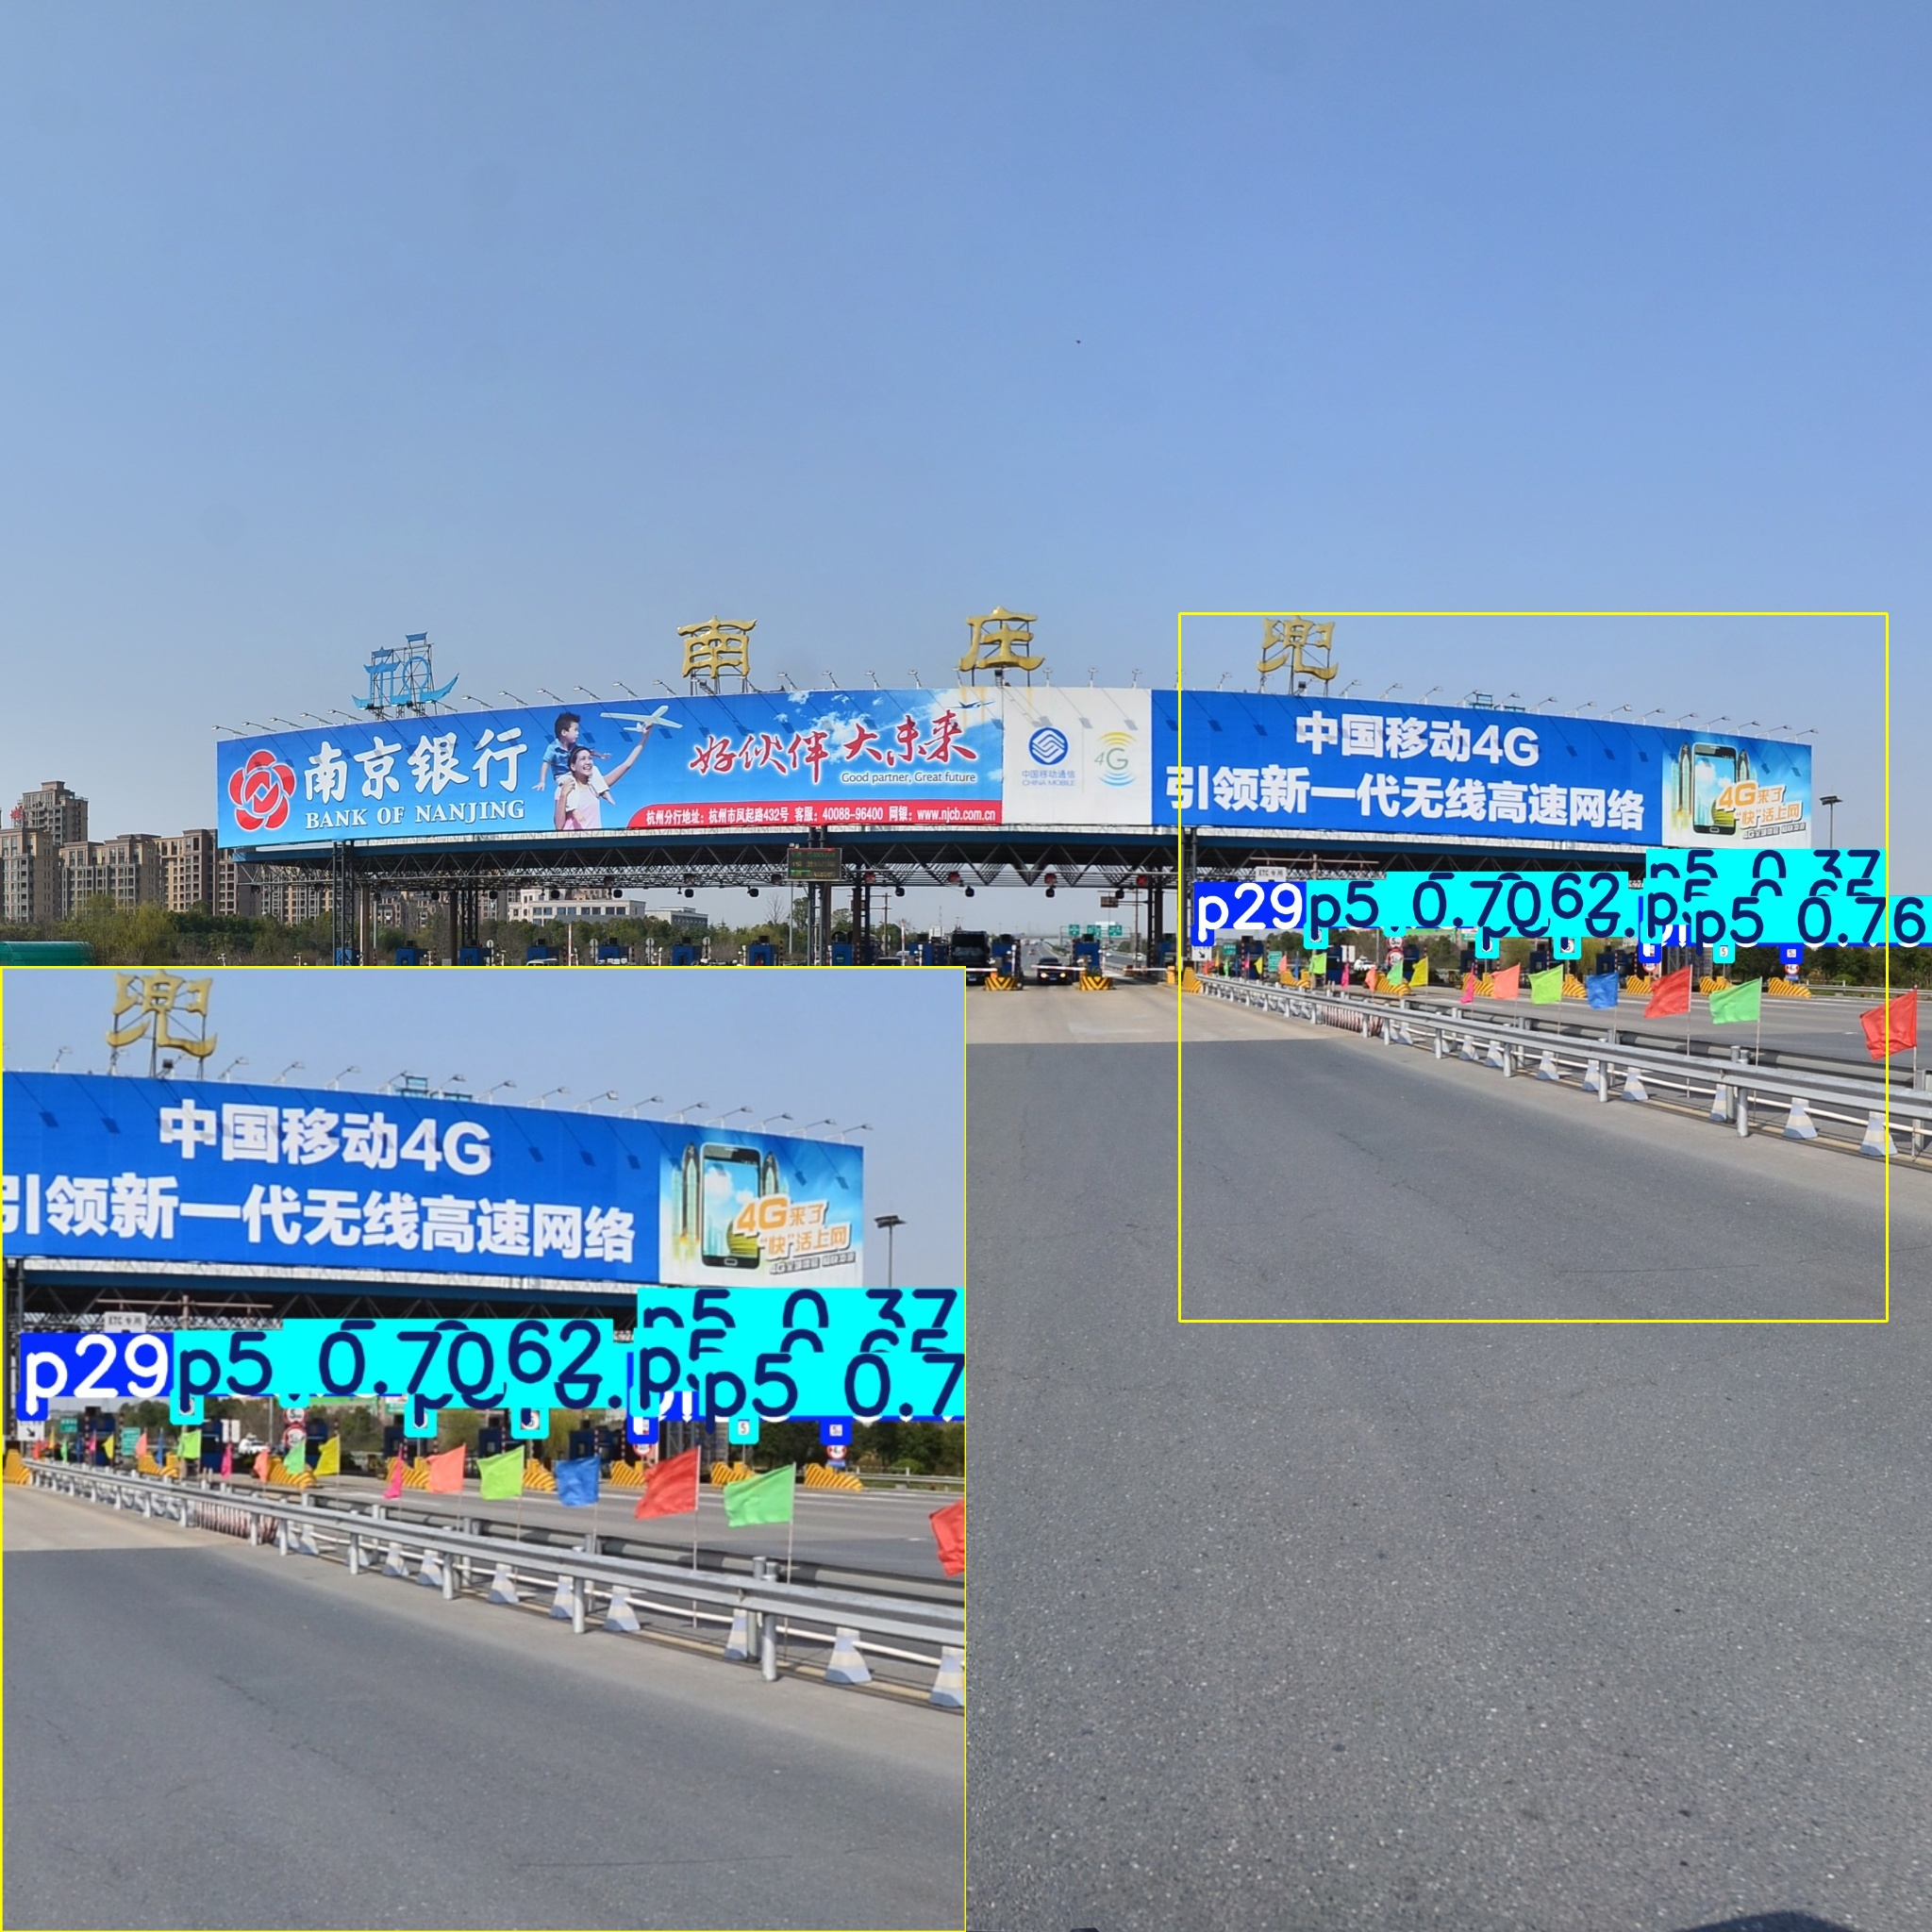
\includegraphics[width=0.33\textwidth]{../figure/ex-yolos_tt100k_44171.jpg}%
        } 
        \subfloat[YOLOv11s\label{fig:tt100k_1_11}]{%
            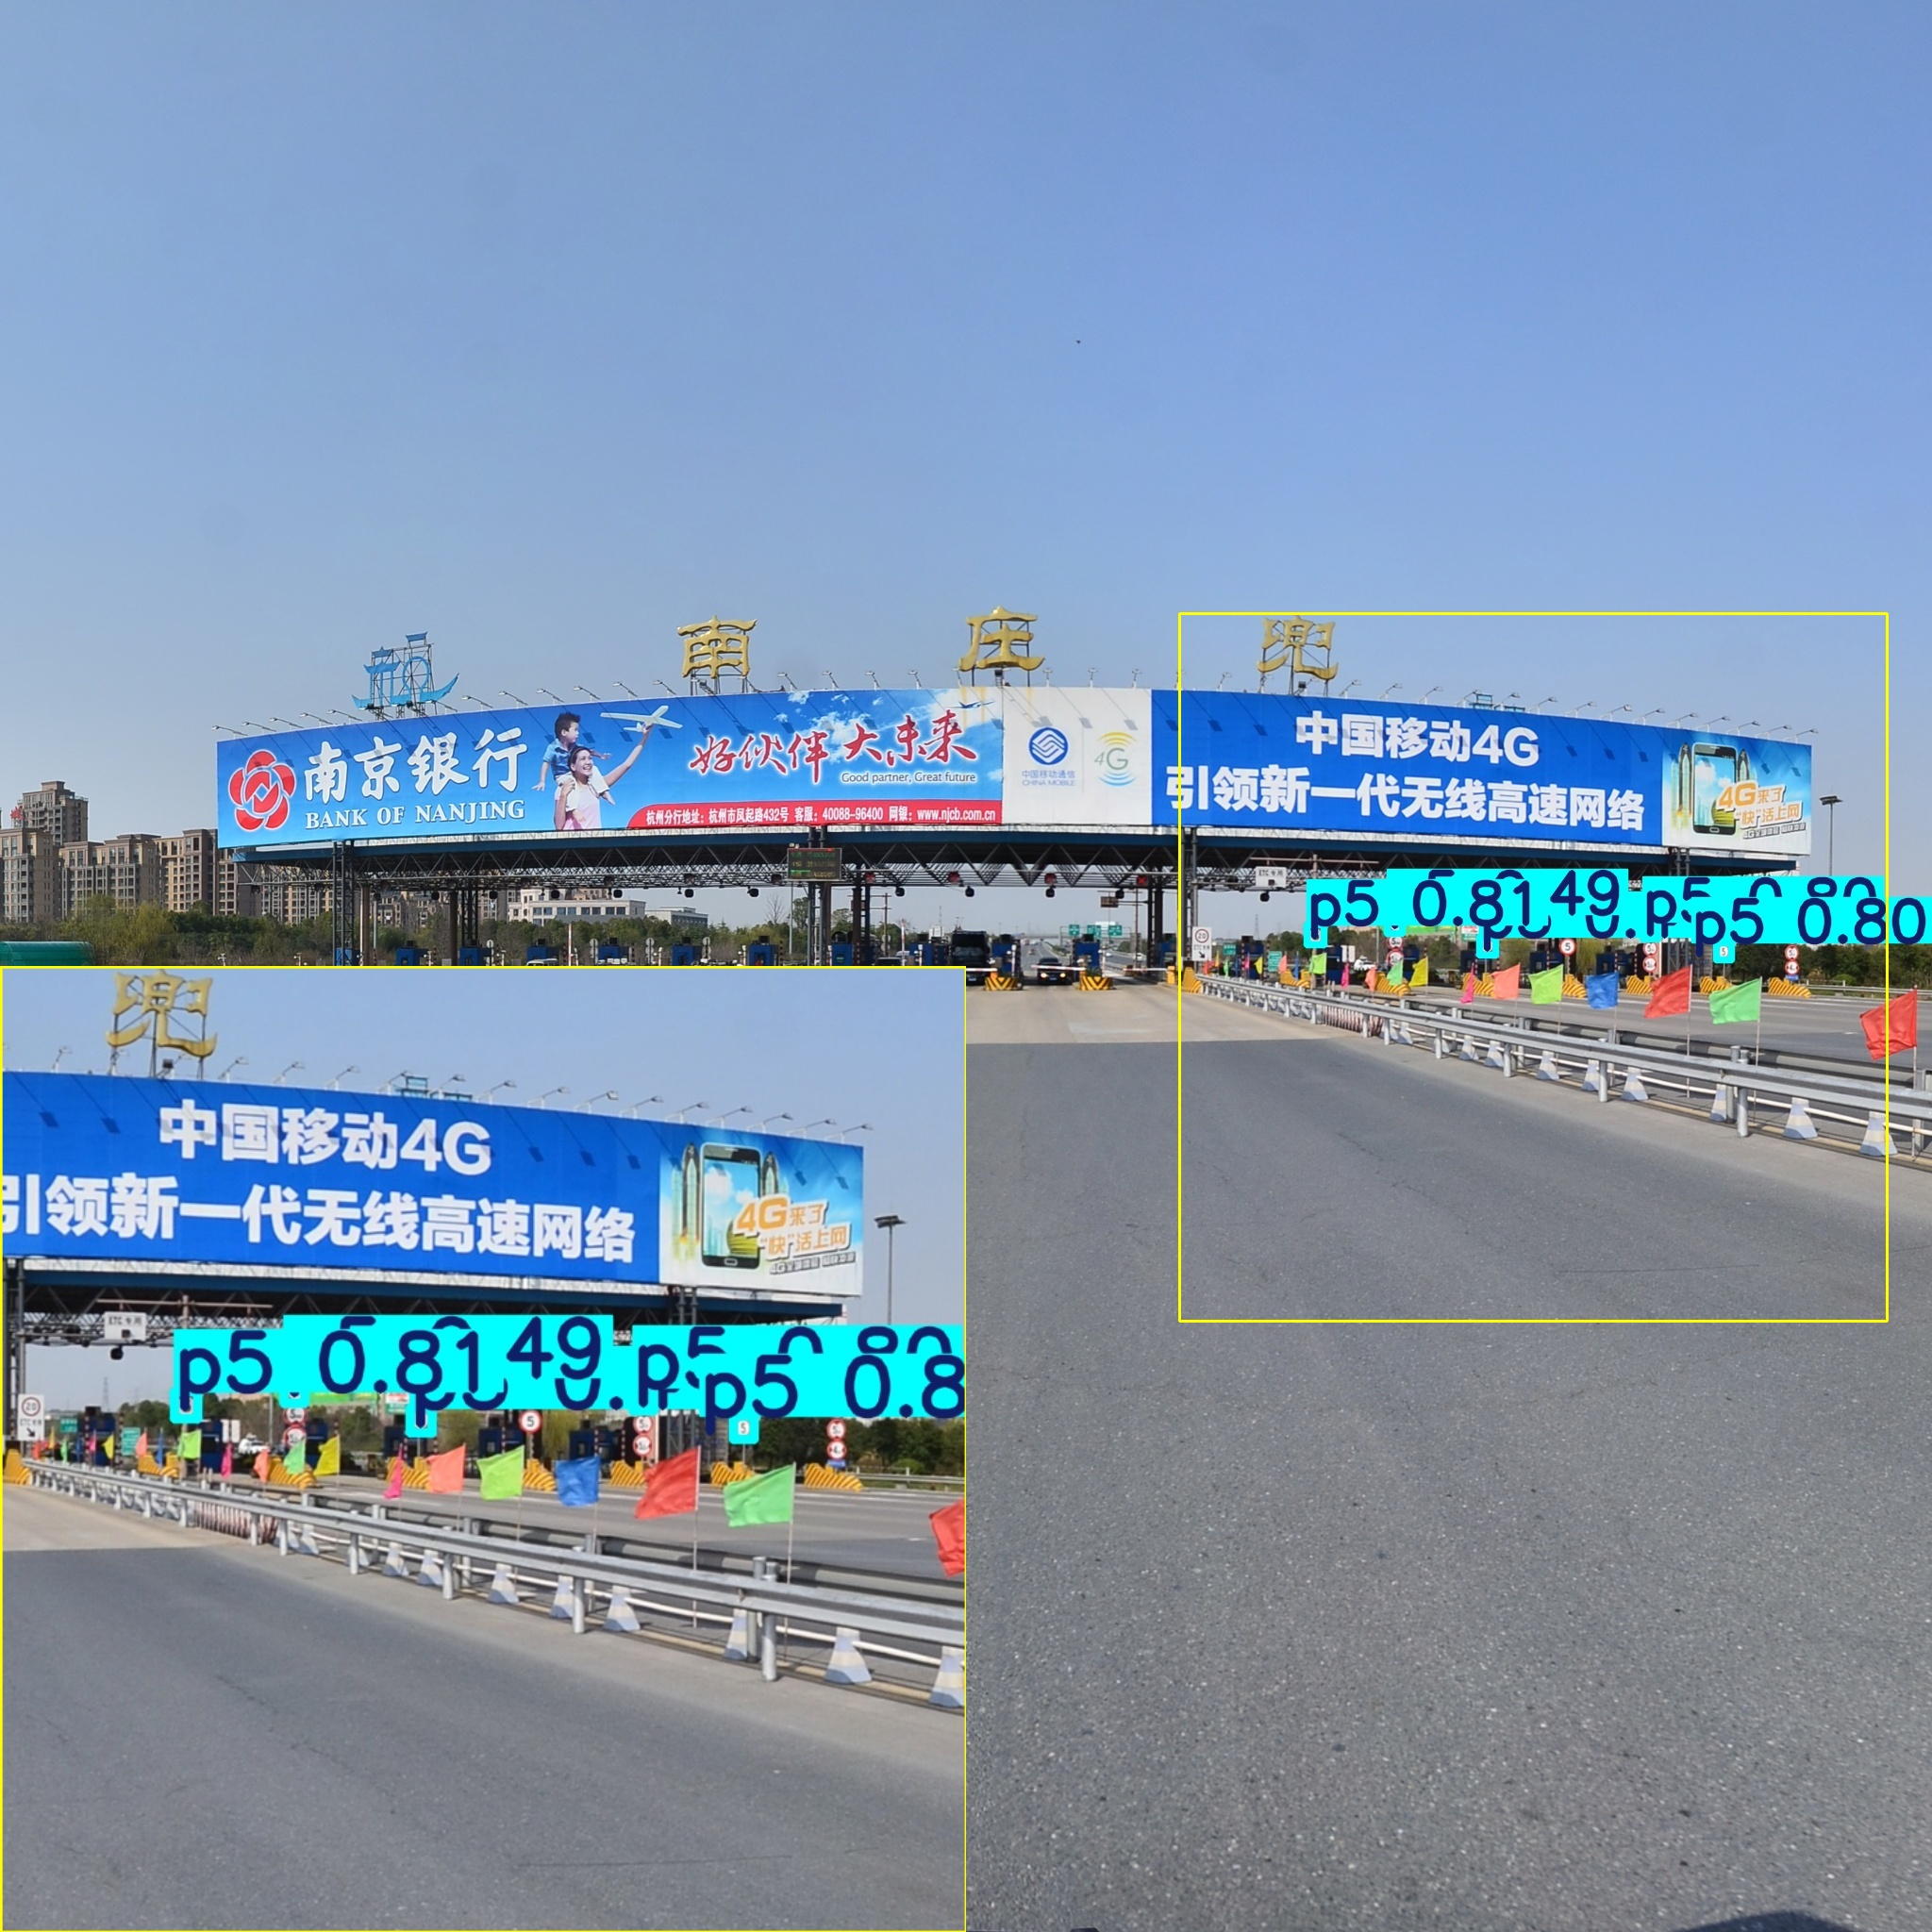
\includegraphics[width=0.33\textwidth]{../figure/v11s_tt100k_44171.jpg}%
        }
        \\
        \subfloat[YOLOv10s\label{fig:tt100k_1_10}]{%
            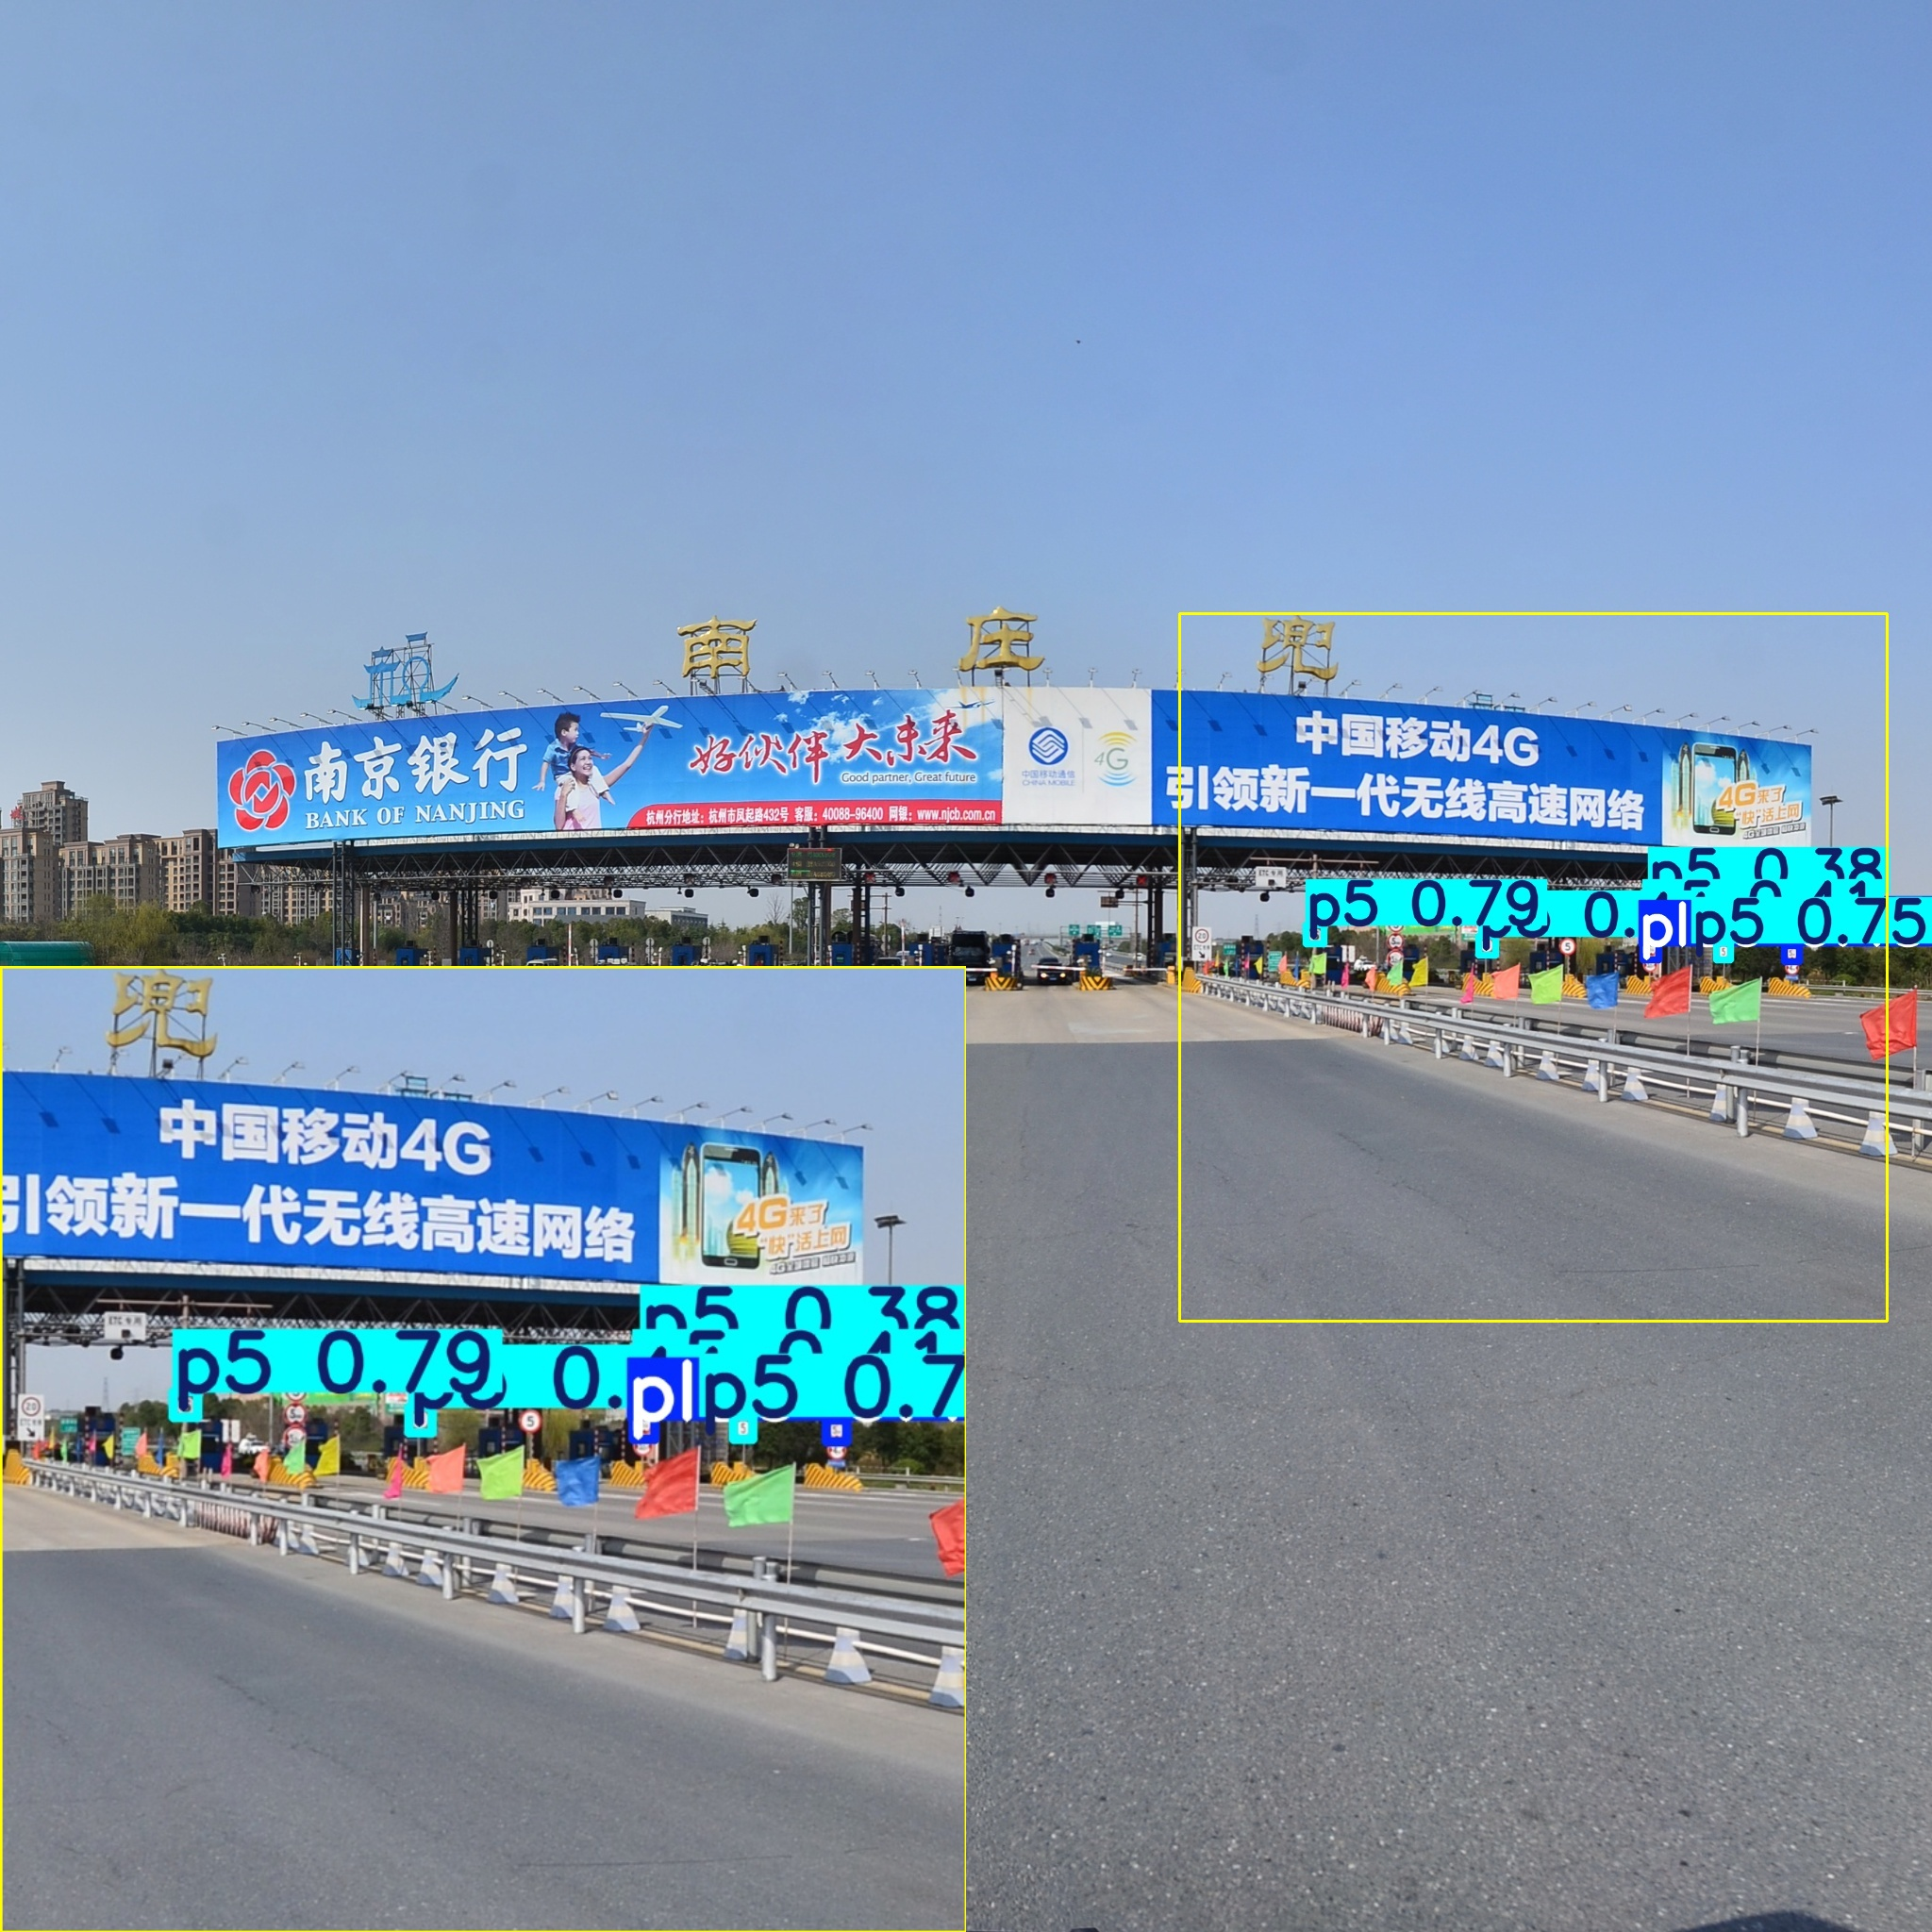
\includegraphics[width=0.33\textwidth]{../figure/v10s_tt100k_44171.jpg}%
        }
        \subfloat[YOLOv9s\label{fig:tt100k_1_9}]{%
            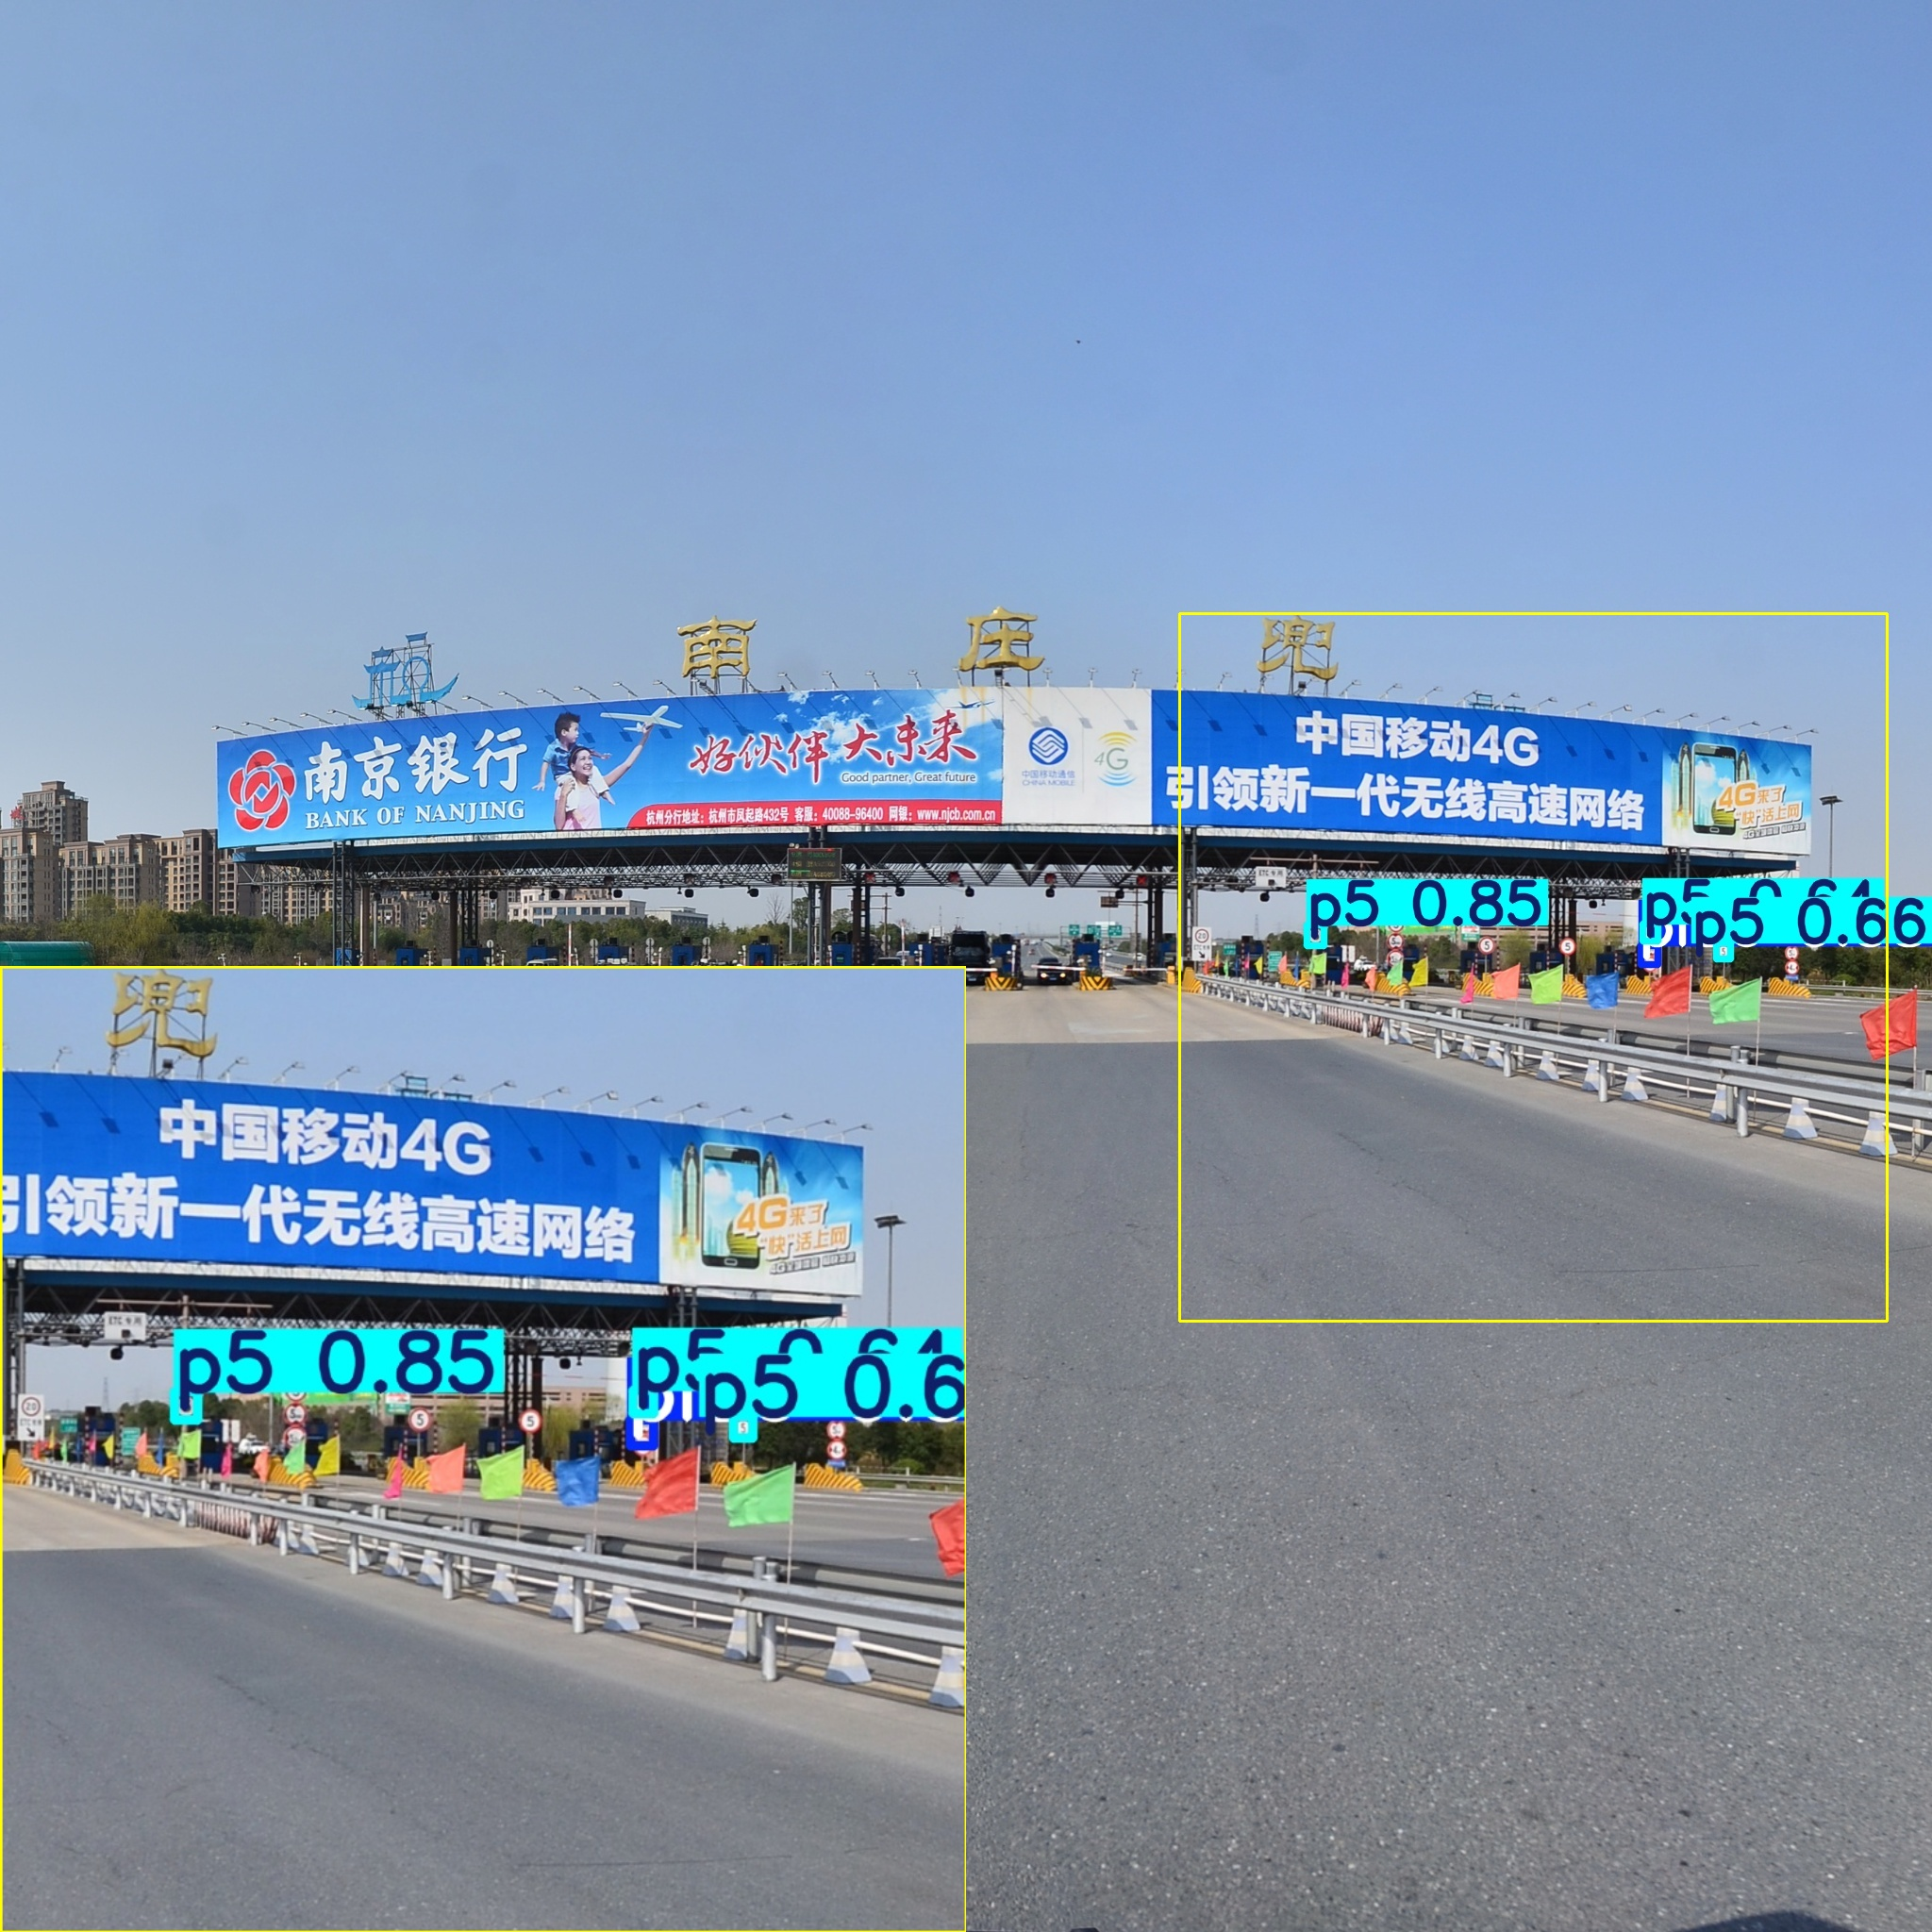
\includegraphics[width=0.33\textwidth]{../figure/v9s_tt100k_44171.jpg}%
        }
    \captionsetup{font=footnotesize}
    \bicaption{不同网络模型在TT100K数据集上的推理结果}{Some descriptions of the pictures in question.}
    \label{fig:tt100k_compare_1}
\end{figure}

\begin{figure}[htbp]
    \centering
        \subfloat[EX-YOLO\label{fig:tt100k_2_ex}]{%
            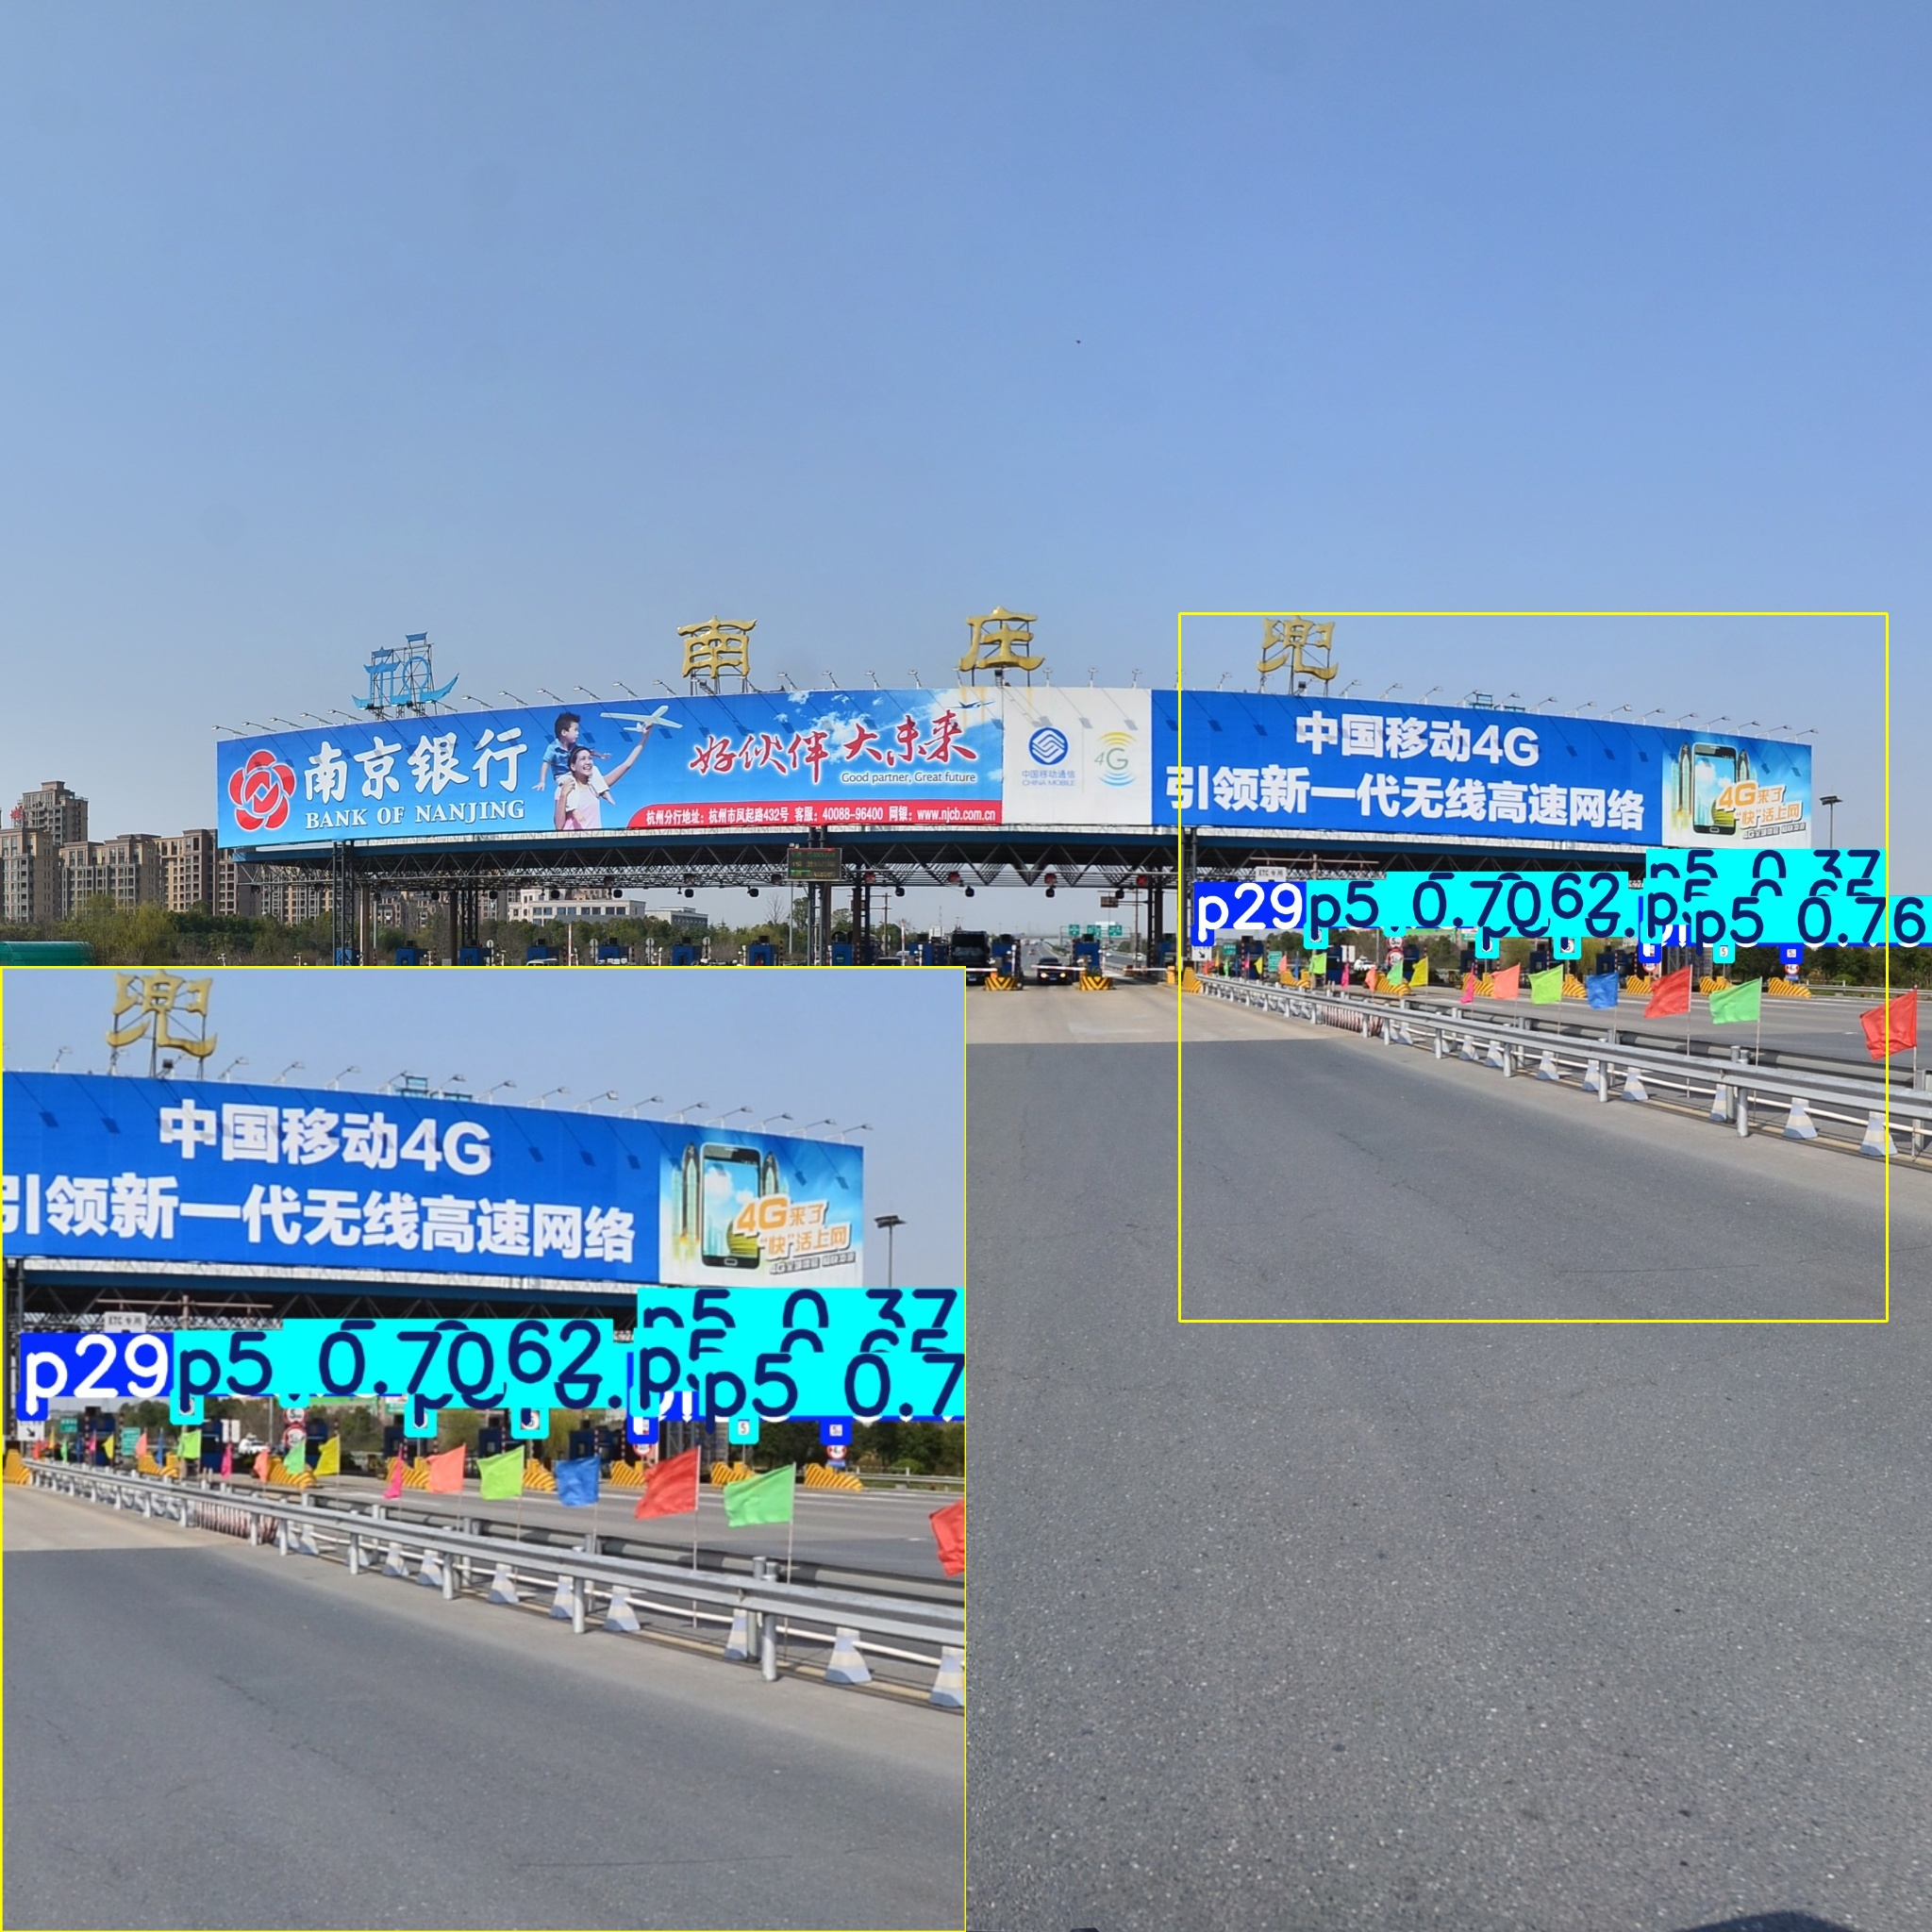
\includegraphics[width=0.33\textwidth]{../figure/ex-yolos_tt100k_44171.jpg}%
        } 
        \subfloat[YOLOv11s\label{fig:tt100k_2_11}]{%
            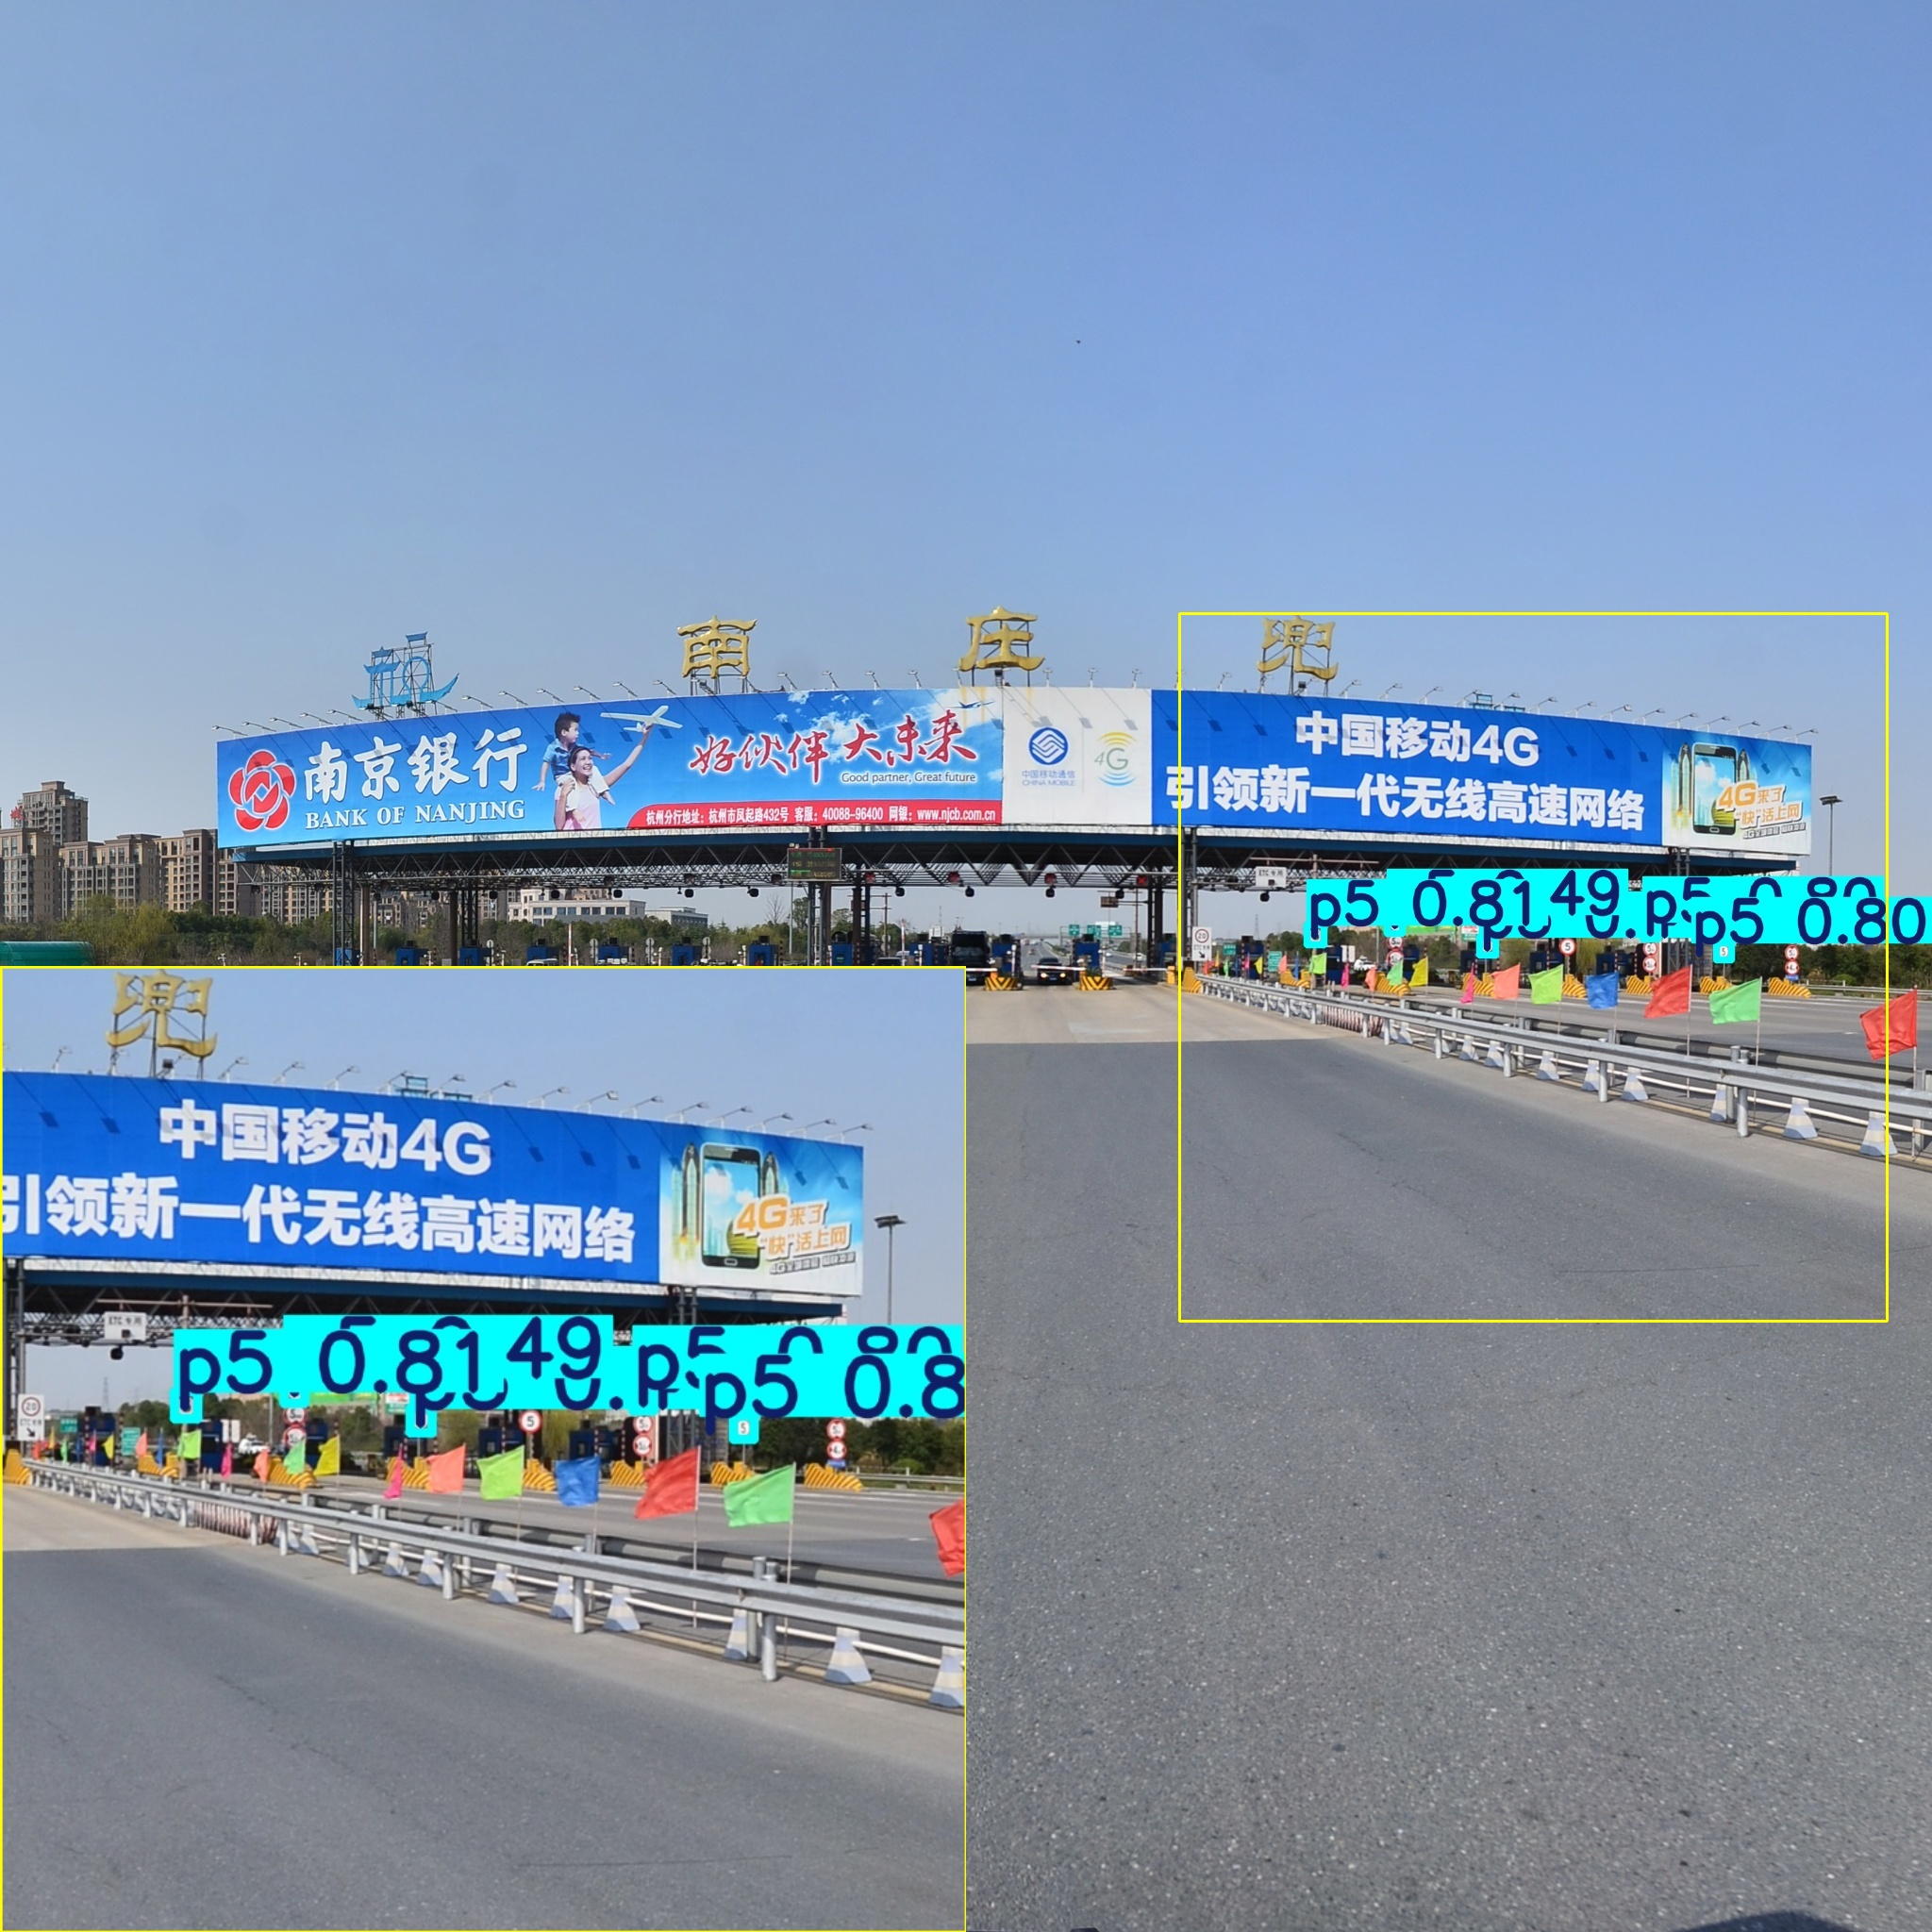
\includegraphics[width=0.33\textwidth]{../figure/v11s_tt100k_44171.jpg}%
        }
        \\
        \subfloat[YOLOv10s\label{fig:tt100k_2_10}]{%
            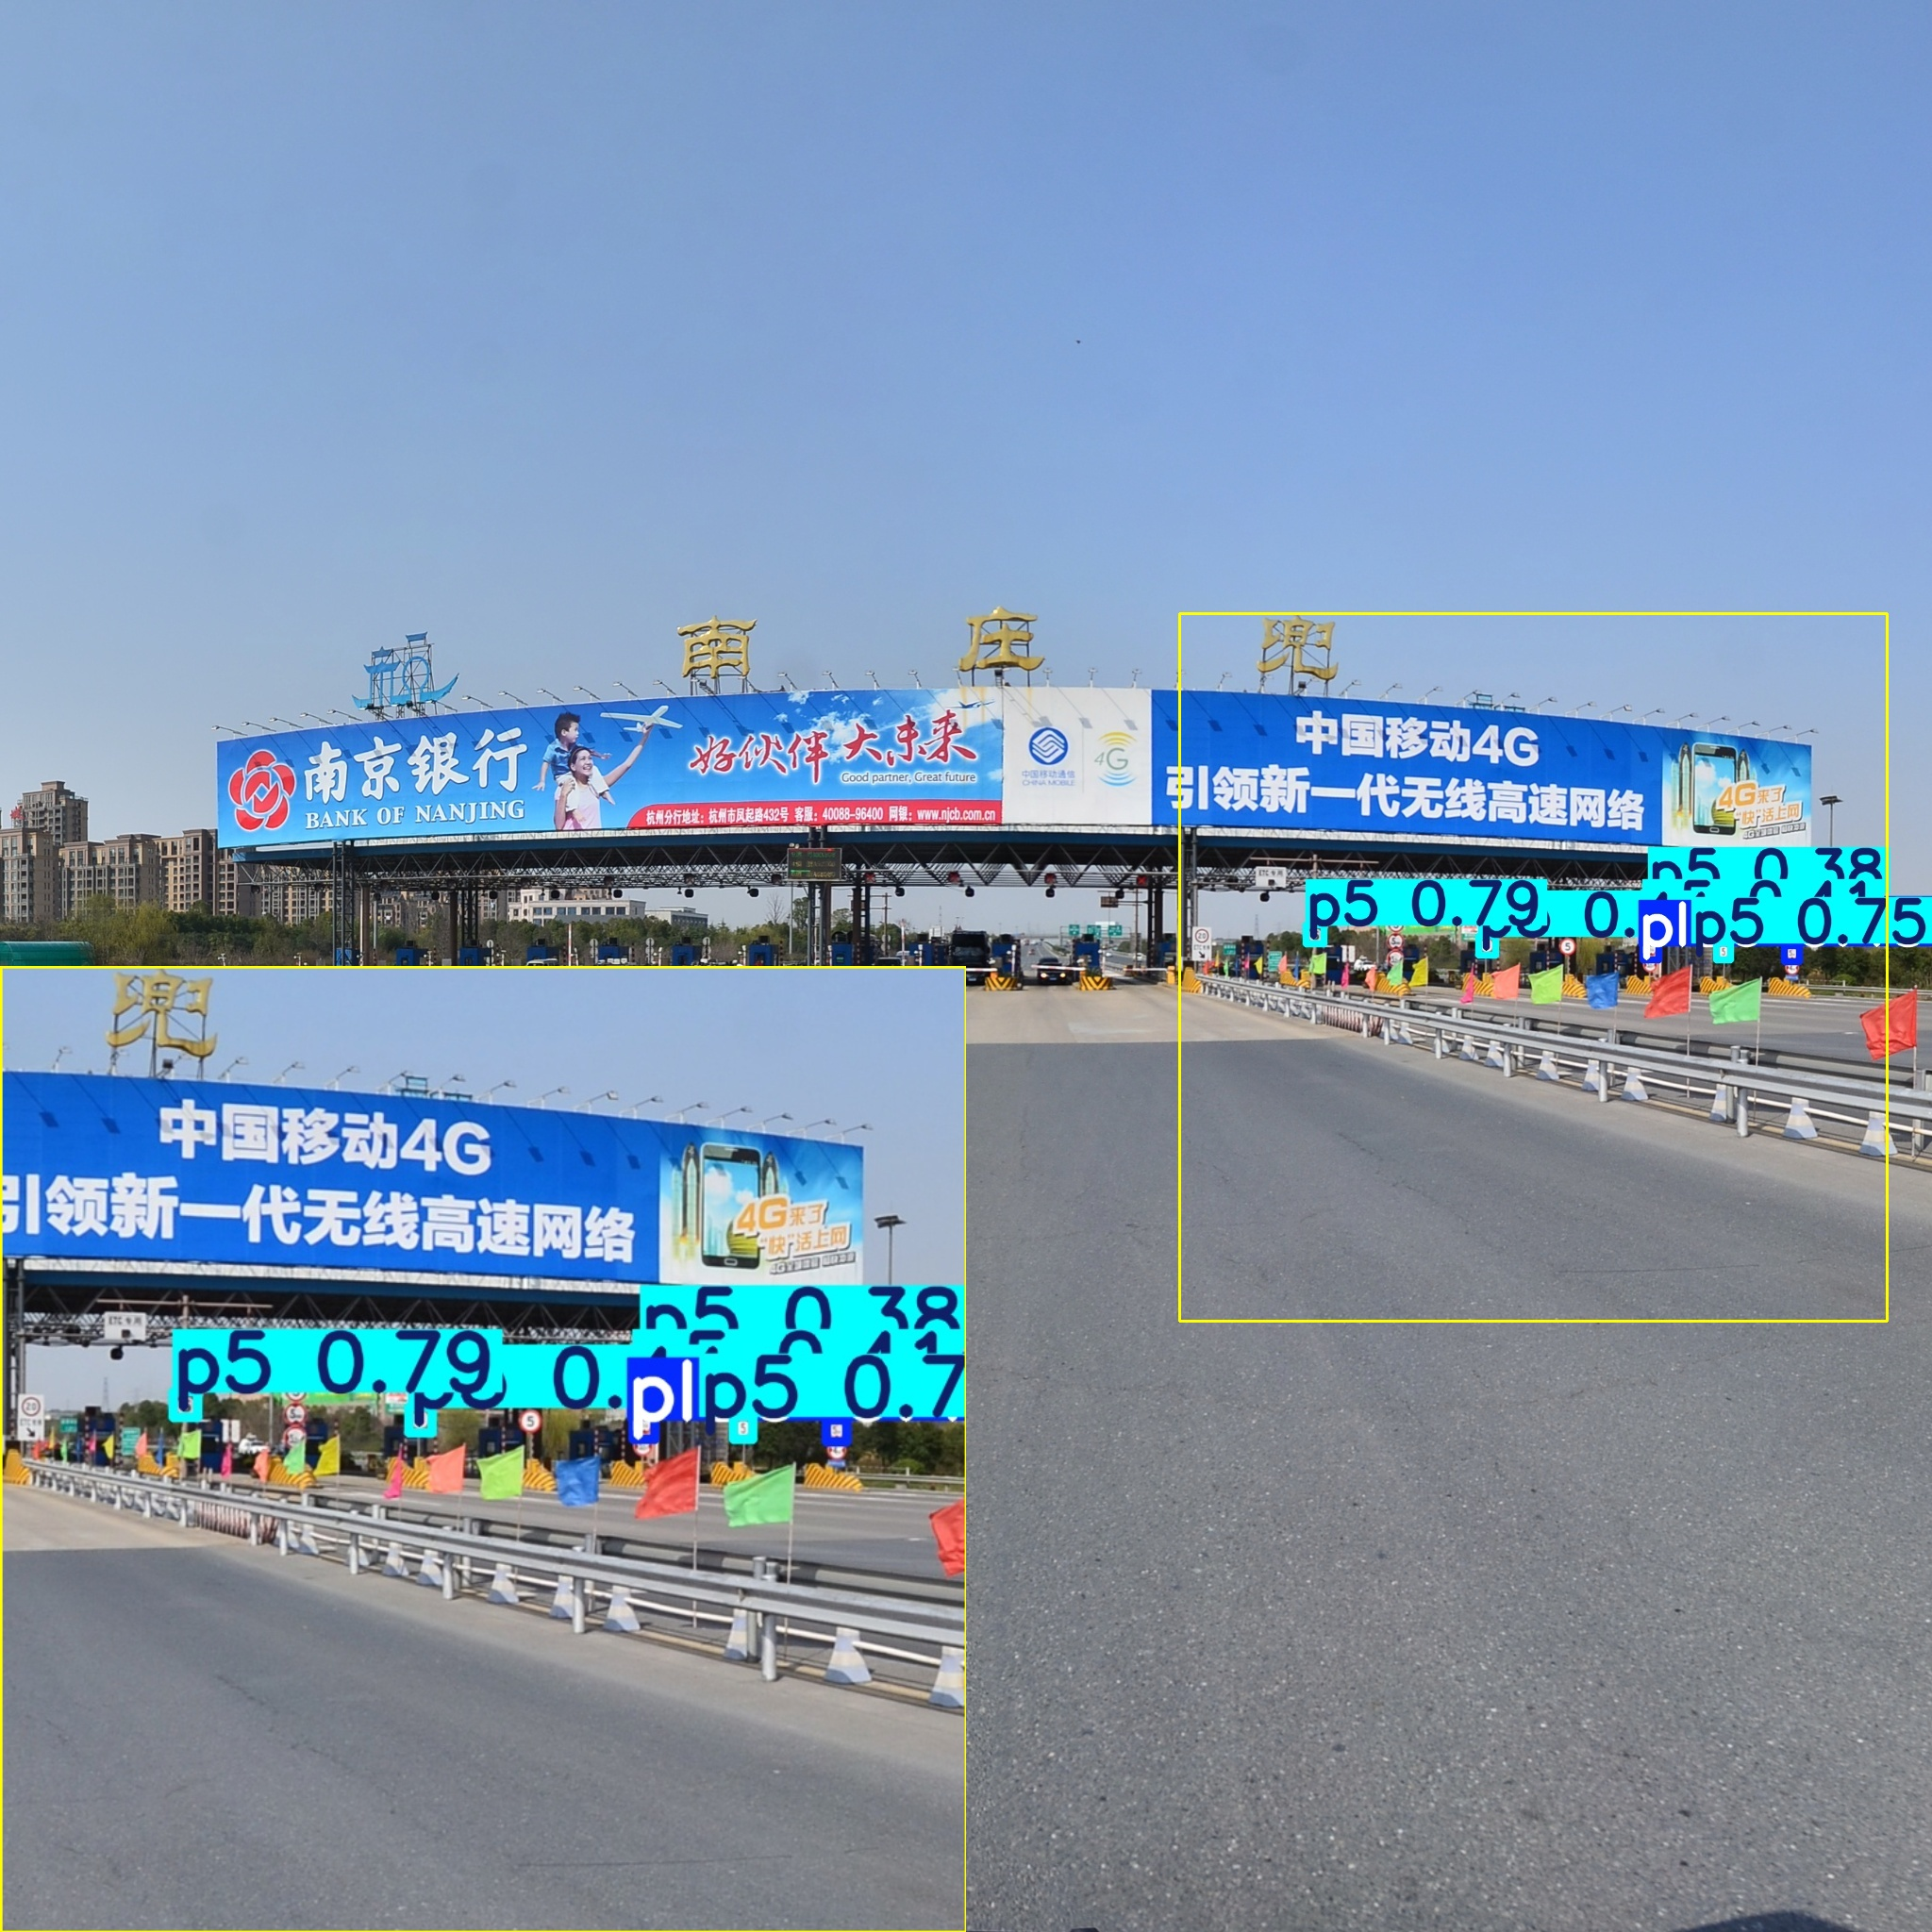
\includegraphics[width=0.33\textwidth]{../figure/v10s_tt100k_44171.jpg}%
        }
        \subfloat[YOLOv9s\label{fig:tt100k_2_9}]{%
            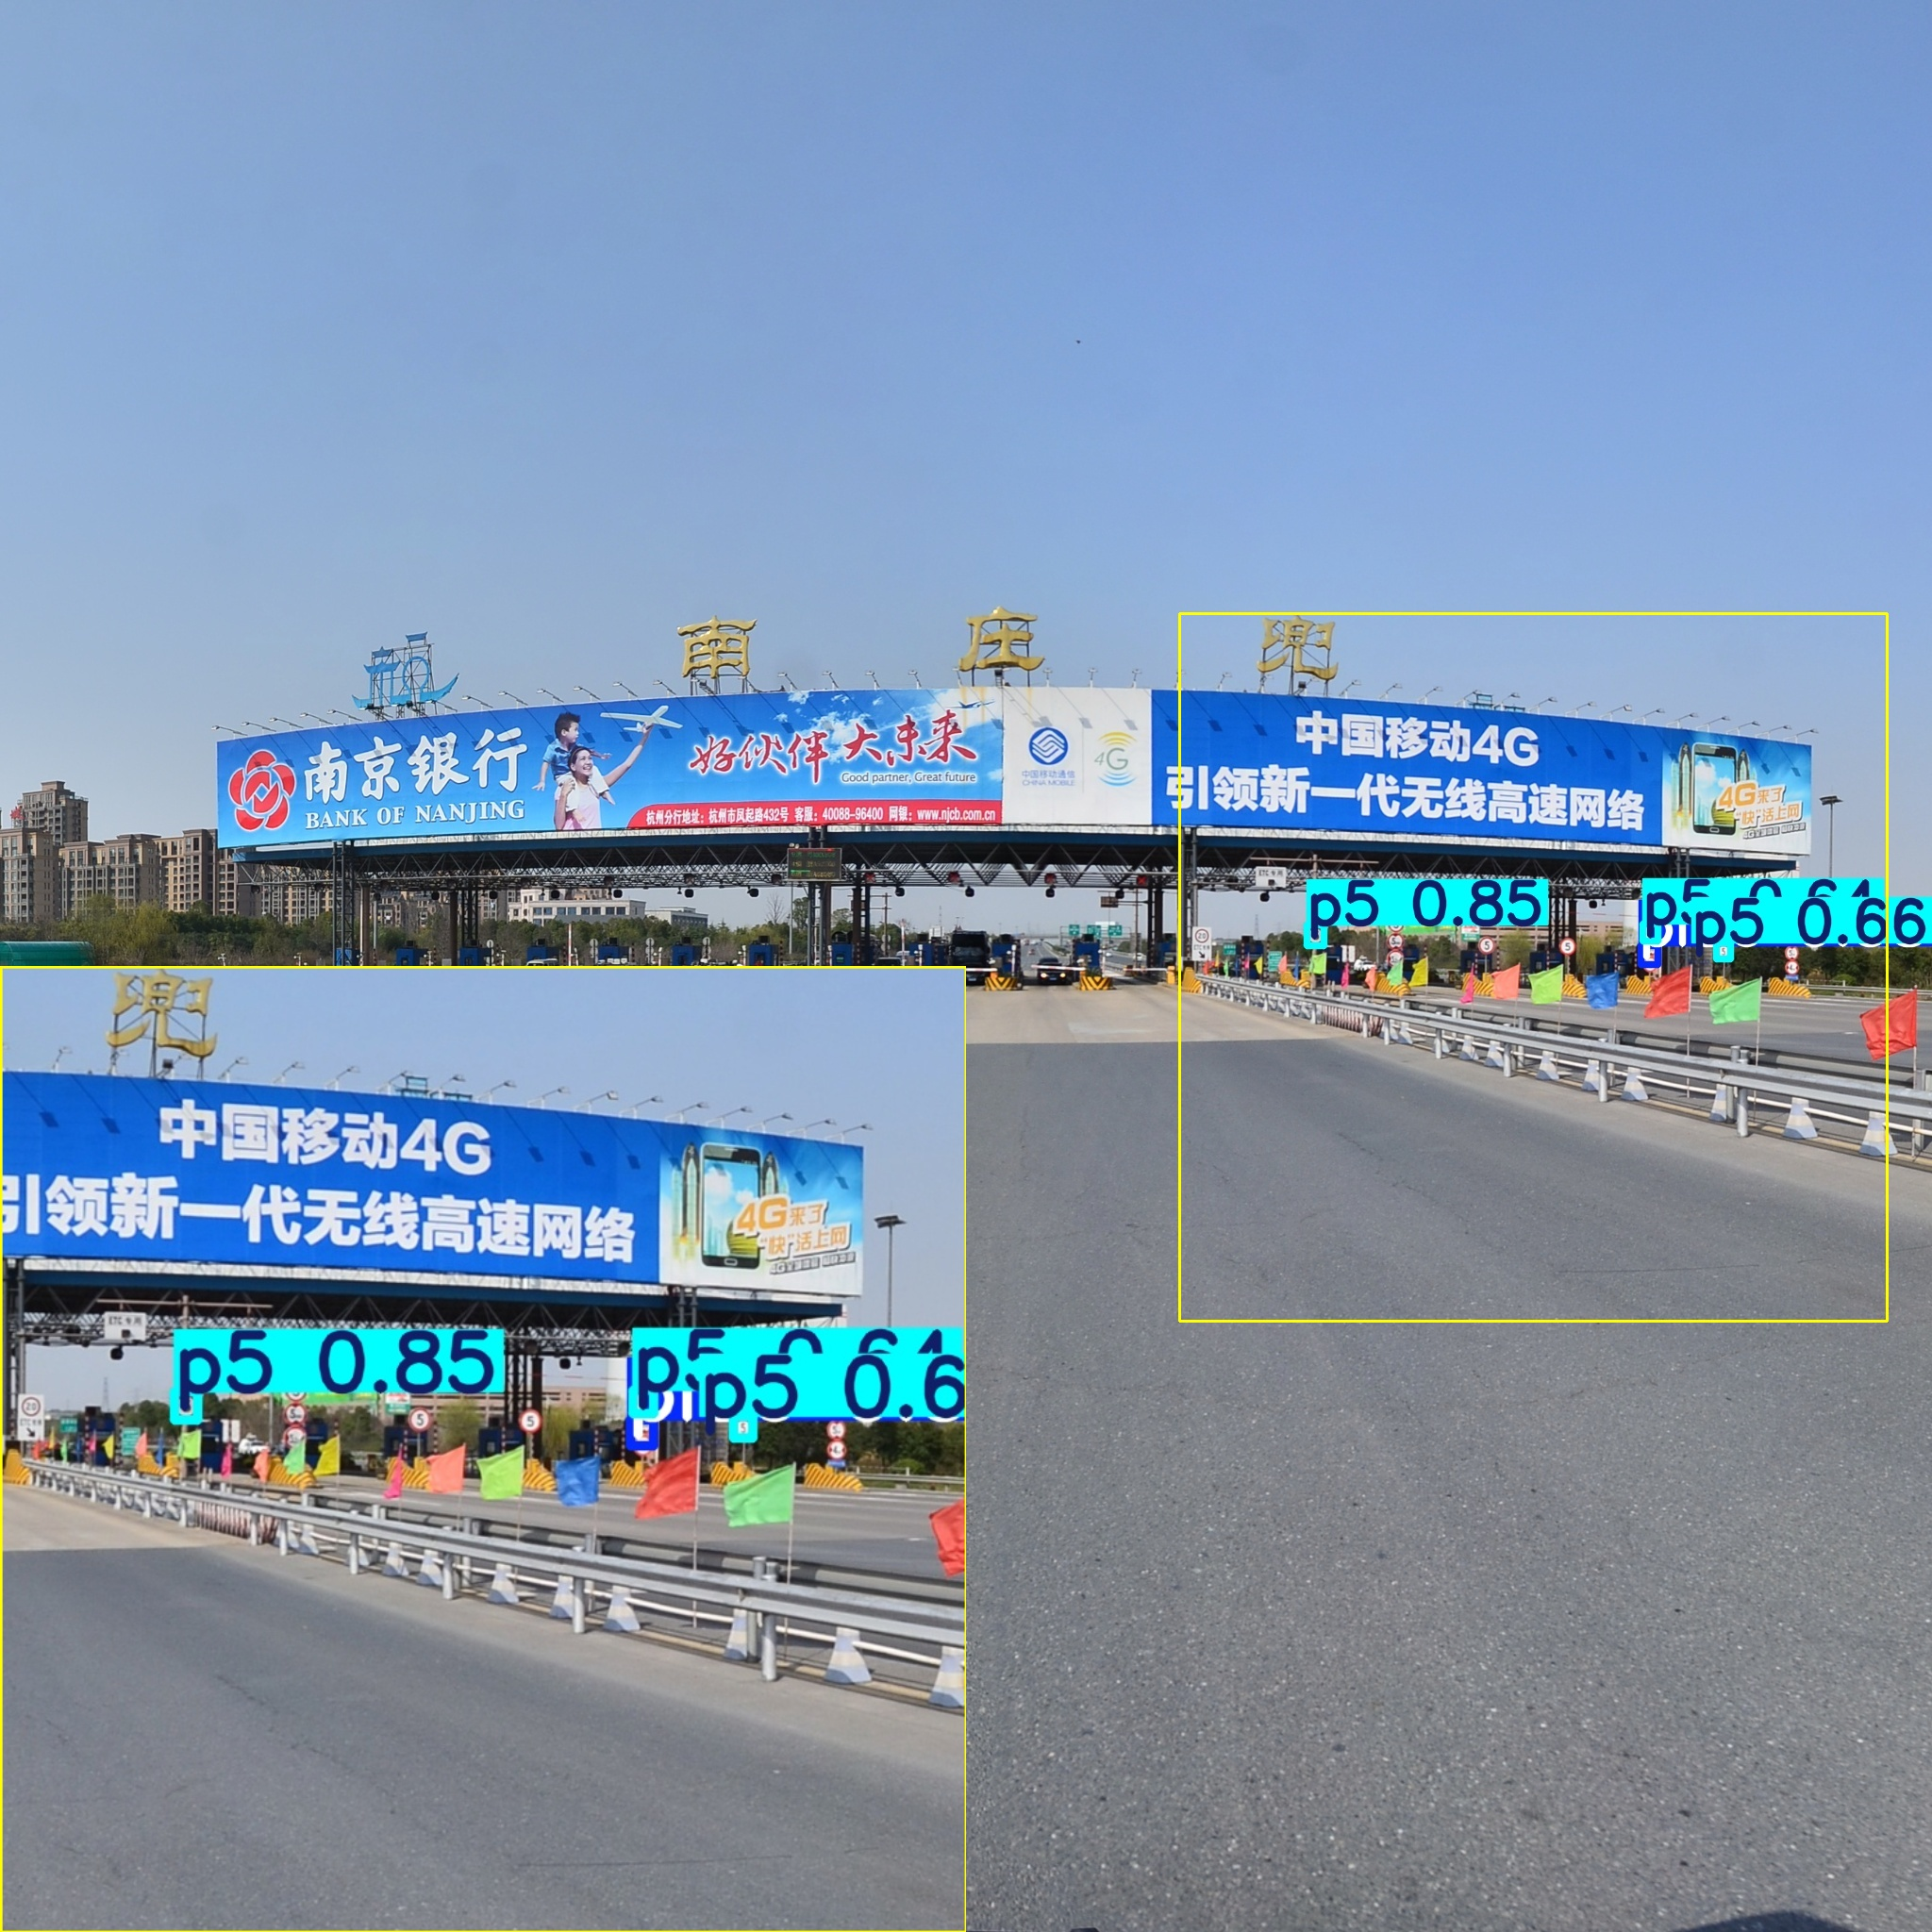
\includegraphics[width=0.33\textwidth]{../figure/v9s_tt100k_44171.jpg}%
        }
    \captionsetup{font=footnotesize}
    \bicaption{不同网络模型在TT100K数据集上的推理结果}{Some descriptions of the pictures in question.}
    \label{fig:tt100k_compare_2}
\end{figure}

在图\ref{fig:tt100k_compare_1}和图\ref{fig:tt100k_compare_2}的比较实验中,选择了TT100K数据集中具有复杂场景和干扰的图像。
图\ref{fig:tt100k_compare_1}显示,由于目标场景的复杂性,YOLOv9s无法检测到图片中的所有目标信息,YOLOv10s只能检测到一小部分目标信息,而YOLOv11s和EX-YOLO检测到更完整的目标信息。 可以看出,YOLOv9和YOLOv10在检测小目标方面仍然存在一些问题。 相比之下,EX-YOLO可以用低计算能力准确检测正确的目标。
图\ref{fig:tt100k_compare_2}显示,由于目标场景的复杂性,YOLOv9s无法检测到图片中的所有目标信息,YOLOv10s只能检测到一小部分目标信息,而YOLOv11s和EX-YOLO检测到更完整的目标信息。 可以看出,YOLOv9和YOLOv10在检测小目标方面仍然存在一些问题。 相比之下,EX-YOLO可以用低计算能力准确检测正确的目标。

\begin{figure}[htbp]
    \centering
        \subfloat[EX-YOLO\label{fig:vd_1_ex}]{%
        \includegraphics[width=0.4\textwidth]{../figure/ex-YOLOs_VisDrone_0000151_00348_d_0000133.jpg}} 
        \subfloat[YOLOv11s\label{fig:vd_1_11}]{%
        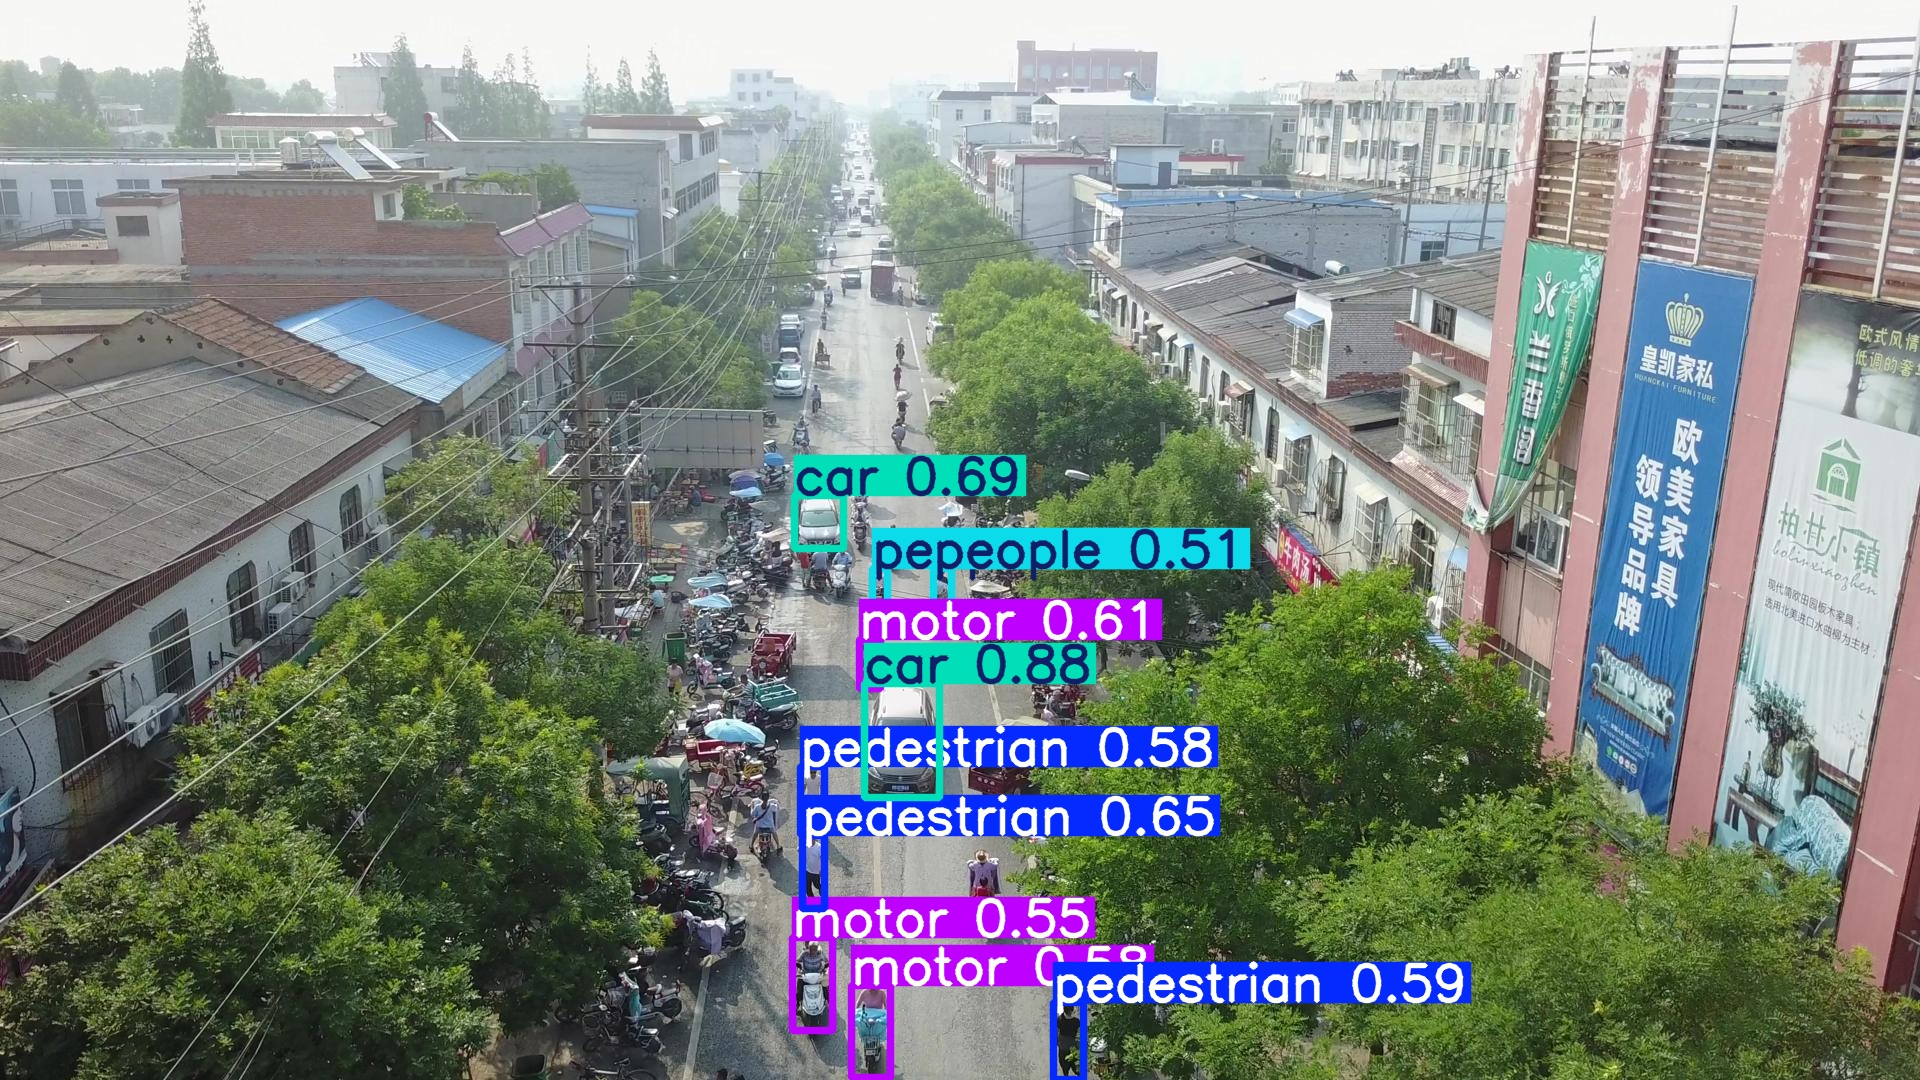
\includegraphics[width=0.4\textwidth]{../figure/v11s_VisDrone_0000151_00348_d_0000133.jpg}}
        \\
        \subfloat[YOLOv10s\label{fig:vd_1_10}]{%
        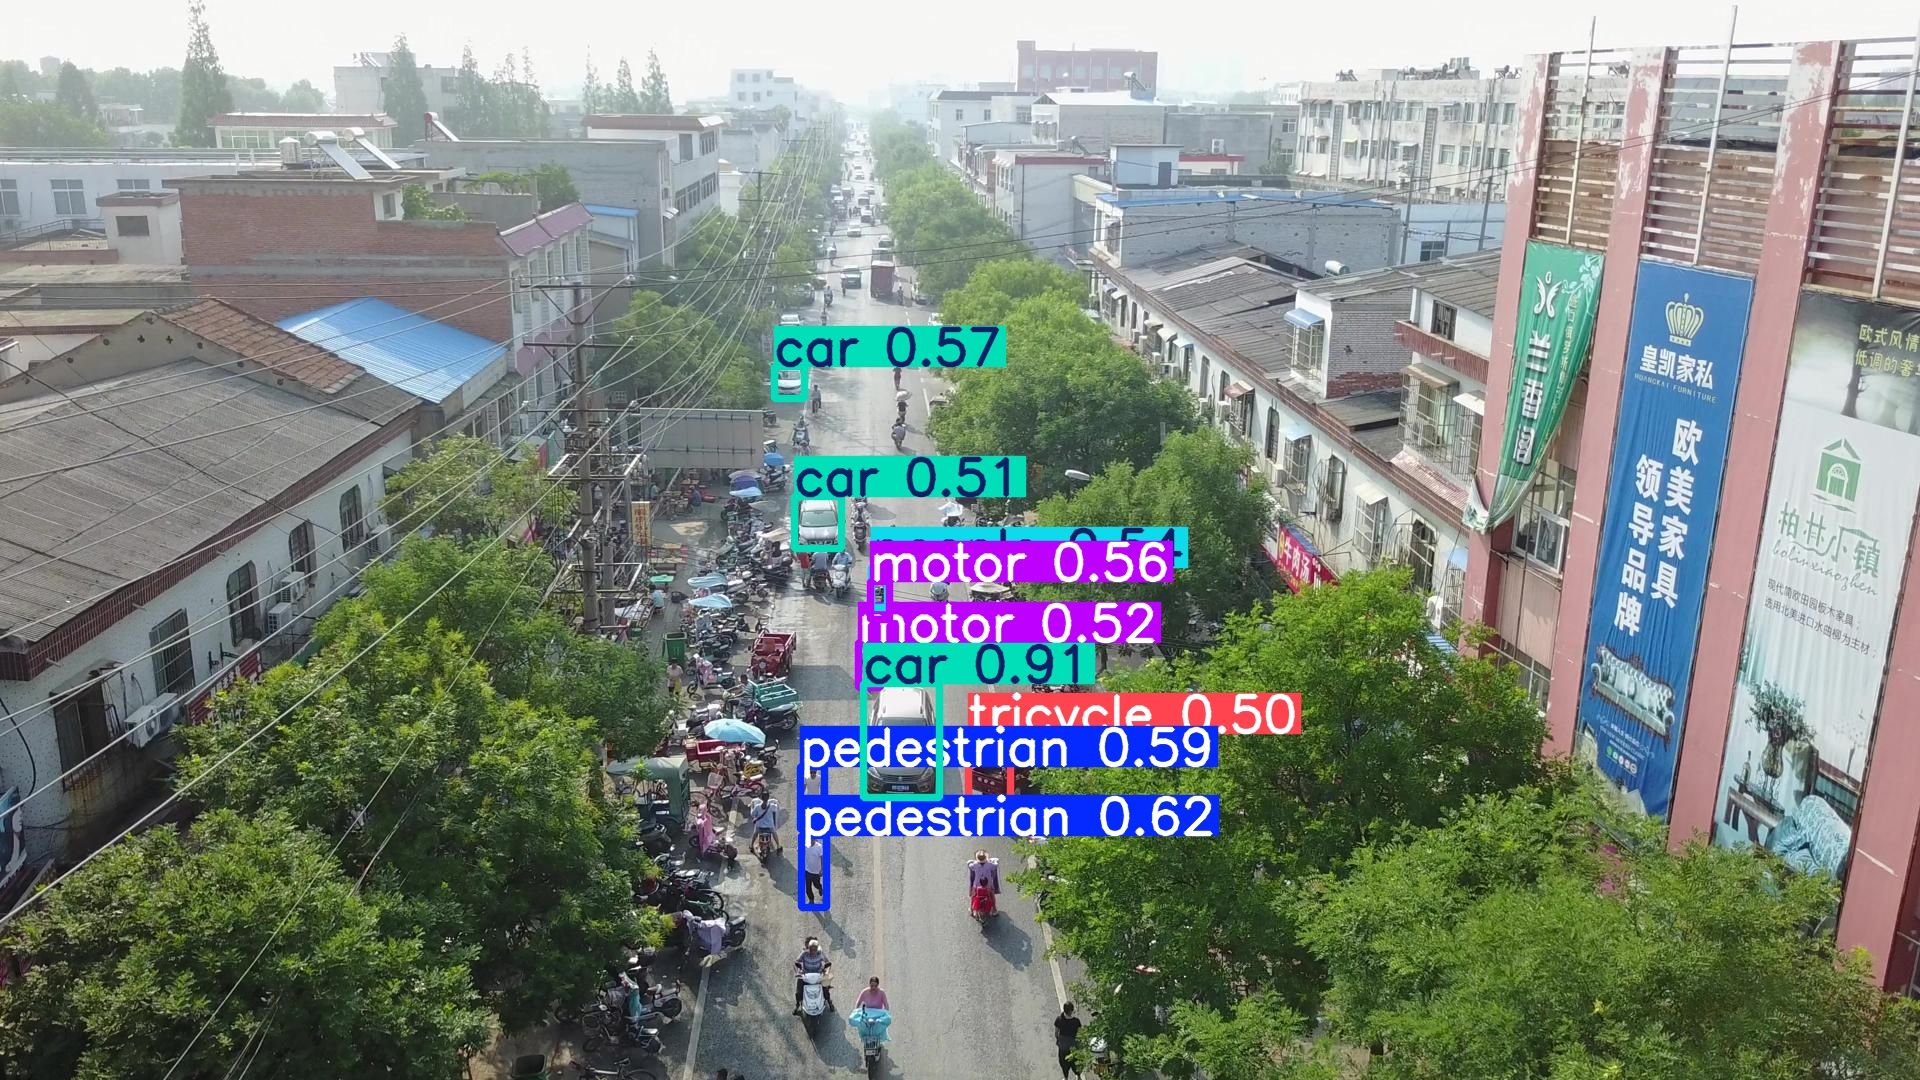
\includegraphics[width=0.4\textwidth]{../figure/v10s_VisDrone_0000151_00348_d_0000133.jpg}}
        \subfloat[YOLOv9s\label{fig:vd_1_9}]{%
        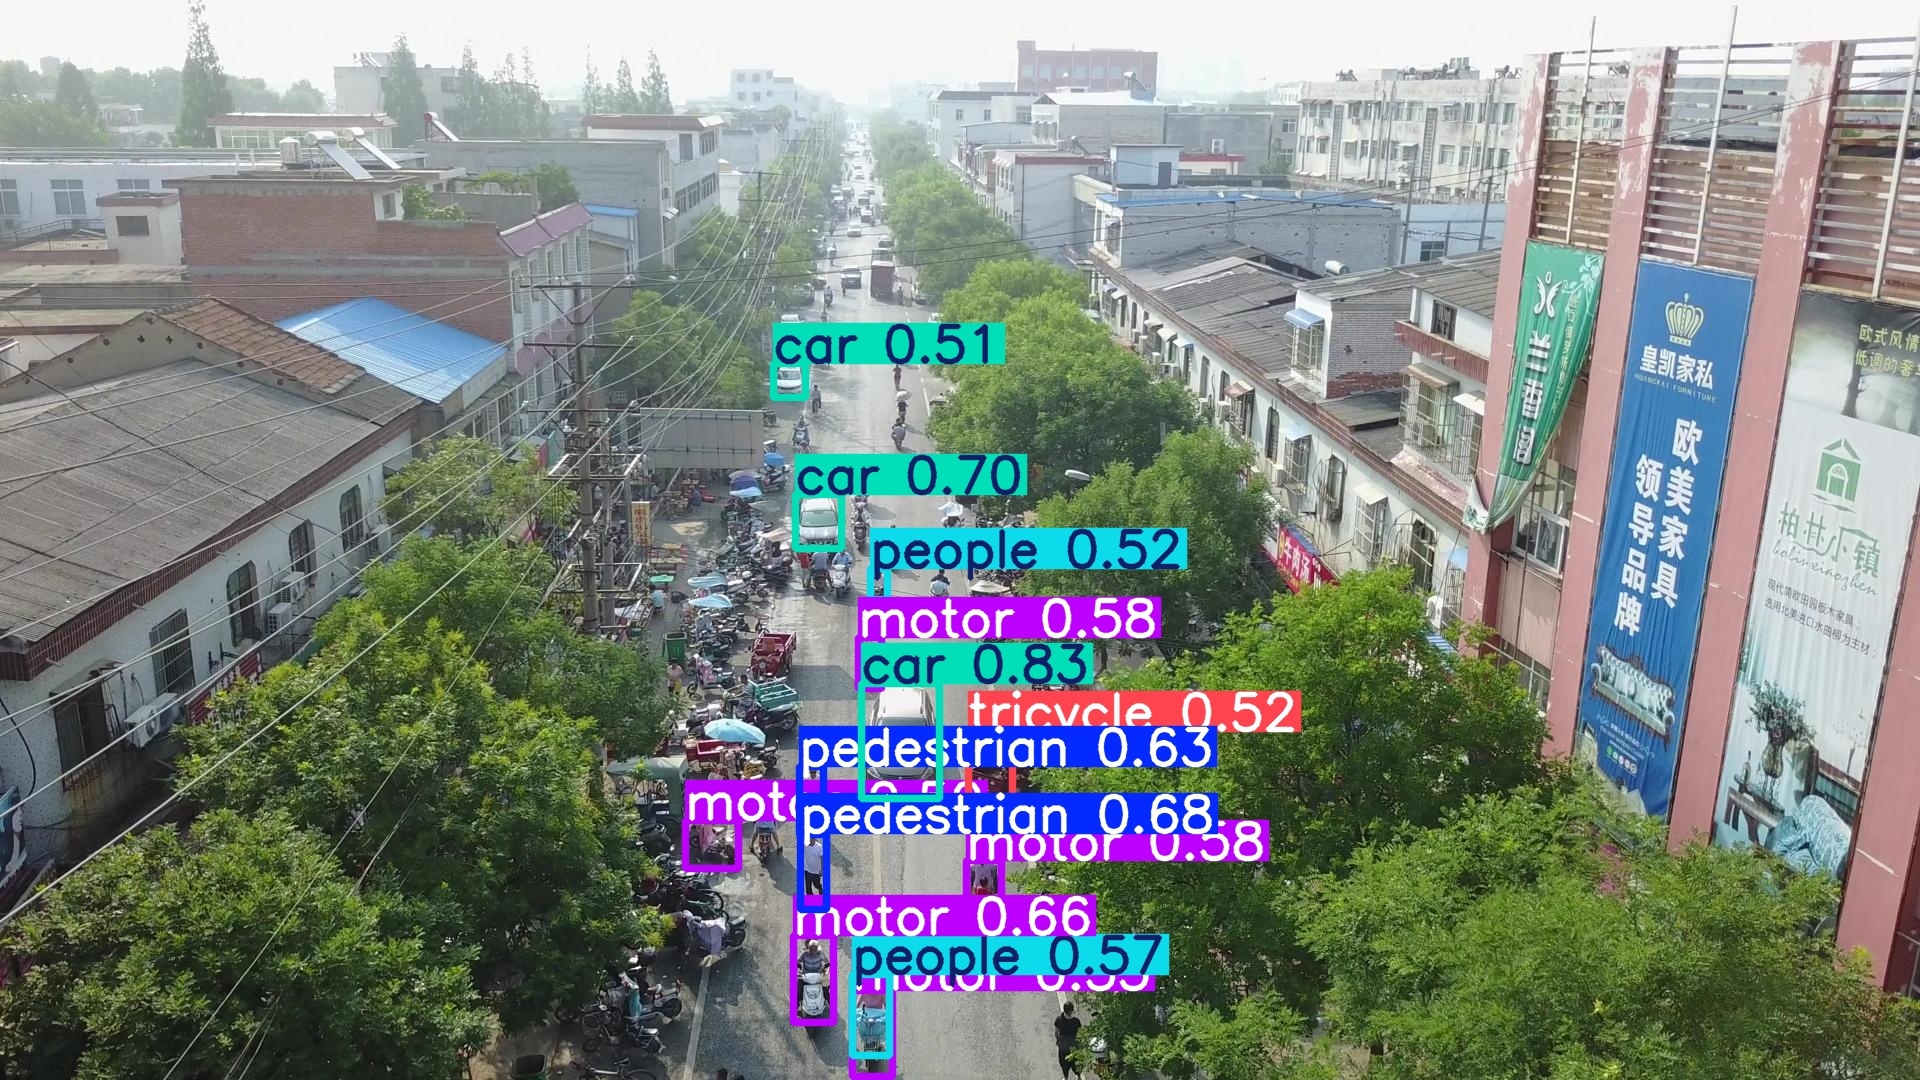
\includegraphics[width=0.4\textwidth]{../figure/v9s_VisDrone_0000151_00348_d_0000133.jpg}}
    \captionsetup{font=footnotesize}
    \bicaption{不同网络模型在VisDrone数据集上的推理结果}{Some descriptions of the pictures in question.}
    \label{fig:vd_compare_1}
\end{figure}

\begin{figure}[htbp]
    \centering
        \subfloat[EX-YOLO\label{fig:vd_2_ex}]{%
        \includegraphics[width=0.4\textwidth]{../figure/ex-YOLOs_VisDrone_0000151_00348_d_0000133.jpg}} 
        \subfloat[YOLOv11s\label{fig:vd_2_11}]{%
        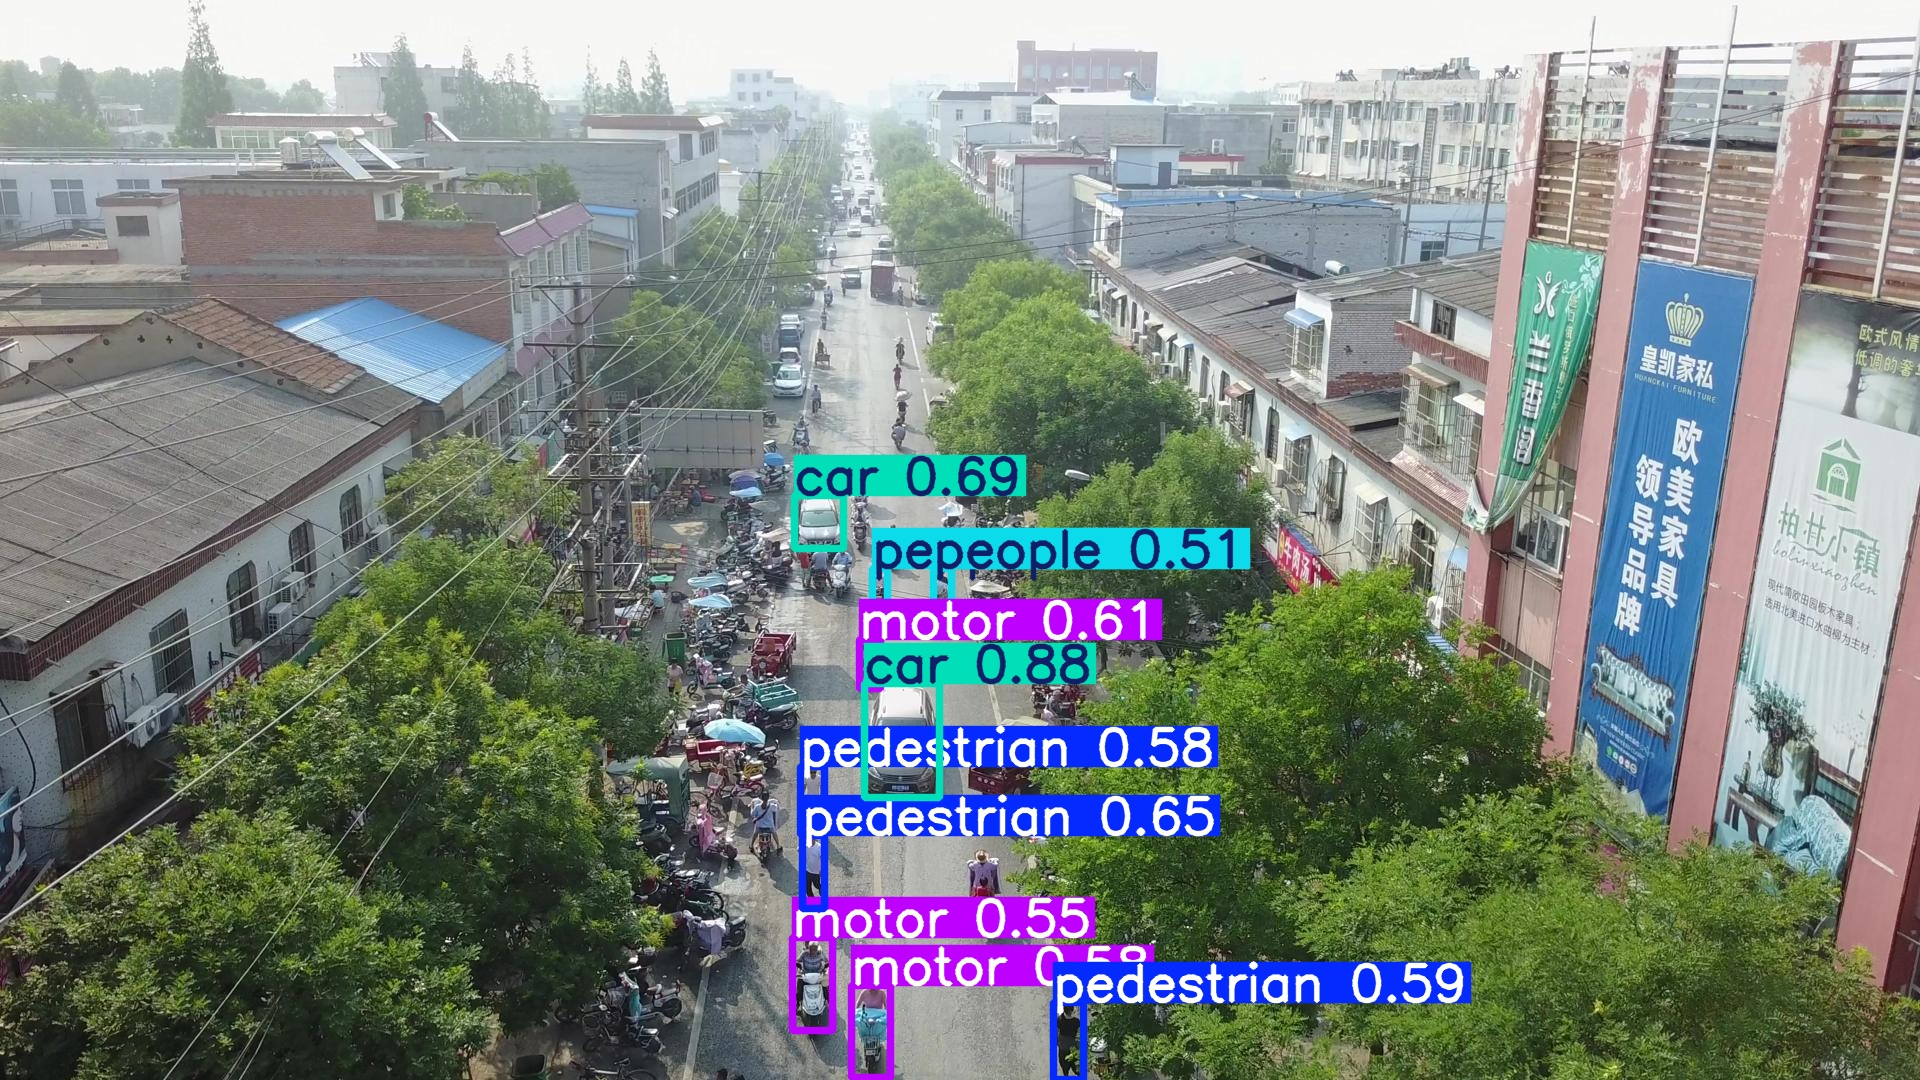
\includegraphics[width=0.4\textwidth]{../figure/v11s_VisDrone_0000151_00348_d_0000133.jpg}}
        \\
        \subfloat[YOLOv10s\label{fig:vd_2_10}]{%
        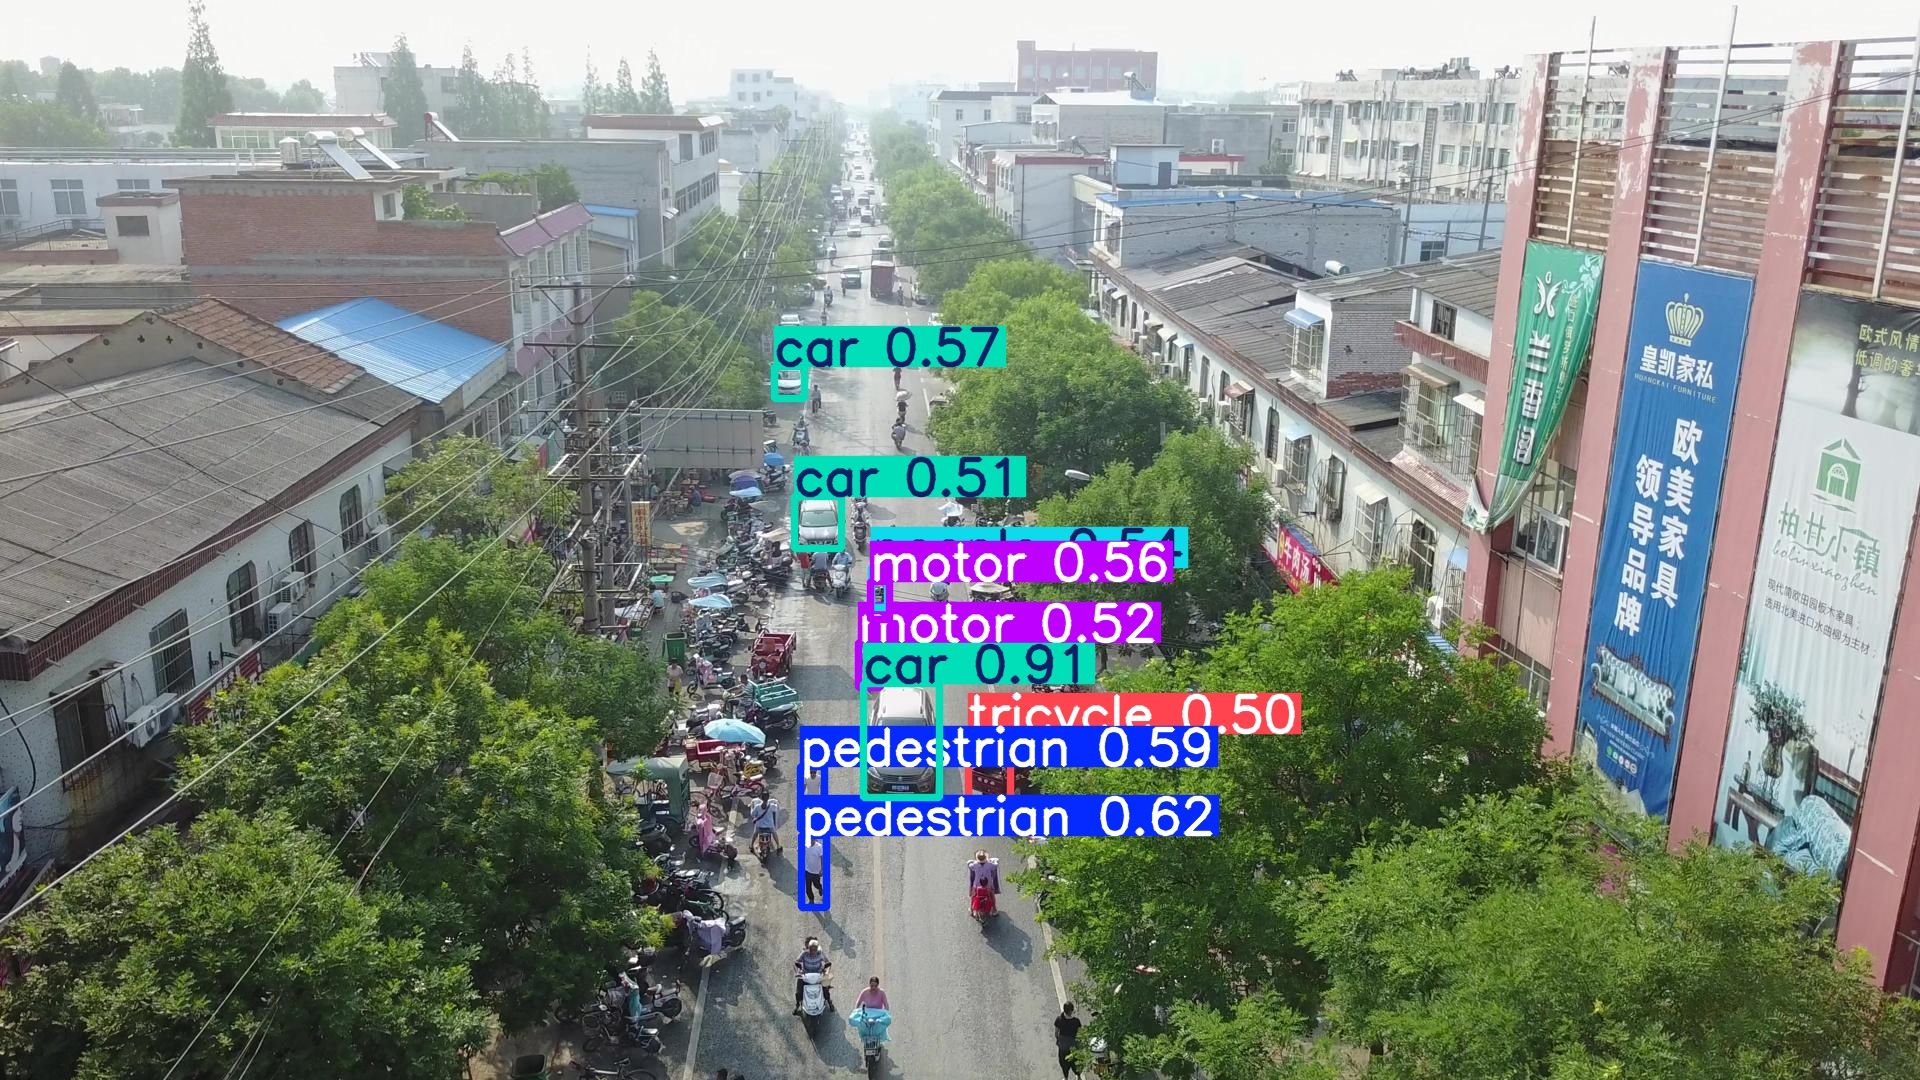
\includegraphics[width=0.4\textwidth]{../figure/v10s_VisDrone_0000151_00348_d_0000133.jpg}}
        \subfloat[YOLOv9s\label{fig:9}]{%
        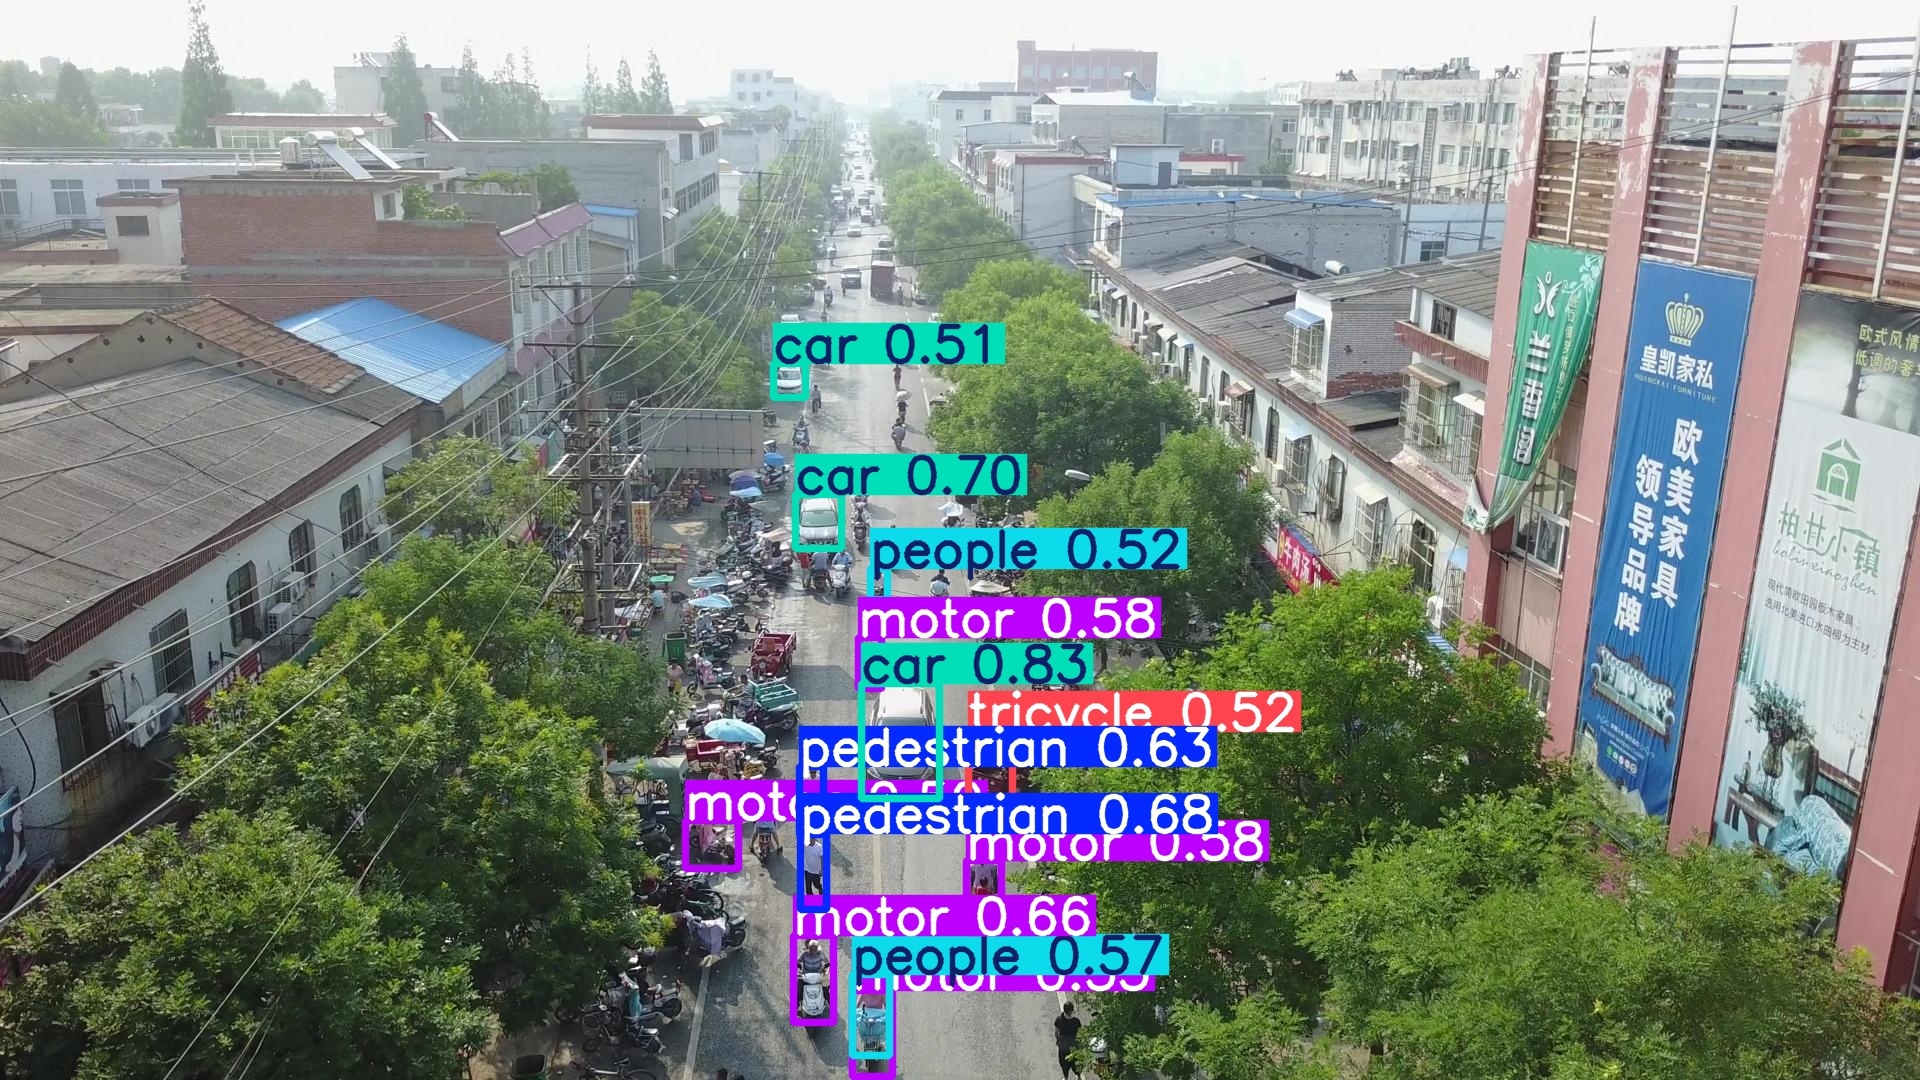
\includegraphics[width=0.4\textwidth]{../figure/v9s_VisDrone_0000151_00348_d_0000133.jpg}}
    \captionsetup{font=footnotesize}
    \bicaption{不同网络模型在VisDrone数据集上的推理结果}{Some descriptions of the pictures in question.}
    \label{fig:vd_compare_2}
\end{figure}

在图\ref{fig:vd_compare_1}和图\ref{fig:vd_compare_2}的比较实验中,在VisDrone数据集中选择具有复杂场景、小而密集的目标、各种目标、模糊和干扰的图像。
在图\ref{fig:vd_compare_1}中,所有模型的探测器都无法检测到所有检测目标,只能检测其中的一部分。 可以看出,YOLOv9s表现最好,这与其高mAP相吻合。 YOLOv10s和YOLOv11s在检测具有各种目标、模糊和干扰的小型密集目标方面仍然没有足够的性能。 相比之下,EX-YOLO可以在低计算量下准确检测更准确的目标,显示出接近YOLOv9s的检测性能,并且可以在复杂和重叠的场景中准确检测更多目标。 从图\ref{fig:vd_compare_1}可以看出,EX-YOLO的检测性能明显优于YOLOv10s和YOLOv11s,但略低于YOLOv9s。
在图\ref{fig:vd_compare_2}中,所有模型的探测器都无法检测到所有检测目标,只能检测其中的一部分。 可以看出,YOLOv9s表现最好,这与其高mAP相吻合。 YOLOv10s和YOLOv11s在检测具有各种目标、模糊和干扰的小型密集目标方面仍然没有足够的性能。 相比之下,EX-YOLO可以在低计算量下准确检测更准确的目标,显示出接近YOLOv9s的检测性能,并且可以在复杂和重叠的场景中准确检测更多目标。 从图\ref{fig:vd_compare_2}可以看出,EX-YOLO的检测性能明显优于YOLOv10s和YOLOv11s,但略低于YOLOv9s。

根据图\ref{fig:tt100k_compare_1}、图\ref{fig:tt100k_compare_2}、图\ref{fig:vd_compare_1}和图\ref{fig:vd_compare_2},当目标分布不均匀且分布不密集时,YOLOv11s可以实现更好的识别性能,而YOLOv9s可以在目标分布密集的条件下正确捕获更多目标。 EX-YOLO可以平衡这两种情况,以实现尽可能高的识别性能,这显然优于YOLOv10s,EX-YOLO大大减少了计算量。 这有利于无人机在面对复杂场景时识别小目标。

\subsection{本章小结}

本研究聚焦交通小目标检测难题,对 YOLOv11 网络进行深度改进,提出 EX-YOLO 算法。YOLOv11 以改进的 CSPDarknet 为骨干网络,其多层特征金字塔与 CSP 模块设计在特征提取的深度与广度上达成平衡,为复杂场景目标检测奠定基础。特征融合网络借助 FPN 和 PANet 实现多尺度特征融合与自适应加权,提升检测精度与鲁棒性。但传统 YOLO 框架在交通小目标检测中存在浅层特征图分辨率不足、跨尺度融合效率低及背景噪声干扰分类置信度等问题。

针对上述挑战,本研究提出创新改进措施。改进的特征融合模块 SPPC 融合 SPPF 的多尺度特征提取与 CAM 的特征增强能力,显著提升小目标特征捕获能力,提高 mAP。轻量化卷积模块 DBSS 结合深度可分离卷积(DSC)与 SimAM 注意力模块,在降低计算复杂度的同时保持高精度,减少模型参数量与计算量,适用于资源受限设备。引入的 NWD 损失函数与 DIoU 损失函数结合,精准计算预测框与真实框的空间和规模差异,增强小目标检测能力,尤其在小目标定位精度方面表现出色。

实验在 TT100K 和 VisDrone 数据集上验证 EX-YOLO 算法。结果显示,EX-YOLO 在参数量、计算量、精度、召回率和 FPS 等关键指标上综合性能优异。与 YOLOv11s、YOLOv10s 和 YOLOv9s 等基准模型相比,EX-YOLO 在保持较高检测精度的同时大幅降低计算量,平衡精度与效率。例如,在 TT100K 数据集上,EX-YOLO 的 mAP0.5 为 0.893,略低于 YOLOv9s 的 0.906,但计算量仅为其 62.5\%(17.0 GFLOPs 对比 27.2 GFLOPs)。在 VisDrone 数据集上,EX-YOLO 的 mAP0.5 与 YOLOv10s 相同(0.390),计算量却仅为后者的 62.8\%(15.4 GFLOPs 对比 24.5 GFLOPs)。消融实验进一步证实各改进模块的有效性,NWD 损失函数、SPPC 模块和 DBSS 模块在提升检测性能与优化计算效率方面发挥关键作用。

实验表明,EX-YOLO 算法在交通小目标检测领域竞争优势显著,尤其适用于资源受限场景。通过引入创新模块,本研究增强 YOLOv11 模型的小目标检测实用性,降低计算资源需求,使其更适配无人机等有限设备环境。未来,随着深度学习技术发展,EX-YOLO 算法有望在智能交通系统、无人机监控等领域发挥更大作用,助力高效精准的交通目标检测。